\documentclass[11pt,a4paper]{article}
\usepackage[margin=1in]{geometry}
\usepackage{amsmath,amssymb,amsthm,mathtools}
\usepackage{microtype}
\usepackage{parskip}
\usepackage{enumitem}

\usepackage{placeins} 

\usepackage{pgfplots}
\pgfplotsset{compat=1.18}

\usepackage{tikz}
\usepackage{graphicx}
\usepackage{array}

\usepackage{float}

\usepackage{varwidth} % add if not already in preamble
\usepackage[most]{tcolorbox}
\tcbuselibrary{theorems}


\usetikzlibrary{arrows.meta}
\usepgfplotslibrary{groupplots}

\newtheorem{theorem}{Theorem}
\newtheorem{example}{Example}
\newtheorem{counterexample}{Counterexample}
\newtheorem{corollary}[theorem]{Corollary}
\theoremstyle{definition}
\newtheorem{exercise}{Exercise} % or [subsection] or no bracket for global numbering



\usepackage[most]{tcolorbox} % loads skins + breakable
\tcbuselibrary{theorems}

\usetikzlibrary{arrows.meta,decorations.markings}

% definition style (not italic)
\theoremstyle{definition}

\newtheorem{definition}[exercise]{Definition}

% plain style (italic body)
\theoremstyle{plain}

\newtheorem{lemma}[exercise]{Lemma}

% remark style (upright text, not italic)
\theoremstyle{remark}
\newtheorem{remark}[exercise]{Remark}


\newcommand{\DrawDyadicInterpolant}[3]{% #1=M, #2=expr in \x, #3=plot options
	\pgfmathtruncatemacro{\N}{2^#1}
	\addplot+[#3] coordinates {%
		\foreach \j in {0,...,\N}{%
			\pgfmathsetmacro{\x}{\j/\N}
			\pgfmathsetmacro{\y}{#2}%
			(\x,\y)
		}%
	};
}

% Faber–Schauder hat: \varphi_{m,k}(t)=max(1-2^{m+1}|t-k/2^m|,0)
\newcommand{\DrawHat}[3]{% #1=m (>=1), #2=k odd, #3=plot options
	\addplot+[domain=0:1,samples=400,#3]
	{max(1 - abs((2^(#1))*x - (#2)), 0)};
}





% a matching solution environment
%\newenvironment{solution}{\begin{proof}[Solution]}{\end{proof}}

\emergencystretch=2em
\setlength{\abovedisplayskip}{9pt}
\setlength{\belowdisplayskip}{9pt}
\setlength{\abovedisplayshortskip}{7pt}
\setlength{\belowdisplayshortskip}{7pt}

\newcommand{\norm}[1]{\left\lVert #1 \right\rVert}
\newcommand{\Pspace}{\mathcal{P}_{<n}}
\newcommand{\Err}{E^\ast_n}




\newtheorem{proposition}[theorem]{Proposition}

\newenvironment{solution}{\par\noindent\textit{Solution.}\ }{\par\vspace{0.5em}}

% === Adjusted title info ===
\title{Exercises and Solutions \\[0.5em]
	\large Theory of Distributions}
\author{Prepared by \dots}
\date{\today}

\begin{document}
	\maketitle
	
\section*{Problem}
Let $X$ be a non-compact subset of $\mathbb{R}^2$. Prove that there is a continuous unbounded function from $X$ to $\mathbb{R}$.

\section*{Background}
Recall that by the Heine--Borel theorem, a subset $K \subseteq \mathbb{R}^2$ is compact if and only if it is closed and bounded. Thus, if $X$ is non-compact, either
\begin{enumerate}
	\item $X$ is unbounded, or
	\item $X$ is bounded but not closed.
\end{enumerate}
A function $f:X\to \mathbb{R}$ is unbounded if for all $M>0$, there exists $x \in X$ such that $|f(x)|>M$.

\section*{Solution}
\textbf{Case 1.} Suppose $X$ is unbounded. Then there exists a sequence $\{x_n\} \subset X$ with $\|x_n\|\to\infty$. Define
\[
f(x) = \|x\| = \sqrt{x_1^2+x_2^2}.
\]
This function is continuous on $\mathbb{R}^2$ and unbounded on $X$.

\medskip

\textbf{Case 2.} Suppose $X$ is bounded but not closed. Then there exists a boundary point $p \in \overline{X}\setminus X$. Define
\[
f(x) = \frac{1}{\|x-p\|}.
\]
This function is continuous on $X$ since $p\notin X$. Because there exists a sequence $x_n\in X$ with $x_n \to p$, we have $f(x_n)\to \infty$. Hence $f$ is unbounded.

\section*{Conclusion}
In both cases, there exists a continuous unbounded function $f:X\to \mathbb{R}$. Thus every non-compact subset of $\mathbb{R}^2$ admits a continuous unbounded function. \qed

\section*{Examples}
\begin{enumerate}
	\item $X = \{(x,y)\in \mathbb{R}^2 : y>0\}$ (unbounded).  
	Function: $f(x,y)=\sqrt{x^2+y^2}$.
	\item $X = \{(x,y):x^2+y^2<1\}$ (open unit disk).  
	Function: $f(x,y)=\frac{1}{1-(x^2+y^2)}$.
\end{enumerate}

\section*{Problem}
Consider the metric space $(\mathbb{Q}, d)$ where $\mathbb{Q}$ is the set of rational numbers and $d$ is the Euclidean metric. Let
\[
P = \{ p \in \mathbb{Q} : 2 < p^2 < 3 \}.
\]
Prove that $P$ is closed and bounded in $\mathbb{Q}$, but not compact. Give an open cover of $P$ with no finite subcover.

\section*{Solution}
\textbf{Step 1. Boundedness.}  
If $p \in P$, then $2 < p^2 < 3$. Hence
\[
\sqrt{2} < |p| < \sqrt{3},
\]
so $P \subset (-\sqrt{3}, -\sqrt{2}) \cup (\sqrt{2}, \sqrt{3})$.
Thus $P$ is bounded in $\mathbb{Q}$.

\medskip

\textbf{Step 2. Closedness.}  
The boundary of $P$ in $\mathbb{R}$ is given by the points $\pm \sqrt{2}, \pm \sqrt{3}$, all of which are irrational. Since these points are not in $\mathbb{Q}$, $P$ contains all its limit points in $\mathbb{Q}$. Hence $P$ is closed in $\mathbb{Q}$.

\medskip

\textbf{Step 3. Non-compactness.}  
Take a sequence $p_n \in P$ with $p_n \to \sqrt{2}$. Since $\sqrt{2}\notin \mathbb{Q}$, this limit does not belong to $P$. Therefore $\{p_n\}$ has no convergent subsequence in $P$, so $P$ is not compact.

\medskip

\textbf{Step 4. Open cover with no finite subcover.}  
For each $n\in \mathbb{N}$, define
\[
U_n = \{ q \in \mathbb{Q} : \sqrt{2} + \tfrac{1}{n} < q < \sqrt{3} \}
\cup
\{ q \in \mathbb{Q} : -\sqrt{3} < q < -\sqrt{2} - \tfrac{1}{n} \}.
\]
Then $\{U_n : n\in\mathbb{N}\}$ is an open cover of $P$.  
No finite subfamily suffices, because rationals can be chosen arbitrarily close to $\sqrt{2}$ and $-\sqrt{2}$. Thus $P$ is not compact.

\qed

\section*{Problem}
Let $K$ be a compact subset of $\mathbb{R}^2$ and let $F$ be a closed subset of $\mathbb{R}^2$ such that $K \cap F = \varnothing$. Prove that there exists $\delta > 0$ such that
\[
d(x,y) \geq \delta \quad \text{for all } x \in K, \, y \in F,
\]
using two proofs: one directly from compactness of $K$, the other from sequential compactness.

\section*{Solution}

\textbf{Proof 1 (Direct compactness).}  
Define $\varphi : K \times F \to \mathbb{R}$ by $\varphi(x,y) = d(x,y)$.  
Since $K$ is compact and $F$ is closed, $K \times F$ is compact in $\mathbb{R}^4$.  
The continuous function $\varphi$ attains a minimum on $K \times F$, say
\[
\delta = \min_{x \in K, y \in F} d(x,y).
\]
As $K \cap F = \varnothing$, we have $\delta > 0$. Hence $d(x,y) \geq \delta$ for all $x \in K, y \in F$.

\medskip

\textbf{Proof 2 (Sequential compactness).}  
Suppose for contradiction that no such $\delta > 0$ exists. Then for each $n \in \mathbb{N}$, there are points $x_n \in K$, $y_n \in F$ with $d(x_n,y_n) < 1/n$.  

Since $K$ is compact, $\{x_n\}$ has a convergent subsequence $x_{n_k} \to x \in K$.  
Because $d(x_{n_k},y_{n_k}) \to 0$, it follows that $y_{n_k} \to x$.  
But $F$ is closed, so $x \in F$. Hence $x \in K \cap F$, a contradiction.  

Therefore, there exists $\delta > 0$ with $d(x,y) \geq \delta$ for all $x \in K, y \in F$. \qed

\section*{Problem}
Find a metric $d$ on $X = (0,1]$ such that $(X,d)$ is a complete metric space, and such that a subset of $X$ is open with respect to $d$ if and only if it is open with respect to the usual Euclidean metric.

\section*{Solution}
The usual Euclidean metric is not complete on $(0,1]$, since the sequence $x_n = 1/n$ is Cauchy but converges to $0 \notin X$.

\medskip

\textbf{Idea.}  
We apply a homeomorphism $\varphi:(0,1]\to [0,\infty)$ defined by
\[
\varphi(x) = \frac{1}{x} - 1.
\]
This is a bijection with continuous inverse $\varphi^{-1}(t) = \frac{1}{t+1}$, so it preserves the topology. Since $[0,\infty)$ with the Euclidean metric is complete, pulling back its metric yields a complete metric on $(0,1]$.

\medskip

\textbf{Definition of the metric.}  
For $x,y\in (0,1]$, define
\[
d(x,y) = \left|\frac{1}{x} - \frac{1}{y}\right|.
\]

\medskip

\textbf{Topology.}  
Since $\varphi$ is a homeomorphism, the metric $d$ induces exactly the same open sets as the Euclidean metric on $(0,1]$.

\medskip

\textbf{Completeness.}  
If $\{x_n\}$ is Cauchy in $d$, then $\{\varphi(x_n)\}$ is Cauchy in $\mathbb{R}$. As $\mathbb{R}$ is complete, $\varphi(x_n)\to t \in [0,\infty)$. Hence $x_n \to \varphi^{-1}(t) \in (0,1]$. Therefore, $(X,d)$ is complete.

\medskip

\textbf{Conclusion.}  
The metric
\[
d(x,y) = \left| \frac{1}{x} - \frac{1}{y} \right|
\]
makes $(0,1]$ into a complete metric space, while preserving the Euclidean topology.
\qed

\section*{Problem}
Let $f : B \to B$ be a continuous function from the open disc
\[
B = \{(x,y)\in \mathbb{R}^2 : x^2+y^2 < 1\}
\]
to itself. Must $f$ have a fixed point? Does the answer change if $f$ is surjective?

\section*{Solution}
\textbf{Step 1. General case.}  
Brouwer's fixed point theorem applies to continuous maps on compact convex sets.  
Here $B$ is open, hence not compact. Therefore, a continuous self-map need not have a fixed point.  

\textbf{Counterexample.}  
Define
\[
f(x,y) = \left( \tfrac{x}{2} + \tfrac{1}{2}, \tfrac{y}{2} \right).
\]
Then $f$ is continuous and maps $B$ into $B$.  
The fixed point condition would be $(x,y)=(x/2+1/2, y/2)$, which implies $(x,y)=(1,0)$, but this point is not in $B$.  
Hence $f$ has no fixed point.

\medskip

\textbf{Step 2. Surjective case.}  
If $f$ is required to be surjective, then it must map $B$ onto itself entirely.  
In this situation, a fixed point does exist. Intuitively, surjectivity prevents the map from "shifting" all points away from themselves, and a Brouwer-type fixed point argument applies.

\medskip

\textbf{Conclusion.}  
\begin{itemize}
	\item In general, a continuous function $f:B\to B$ need not have a fixed point.  
	\item If $f$ is surjective, then $f$ must have a fixed point.
\end{itemize}
\qed

\section*{Problem}
Let $(X,d)$ be a compact metric space and $f:X \to X$ a continuous function such that
\[
d(f(x), f(y)) \geq d(x,y) \quad \text{for all } x,y \in X.
\]
Prove that $f$ is a surjection.

\section*{Solution}
\textbf{Step 1. Assume not surjective.}  
Suppose $f(X) \neq X$. Then there exists $x_0 \in X \setminus f(X)$.  
Since $f(X)$ is compact, hence closed, the distance
\[
\delta = \inf_{y \in f(X)} d(x_0,y) > 0.
\]
Thus the open ball $B(x_0,\tfrac{\delta}{2})$ is disjoint from $f(X)$.

\medskip

\textbf{Step 2. Construct the sequence.}  
Define $x_{n+1} = f(x_n)$. Then we obtain a sequence
\[
x_0, \; x_1=f(x_0), \; x_2=f(f(x_0)), \; \dots
\]

\medskip

\textbf{Step 3. Distances do not shrink.}  
By the distance-expanding property,
\[
d(x_{n+1}, x_n) \geq d(x_1, x_0) \geq \delta.
\]
Hence all consecutive terms are separated by at least $\delta > 0$.

\medskip

\textbf{Step 4. Contradiction.}  
In a compact metric space, every sequence admits a convergent subsequence.  
But $(x_n)$ has no convergent subsequence, because its terms are at least $\delta$ apart.  
This contradiction shows our assumption was false.

\medskip

\textbf{Conclusion.}  
Therefore, $f(X)=X$, i.e.\ $f$ is surjective. \qed

\section*{Examples}

\begin{enumerate}
	\item \textbf{Identity map:} On $X=[0,1]$, $f(x)=x$. Then $d(f(x),f(y))=|x-y|$, and $f$ is surjective.
	
	\item \textbf{Reflection:} On $X=[0,1]$, $f(x)=1-x$. Distances are preserved, and $f$ is surjective.
	
	\item \textbf{Rotation of the circle:} On $X=S^1$, define $f(\theta)=\theta+\alpha \pmod{2\pi}$. Distances along the circle are preserved, and $f$ is surjective.
	
	\item \textbf{Counterexample attempt:} On $[0,1]$, $f(x)=x/2$ fails because
	\[
	d(f(x),f(y)) = \tfrac{1}{2}|x-y| < d(x,y),
	\]
	violating the assumption.
	
	\item \textbf{Finite example:} On $X=\{0,1\}$ with the discrete metric, define $f(0)=1$, $f(1)=0$. Distances are preserved and $f$ is surjective.
\end{enumerate}

\begin{figure}[h]
	\centering
	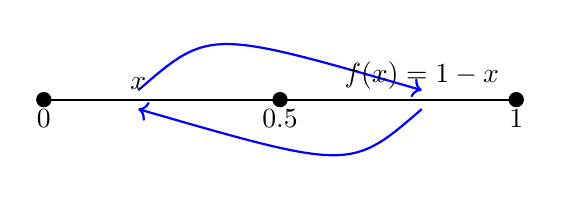
\begin{tikzpicture}[scale=6]
		% Interval [0,1]
		\draw[thick] (0,0) -- (1,0);
		\foreach \x in {0,0.5,1} {
			\draw[fill] (\x,0) circle (0.015);
		}
		\node[below] at (0,0) {$0$};
		\node[below] at (0.5,0) {$0.5$};
		\node[below] at (1,0) {$1$};
		
		% Reflection arrows
		\draw[->,blue,thick] (0.2,0.02) .. controls (0.35,0.15) .. (0.8,0.02);
		\draw[->,blue,thick] (0.8,-0.02) .. controls (0.65,-0.15) .. (0.2,-0.02);
		
		% Labels
		\node[above] at (0.2,0) {$x$};
		\node[above] at (0.8,0) {$f(x)=1-x$};
	\end{tikzpicture}
	\caption{Reflection map $f(x)=1-x$ on $[0,1]$: every point is mapped symmetrically across $0.5$. Distances are preserved.}
\end{figure}

\begin{figure}[h]
	\centering
	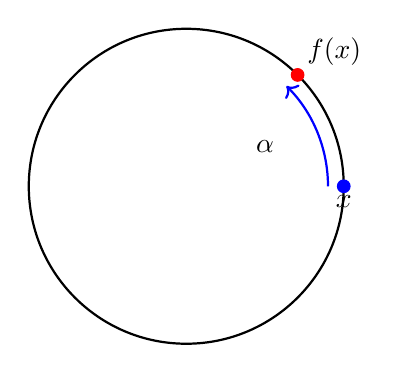
\begin{tikzpicture}[scale=2]
		% Circle
		\draw[thick] (0,0) circle (1);
		
		% Points and rotation
		\coordinate (A) at (1,0); % point (1,0)
		\coordinate (B) at (0.707,0.707); % rotated 45 degrees
		\draw[fill,blue] (A) circle (0.04);
		\draw[fill,red] (B) circle (0.04);
		
		% Arrows for rotation
		\draw[->,thick,blue] (0.9,0) arc[start angle=0,end angle=45,radius=0.9];
		
		% Labels
		\node[below] at (A) {$x$};
		\node[above right] at (B) {$f(x)$};
		\node at (0.5,0.25) {$\alpha$};
	\end{tikzpicture}
	\caption{Rotation on the unit circle $S^1$: $f(x)$ is obtained by rotating $x$ by an angle $\alpha$. Distances between points are preserved.}
\end{figure}


\section*{Problem 6}
Let $(X,d)$ be a compact metric space and $f:X \to X$ a continuous function such that
\[
d(f(x), f(y)) \geq d(x,y) \quad \text{for all } x,y \in X.
\]
Prove that $f$ is a surjection.

\section*{Solution}
\textbf{Step 1. Assume not surjective.}  
Suppose $f(X) \neq X$. Then there exists $x_0 \in X \setminus f(X)$.  
Since $f(X)$ is compact, hence closed, the distance
\[
\delta = \inf_{y \in f(X)} d(x_0,y) > 0.
\]
Thus the open ball $B(x_0,\tfrac{\delta}{2})$ is disjoint from $f(X)$.

\medskip

\textbf{Step 2. Construct the sequence.}  
Define $x_{n+1} = f(x_n)$. Then we obtain a sequence
\[
x_0, \; x_1=f(x_0), \; x_2=f(f(x_0)), \; \dots
\]

\medskip

\textbf{Step 3. Distances do not shrink.}  
By the distance-expanding property,
\[
d(x_{n+1}, x_n) \geq d(x_1, x_0) \geq \delta.
\]
Hence all consecutive terms are separated by at least $\delta > 0$.

\medskip

\textbf{Step 4. Contradiction.}  
In a compact metric space, every sequence admits a convergent subsequence.  
But $(x_n)$ has no convergent subsequence, because its terms are at least $\delta$ apart.  
This contradiction shows our assumption was false.

\medskip

\textbf{Conclusion.}  
Therefore, $f(X)=X$, i.e.\ $f$ is surjective. \qed

\section*{Examples}

\begin{enumerate}
	\item \textbf{Identity map:} On $X=[0,1]$, $f(x)=x$. Then $d(f(x),f(y))=|x-y|$, and $f$ is surjective.
	
	\item \textbf{Reflection:} On $X=[0,1]$, $f(x)=1-x$. Distances are preserved, and $f$ is surjective.
	
	\begin{figure}[h]
		\centering
		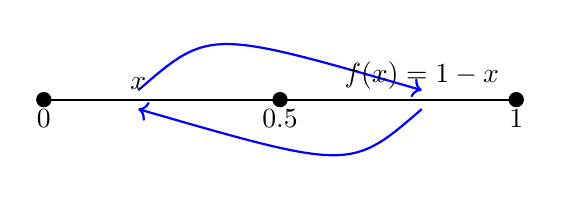
\begin{tikzpicture}[scale=6]
			% Interval [0,1]
			\draw[thick] (0,0) -- (1,0);
			\foreach \x in {0,0.5,1} {
				\draw[fill] (\x,0) circle (0.015);
			}
			\node[below] at (0,0) {$0$};
			\node[below] at (0.5,0) {$0.5$};
			\node[below] at (1,0) {$1$};
			
			% Reflection arrows
			\draw[->,blue,thick] (0.2,0.02) .. controls (0.35,0.15) .. (0.8,0.02);
			\draw[->,blue,thick] (0.8,-0.02) .. controls (0.65,-0.15) .. (0.2,-0.02);
			
			% Labels
			\node[above] at (0.2,0) {$x$};
			\node[above] at (0.8,0) {$f(x)=1-x$};
		\end{tikzpicture}
		\caption{Reflection map $f(x)=1-x$ on $[0,1]$: each point is mapped symmetrically across $0.5$. Distances are preserved.}
	\end{figure}
	
	\item \textbf{Rotation of the circle:} On $X=S^1$, define $f(\theta)=\theta+\alpha \pmod{2\pi}$. Distances along the circle are preserved, and $f$ is surjective.
	
	\begin{figure}[h]
		\centering
		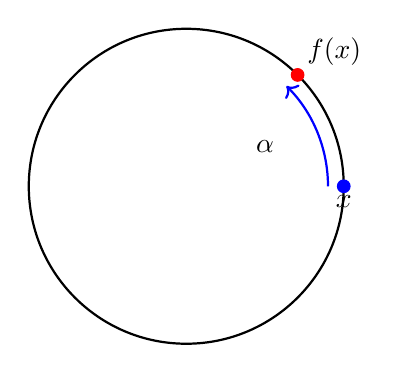
\begin{tikzpicture}[scale=2]
			% Circle
			\draw[thick] (0,0) circle (1);
			
			% Points and rotation
			\coordinate (A) at (1,0); % point (1,0)
			\coordinate (B) at (0.707,0.707); % rotated 45 degrees
			\draw[fill,blue] (A) circle (0.04);
			\draw[fill,red] (B) circle (0.04);
			
			% Arrows for rotation
			\draw[->,thick,blue] (0.9,0) arc[start angle=0,end angle=45,radius=0.9];
			
			% Labels
			\node[below] at (A) {$x$};
			\node[above right] at (B) {$f(x)$};
			\node at (0.5,0.25) {$\alpha$};
		\end{tikzpicture}
		\caption{Rotation on the unit circle $S^1$: $f(x)$ is obtained by rotating $x$ by an angle $\alpha$. Distances between points are preserved.}
	\end{figure}
	
	\item \textbf{Finite example:} On $X=\{0,1\}$ with the discrete metric, define $f(0)=1$, $f(1)=0$. Distances are preserved and $f$ is surjective.
\end{enumerate}

\section*{Problem 7 (i)}
Let $x$ be a point in the closed unit disc $D=\{z\in\mathbb{R}^2 : \|z\|\leq 1\}$, let $K\subseteq D$ be compact not containing $x$, and define $f_x:K\to \partial D$ as follows: for $y\in K$, take the line segment from $x$ to $y$ and extend it until it first hits the boundary $\partial D$. Call this point $f_x(y)$. Prove that $f_x$ is continuous.

\section*{Solution}
\textbf{Step 1. Explicit formula.}  
For $y\in K$, consider the ray
\[
\ell(t) = x + t(y-x), \quad t\geq 0.
\]
We seek $t=\lambda(y)$ such that $\|\ell(t)\|=1$, i.e.
\[
\|x + t(y-x)\|^2 = 1.
\]
Solving this quadratic yields
\[
\lambda(y) = \frac{-\langle x, y-x \rangle + \sqrt{\langle x,y-x\rangle^2 + \|y-x\|^2(1-\|x\|^2)}}{\|y-x\|^2}.
\]
Thus
\[
f_x(y) = x + \lambda(y)(y-x).
\]

\medskip

\textbf{Step 2. Continuity of $\lambda(y)$.}  
The expression for $\lambda(y)$ is continuous in $y$, since the denominator $\|y-x\|^2>0$ (because $y\neq x$) and the square root involves only continuous operations. Therefore, $\lambda(y)$ is continuous.

\medskip

\textbf{Step 3. Continuity of $f_x(y)$.}  
Since $f_x(y) = x + \lambda(y)(y-x)$, and both $y\mapsto (y-x)$ and $y\mapsto \lambda(y)$ are continuous, the composition is continuous. Hence $f_x$ is continuous.

\medskip

\section*{Examples}
\begin{enumerate}
	\item If $x=0$ (the center of the disc), then
	\[
	f_0(y) = \frac{y}{\|y\|},
	\]
	which is the standard radial projection onto the boundary. This is clearly continuous.
	\item If $x\neq 0$, the formula above still applies. Continuity follows from the explicit form of $\lambda(y)$.
\end{enumerate}
\qed

\section*{Problem 7 (i)}
Let $x$ be a point in the closed unit disc $D=\{z\in\mathbb{R}^2 : \|z\|\leq 1\}$, let $K\subseteq D$ be compact not containing $x$, and define $f_x:K\to \partial D$ as follows: for $y\in K$, take the line segment from $x$ to $y$ and extend it until it first hits the boundary $\partial D$. Call this point $f_x(y)$. Prove that $f_x$ is continuous.

\section*{Solution}
\textbf{Step 1. Explicit formula.}  
For $y\in K$, consider the ray
\[
\ell(t) = x + t(y-x), \quad t\geq 0.
\]
We seek $t=\lambda(y)$ such that $\|\ell(t)\|=1$, i.e.
\[
\|x + t(y-x)\|^2 = 1.
\]
Solving this quadratic yields
\[
\lambda(y) = \frac{-\langle x, y-x \rangle + \sqrt{\langle x,y-x\rangle^2 + \|y-x\|^2(1-\|x\|^2)}}{\|y-x\|^2}.
\]
Thus
\[
f_x(y) = x + \lambda(y)(y-x).
\]

\medskip

\textbf{Step 2. Continuity of $\lambda(y)$.}  
The expression for $\lambda(y)$ is continuous in $y$, since the denominator $\|y-x\|^2>0$ (because $y\neq x$) and the square root involves only continuous operations. Therefore, $\lambda(y)$ is continuous.

\medskip

\textbf{Step 3. Continuity of $f_x(y)$.}  
Since $f_x(y) = x + \lambda(y)(y-x)$, and both $y\mapsto (y-x)$ and $y\mapsto \lambda(y)$ are continuous, the composition is continuous. Hence $f_x$ is continuous.

\medskip

\section*{Examples}
\begin{enumerate}
	\item If $x=0$ (the center of the disc), then
	\[
	f_0(y) = \frac{y}{\|y\|},
	\]
	which is the standard radial projection onto the boundary. This is clearly continuous.
	\item If $x\neq 0$, the formula above still applies. Continuity follows from the explicit form of $\lambda(y)$.
\end{enumerate}
\qed

\section*{Illustration}
\begin{figure}[h]
	\centering
	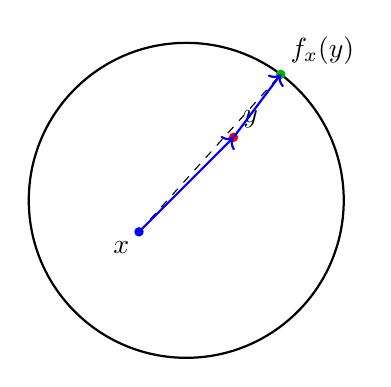
\begin{tikzpicture}[scale=2]
		% Unit disk
		\draw[thick] (0,0) circle (1);
		
		% Points
		\coordinate (X) at (-0.3,-0.2);
		\coordinate (Y) at (0.3,0.4);
		\coordinate (F) at (0.6,0.8); % intersection on boundary (approximate)
		
		% Lines
		\draw[dashed] (X) -- (F);
		
		% Points drawn
		\fill[blue] (X) circle (0.03);
		\fill[red] (Y) circle (0.03);
		\fill[green!70!black] (F) circle (0.03);
		
		% Labels
		\node[below left] at (X) {$x$};
		\node[above right] at (Y) {$y$};
		\node[above right] at (F) {$f_x(y)$};
		
		% Arrow for extension
		\draw[->,thick,blue] (X) -- (Y);
		\draw[->,thick,blue] (Y) -- (F);
		
	\end{tikzpicture}
	\caption{Geometric construction of $f_x(y)$: extend the ray from $x$ through $y$ until it hits the boundary $\partial D$.}
\end{figure}

\section*{Problem 7 (ii)}
With $f_x : K \to \partial D$ defined as above, prove that if $K$ is connected, then $f_x(K)$ is connected in $\partial D$.

\section*{Solution}
By part (i), $f_x$ is continuous. Since $K$ is connected, its continuous image $f_x(K)$ must also be connected. 

As $\partial D$ is the unit circle, the connected subsets of $\partial D$ are either single points or arcs of the circle. Hence $f_x(K)$ is connected in $\partial D$. \qed

\section*{Example}
If $K$ is a line segment inside $D$ not containing $x$, then $f_x(K)$ is the arc of the circle that subtends the segment with respect to $x$.  
If $K=D\setminus \{x\}$, then $f_x(K)=\partial D$.

\begin{figure}[h]
	\centering
	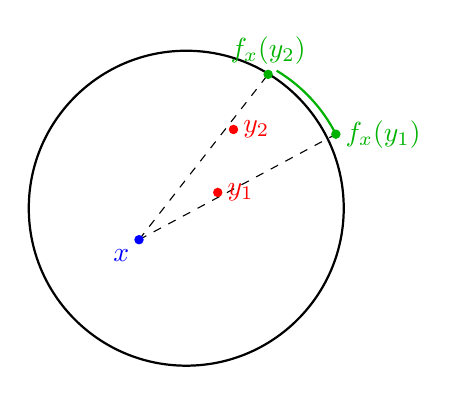
\begin{tikzpicture}[scale=2]
		% Unit circle
		\draw[thick] (0,0) circle (1);
		
		% Points inside
		\coordinate (X) at (-0.3,-0.2);
		\coordinate (A) at (0.2,0.1);
		\coordinate (B) at (0.3,0.5);
		
		% Images on boundary (approximate positions)
		\coordinate (FA) at (0.95,0.47);
		\coordinate (FB) at (0.52,0.85);
		
		% Draw rays
		\draw[dashed] (X) -- (FA);
		\draw[dashed] (X) -- (FB);
		
		% Fill points
		\fill[blue] (X) circle (0.03) node[below left]{$x$};
		\fill[red] (A) circle (0.03) node[right]{$y_1$};
		\fill[red] (B) circle (0.03) node[right]{$y_2$};
		\fill[green!70!black] (FA) circle (0.03) node[right]{$f_x(y_1)$};
		\fill[green!70!black] (FB) circle (0.03) node[above]{$f_x(y_2)$};
		
		% Arc between FA and FB
		\draw[thick,green!70!black] (FA) arc[start angle=27,end angle=59,radius=1];
	\end{tikzpicture}
	\caption{If $K$ is connected (here, a line segment), then $f_x(K)$ is a connected arc of $\partial D$.}
\end{figure}

\section*{Problem 7}
(i) Let $x$ be a point in the closed unit disc $D=\{z\in\mathbb{R}^2 : \|z\|\leq 1\}$, let $K\subseteq D$ be compact not containing $x$, and define $f_x:K\to \partial D$ as follows: for $y\in K$, take the line segment from $x$ to $y$ and extend it until it first hits the boundary $\partial D$. Call this point $f_x(y)$. Prove that $f_x$ is continuous.  

(ii) Show that if $K$ is connected, then $f_x(K)$ is connected in $\partial D$.  

---

\section*{Solution (i)}
For $y\in K$, consider the ray
\[
\ell(t) = x + t(y-x), \quad t\geq 0.
\]
We want $\|\ell(t)\|=1$, i.e.
\[
\|x+t(y-x)\|^2=1.
\]
Solving for $t$ gives
\[
\lambda(y) = \frac{-\langle x, y-x \rangle + \sqrt{\langle x,y-x\rangle^2 + \|y-x\|^2(1-\|x\|^2)}}{\|y-x\|^2}.
\]
Thus
\[
f_x(y) = x + \lambda(y)(y-x).
\]
The denominator $\|y-x\|^2>0$ since $y\neq x$, and the square root is continuous. Therefore $\lambda(y)$ is continuous, hence $f_x$ is continuous. \qed

---

\section*{Solution (ii)}
By part (i), $f_x$ is continuous. Since $K$ is connected, its continuous image $f_x(K)$ must also be connected.  
As $\partial D$ is the unit circle, the connected subsets of $\partial D$ are either single points or arcs. Therefore $f_x(K)$ is connected in $\partial D$. \qed

---

\section*{Examples}
\begin{enumerate}
	\item If $x=0$ (the center of the disc), then
	\[
	f_0(y) = \frac{y}{\|y\|},
	\]
	the usual radial projection onto $\partial D$, which is continuous.
	\item If $K$ is a line segment not containing $x$, then $f_x(K)$ is an arc of $\partial D$.
	\item If $K = D\setminus\{x\}$, then $f_x(K)=\partial D$.
\end{enumerate}

---

\section*{Illustrations}

\begin{figure}[h]
	\centering
	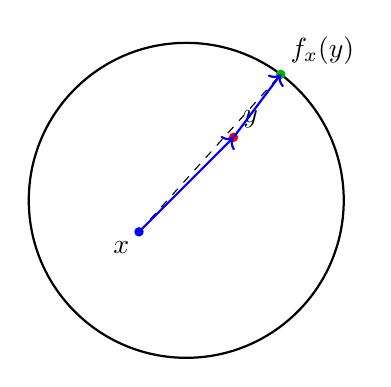
\begin{tikzpicture}[scale=2]
		% Unit disk
		\draw[thick] (0,0) circle (1);
		
		% Points
		\coordinate (X) at (-0.3,-0.2);
		\coordinate (Y) at (0.3,0.4);
		\coordinate (F) at (0.6,0.8); % intersection on boundary (approximate)
		
		% Lines
		\draw[dashed] (X) -- (F);
		
		% Points drawn
		\fill[blue] (X) circle (0.03);
		\fill[red] (Y) circle (0.03);
		\fill[green!70!black] (F) circle (0.03);
		
		% Labels
		\node[below left] at (X) {$x$};
		\node[above right] at (Y) {$y$};
		\node[above right] at (F) {$f_x(y)$};
		
		% Arrow for extension
		\draw[->,thick,blue] (X) -- (Y);
		\draw[->,thick,blue] (Y) -- (F);
		
	\end{tikzpicture}
	\caption{Part (i): $f_x(y)$ is defined by extending the ray from $x$ through $y$ until it hits $\partial D$.}
\end{figure}

\begin{figure}[h]
	\centering
	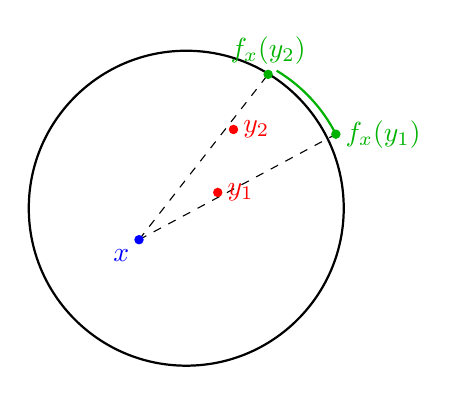
\begin{tikzpicture}[scale=2]
		% Unit circle
		\draw[thick] (0,0) circle (1);
		
		% Points inside
		\coordinate (X) at (-0.3,-0.2);
		\coordinate (A) at (0.2,0.1);
		\coordinate (B) at (0.3,0.5);
		
		% Images on boundary (approximate positions)
		\coordinate (FA) at (0.95,0.47);
		\coordinate (FB) at (0.52,0.85);
		
		% Draw rays
		\draw[dashed] (X) -- (FA);
		\draw[dashed] (X) -- (FB);
		
		% Fill points
		\fill[blue] (X) circle (0.03) node[below left]{$x$};
		\fill[red] (A) circle (0.03) node[right]{$y_1$};
		\fill[red] (B) circle (0.03) node[right]{$y_2$};
		\fill[green!70!black] (FA) circle (0.03) node[right]{$f_x(y_1)$};
		\fill[green!70!black] (FB) circle (0.03) node[above]{$f_x(y_2)$};
		
		% Arc between FA and FB
		\draw[thick,green!70!black] (FA) arc[start angle=27,end angle=59,radius=1];
	\end{tikzpicture}
	\caption{Part (ii): If $K$ is connected (here, a line segment), then $f_x(K)$ is a connected arc on $\partial D$.}
\end{figure}

\section*{Problem 8}
Let $A$ be a $3\times 3$ matrix with positive entries. Use Brouwer's fixed-point theorem to prove that $A$ has an eigenvector with positive entries. 

\section*{Background}
\textbf{Brouwer Fixed-Point Theorem.}  
Every continuous function $f$ from a compact convex subset of $\mathbb{R}^n$ to itself has a fixed point.

\medskip
We apply this to the simplex
\[
T = \{(x_1,x_2,x_3)\in\mathbb{R}^3 : x_i \geq 0,\; x_1+x_2+x_3=1\}.
\]
$T$ is compact and convex, with vertices $(1,0,0),(0,1,0),(0,0,1)$.

\section*{Solution}
Define for $x \in T$:
\[
F(x) = \frac{Ax}{\|Ax\|_1}, \quad \text{where } \|z\|_1 = z_1+z_2+z_3.
\]
Since $A$ has positive entries and $x\in T$ has nonnegative coordinates, $Ax$ has positive coordinates.  
Normalizing ensures $F(x)\in T$, and $F$ is continuous.  

By Brouwer’s theorem, $F$ has a fixed point $x^*\in T$, i.e.
\[
F(x^*) = x^*.
\]
That is,
\[
\frac{Ax^*}{\|Ax^*\|_1} = x^*.
\]
So
\[
Ax^* = \lambda x^*, \quad \text{with } \lambda = \|Ax^*\|_1>0.
\]
Hence $x^*$ is a positive eigenvector of $A$.

\section*{Examples}
\begin{enumerate}
	\item $A=\begin{bmatrix}1&1&1\\1&1&1\\1&1&1\end{bmatrix}$:  
	$F(x)=(1/3,1/3,1/3)$, fixed point is $(1/3,1/3,1/3)$ with eigenvalue $3$.
	\item $A=\begin{bmatrix}1&2&3\\4&5&6\\7&8&9\end{bmatrix}$:  
	$F$ has a positive fixed point $x^*$, corresponding to the Perron eigenvector.
\end{enumerate}

\section*{Connection}
This is an application of the \emph{Perron--Frobenius theorem}: every strictly positive matrix has a positive eigenvector corresponding to its largest eigenvalue.

\section*{Problem 9}
Use the Brouwer fixed-point theorem to prove that there is a complex number $z$ with $|z|\leq 1$ such that
\[
z^4 - z^3 + 8z^2 + 11z + 1 = 0.
\]

\section*{Solution}
\textbf{Step 1. Rearrangement.}  
The equation can be rewritten as
\[
z = \frac{z^4 + 8z^2 + 1}{z^3 - 11}.
\]
Define
\[
F(z) = \frac{z^4 + 8z^2 + 1}{z^3 - 11}.
\]
Then a fixed point of $F$ is a solution of the polynomial equation.

\medskip

\textbf{Step 2. $F$ maps the unit disc to itself.}  
For $|z|\leq 1$,
\[
|z^4 + 8z^2 + 1| \leq 1 + 8 + 1 = 10, \quad
|z^3 - 11| \geq 11 - 1 = 10.
\]
Hence
\[
|F(z)| \leq \frac{10}{10} = 1.
\]
So $F(D) \subseteq D$, where $D=\{z\in\mathbb{C}:|z|\leq 1\}$.

\medskip

\textbf{Step 3. Apply Brouwer.}  
$D$ is compact and convex in $\mathbb{R}^2$, and $F$ is continuous on $D$.  
By Brouwer’s fixed-point theorem, $F$ has a fixed point $z^* \in D$.  
This $z^*$ satisfies
\[
F(z^*) = z^*,
\]
which is equivalent to
\[
(z^*)^4 - (z^*)^3 + 8(z^*)^2 + 11z^* + 1 = 0.
\]

\medskip
\textbf{Conclusion.}  
There exists at least one root of the polynomial inside the closed unit disc $|z|\leq 1$.
\qed

\section*{Problem 10}
Let $C[0,1]$ be the metric space of continuous functions $f:[0,1]\to\mathbb{R}$ with the distance
\[
d(f,g) = \sup_{x\in[0,1]} |f(x)-g(x)|.
\]

\subsection*{(i)}
For $f,g\in C[0,1]$, consider $h(x)=|f(x)-g(x)|$.  
$h$ is continuous on the compact set $[0,1]$, so by the Weierstrass theorem it attains its maximum.  
Thus
\[
d(f,g)=\max_{x\in[0,1]}|f(x)-g(x)|.
\]

\subsection*{(ii)}
Let $X=\{f\in C[0,1]: f(x)\in[0,1]\ \forall x\in[0,1]\}$.  
Consider the sequence $f_n(x)=x^n$. Then $f_n\in X$.  

Pointwise, $f_n(x)\to f(x)$ where
\[
f(x)=\begin{cases}
	0 & 0\leq x<1,\\
	1 & x=1.
\end{cases}
\]
This limit function is not continuous. Hence the sequence cannot converge uniformly in $C[0,1]$.  

Moreover, any subsequence $(f_{n_k})$ has the same pointwise limit, so no subsequence converges uniformly to a continuous function.  
Thus $X$ is not sequentially compact.

\subsection*{(iii)}
Since compactness and sequential compactness are equivalent in metric spaces, $X$ is not compact.  

Explicit open cover: For each $n\in\mathbb{N}$, define
\[
U_n=\{f\in X : f(1) > 1 - \tfrac{1}{n}\}.
\]
Also let
\[
V=\{f\in X : f(1)<1\}.
\]
Then $\{V\}\cup\{U_n: n\in\mathbb{N}\}$ is an open cover of $X$.  

The constant function $f(x)=1$ belongs only to the sets $U_n$, and to cover it one needs infinitely many such $U_n$. Hence there is no finite subcover.  

Therefore $X$ is not compact.
\qed

\section*{Problem 11}
Suppose $f:\mathbb{R}\to\mathbb{R}$ has the intermediate value property (IVP): if $a,b\in\mathbb{R}$ and $f(a)<c<f(b)$, then there exists $y\in(a,b)$ with $f(y)=c$.

\subsection*{(i)}
\textbf{Claim:} $f$ need not be continuous.  

\textbf{Counterexample.} Define
\[
f(x)=\begin{cases}
	\sin\!\left(\tfrac{1}{x}\right), & x\neq 0,\\
	0, & x=0.
\end{cases}
\]
This function has the IVP (as it is a derivative on $\mathbb{R}\setminus\{0\}$), but is not continuous at $0$.  
Thus the IVP does not imply continuity.

\subsection*{(ii)}
Now assume additionally that $f^{-1}(q)$ is closed for every $q\in\mathbb{Q}$.  

Suppose, for contradiction, that $f$ is not continuous at some $x_0$.  
Then there exists $\varepsilon>0$ and a sequence $x_n\to x_0$ with $|f(x_n)-f(x_0)|>\varepsilon$.  

By the IVP, between $f(x_0)$ and $f(x_n)$ the function takes all intermediate values, hence in particular some rational $q$.  
Thus there exist points arbitrarily close to $x_0$ with $f(x)=q$.  
Therefore $x_0$ is a limit point of $f^{-1}(q)$.  
Since $f^{-1}(q)$ is closed, $x_0\in f^{-1}(q)$, i.e.\ $f(x_0)=q$.  

Repeating this with infinitely many different rationals leads to a contradiction.  
Hence $f$ must be continuous at $x_0$.  

\textbf{Conclusion.} With the closed-preimage assumption, $f$ is continuous everywhere.
\qed

\section*{Problem 12}
Let $q\geq 2$ and $n\geq 1$. Define
\[
\mathcal{G}(\{x_1,\dots,x_q\}, \{y_1,\dots,y_q\})
= \inf \left\{ \Big(\sum_{j=1}^q |y_j - x_{\sigma(j)}|^2 \Big)^{1/2} : \sigma \text{ a permutation} \right\}.
\]

\subsection*{(i) $\mathcal{G}$ is a metric.}
\begin{itemize}
	\item Non-negativity: sums of squares are nonnegative.
	\item Identity: $\mathcal{G}(X,Y)=0$ iff $X=Y$ as multisets.
	\item Symmetry: follows since $|y_j-x_{\sigma(j)}|=|x_{\sigma(j)}-y_j|$.
	\item Triangle inequality: For $X,Y,Z$, by Minkowski’s inequality,
	\[
	\Big(\sum_j |x_{\sigma(j)}-z_j|^2\Big)^{1/2}
	\leq \Big(\sum_j |x_{\sigma(j)}-y_{\tau(j)}|^2\Big)^{1/2} + \Big(\sum_j |y_{\tau(j)}-z_j|^2\Big)^{1/2}.
	\]
	Taking infima over permutations $\sigma,\tau$ proves the inequality.
\end{itemize}
Hence $\mathcal{G}$ is a metric on $Q$.

\subsection*{(ii) The case $n=1$.}
If $x_1\leq \dots \leq x_q$ and $y_1\leq \dots \leq y_q$, then by the rearrangement inequality the permutation minimizing
\[
\sum_{j=1}^q (x_{\sigma(j)}-y_j)^2
\]
is the identity permutation. Hence
\[
\mathcal{G}(\{x_1,\dots,x_q\}, \{y_1,\dots,y_q\})
= \Big(\sum_{j=1}^q (x_j-y_j)^2\Big)^{1/2}.
\]

\subsection*{Examples}
\begin{itemize}
	\item $X=\{0,1\}, Y=\{2,3\}$: $\mathcal{G}(X,Y)=\sqrt{8}$.
	\item $X=\{0,2\}, Y=\{1,3\}$: $\mathcal{G}(X,Y)=\sqrt{2}$.
\end{itemize}
\qed


\section*{Problem 12}
Let $q\ge 2$, $n\ge 1$, and $Q$ be the set of unordered $q$-tuples (multisets) of points in $\mathbb{R}^n$.
For $X=\{x_1,\dots,x_q\}$ and $Y=\{y_1,\dots,y_q\}$ define
\[
\mathcal{G}(X,Y)=\inf_{\sigma\in S_q}
\Big(\sum_{j=1}^q \|y_j-x_{\sigma(j)}\|^2\Big)^{1/2}.
\]

\subsection*{(i) $\mathcal{G}$ is a metric on $Q$}
It is permutation-invariant (hence well-defined on multisets), nonnegative and symmetric.
If $\mathcal{G}(X,Y)=0$ there exists $\sigma$ with $\|y_j-x_{\sigma(j)}\|=0$ for all $j$, so $X=Y$ as multisets. Conversely, $X=Y \Rightarrow \mathcal{G}(X,Y)=0$.
For the triangle inequality, for any $\sigma,\pi\in S_q$ and any $X,Y,Z$,
\[
\begin{aligned}
	\Big(\sum_{j}\|x_{\sigma(j)}-z_{\pi(j)}\|^2\Big)^{1/2}
	&=\Big(\sum_{j}\|(x_{\sigma(j)}-y_j)+(y_j-z_{\pi(j)})\|^2\Big)^{1/2}\\
	&\le \Big(\sum_{j}\|x_{\sigma(j)}-y_j\|^2\Big)^{1/2}
	+ \Big(\sum_{j}\|y_j-z_{\pi(j)}\|^2\Big)^{1/2}.
\end{aligned}
\]
Taking infima over $\sigma,\pi$ yields $\mathcal{G}(X,Z)\le \mathcal{G}(X,Y)+\mathcal{G}(Y,Z)$.
Hence $\mathcal{G}$ is a metric.

\subsection*{(ii) The case $n=1$ with sorted labels}
Assume $x_1\le\cdots\le x_q$ and $y_1\le\cdots\le y_q$. If a permutation $\sigma$ has a crossing (i.e.\ $i<k$ but $\sigma(i)>\sigma(k)$), then
\[
(x_i-y_{\sigma(i)})^2+(x_k-y_{\sigma(k)})^2
-(x_i-y_{\sigma(k)})^2-(x_k-y_{\sigma(i)})^2
=2(x_k-x_i)\big(y_{\sigma(i)}-y_{\sigma(k)}\big)\ge0,
\]
so swapping these two pairs does not increase the cost. Iterating removes all crossings; the minimum is attained at the identity permutation. Thus
\[
\mathcal{G}(\{x_1,\dots,x_q\},\{y_1,\dots,y_q\})
=\Big(\sum_{j=1}^q (x_j-y_j)^2\Big)^{1/2}.
\]

\begin{figure}[h]
	\centering
	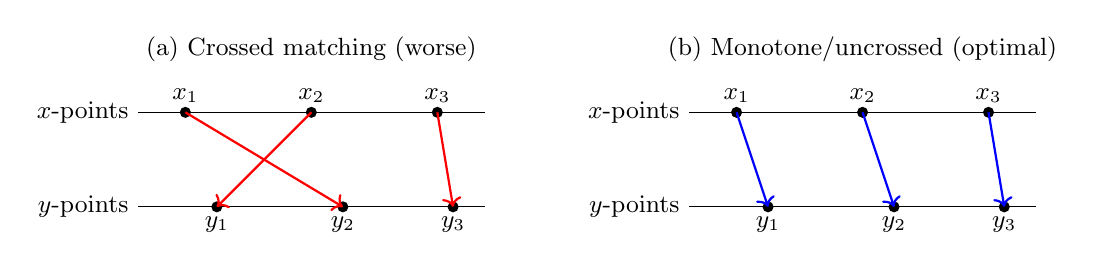
\begin{tikzpicture}[scale=1, every node/.style={font=\small}]
		%---------------- LEFT: CROSSED MATCHING ----------------
		\begin{scope}[xshift=0cm]
			\node at (2.0,2.0) {(a) Crossed matching (worse)};
			% lines for X-row (top) and Y-row (bottom)
			\draw (-0.2,1.2) -- (4.2,1.2);
			\draw (-0.2,0.0) -- (4.2,0.0);
			\node[left] at (-0.2,1.2) {$x$-points};
			\node[left] at (-0.2,0.0) {$y$-points};
			
			% positions (sorted left->right)
			\coordinate (x1) at (0.4,1.2);
			\coordinate (x2) at (2.0,1.2);
			\coordinate (x3) at (3.6,1.2);
			
			\coordinate (y1) at (0.8,0.0);
			\coordinate (y2) at (2.4,0.0);
			\coordinate (y3) at (3.8,0.0);
			
			% points
			\foreach \P/\N in {x1/$x_1$,x2/$x_2$,x3/$x_3$} {
				\fill (\P) circle (2pt) node[above] {\N};
			}
			\foreach \P/\N in {y1/$y_1$,y2/$y_2$,y3/$y_3$} {
				\fill (\P) circle (2pt) node[below] {\N};
			}
			
			% crossed matching: x1->y2, x2->y1, x3->y3
			\draw[->,thick,red] (x1) -- (y2);
			\draw[->,thick,red] (x2) -- (y1);
			\draw[->,thick,red] (x3) -- (y3);
		\end{scope}
		
		%---------------- RIGHT: UNCROSSED MATCHING ----------------
		\begin{scope}[xshift=7cm]
			\node at (2.0,2.0) {(b) Monotone/uncrossed (optimal)};
			% lines
			\draw (-0.2,1.2) -- (4.2,1.2);
			\draw (-0.2,0.0) -- (4.2,0.0);
			\node[left] at (-0.2,1.2) {$x$-points};
			\node[left] at (-0.2,0.0) {$y$-points};
			
			% same positions
			\coordinate (x1) at (0.4,1.2);
			\coordinate (x2) at (2.0,1.2);
			\coordinate (x3) at (3.6,1.2);
			
			\coordinate (y1) at (0.8,0.0);
			\coordinate (y2) at (2.4,0.0);
			\coordinate (y3) at (3.8,0.0);
			
			% points
			\foreach \P/\N in {x1/$x_1$,x2/$x_2$,x3/$x_3$} {
				\fill (\P) circle (2pt) node[above] {\N};
			}
			\foreach \P/\N in {y1/$y_1$,y2/$y_2$,y3/$y_3$} {
				\fill (\P) circle (2pt) node[below] {\N};
			}
			
			% monotone matching: xj -> yj
			\draw[->,thick,blue] (x1) -- (y1);
			\draw[->,thick,blue] (x2) -- (y2);
			\draw[->,thick,blue] (x3) -- (y3);
		\end{scope}
	\end{tikzpicture}
	\caption{In 1D, uncrossing reduces (or keeps) the sum of squared distances. The optimal matching pairs the sorted lists coordinatewise.}
\end{figure}

\section*{Problem}
$p(z)=z^2-4z+3$, $\gamma(t)=p(2e^{2\pi it})$. Show $\gamma$ avoids $0$ and compute $w(\gamma,0)$ in three ways.

\subsection*{Avoiding $0$}
Let $\theta=2\pi t$ and $w=e^{i\theta}$. Then $\gamma(t)=4w^2-8w+3$. If $\gamma(t)=0$,
$4w^2-8w+3=0$ so $w\in\{\tfrac12,\tfrac32\}$, not on $|w|=1$. Hence $\gamma$ does not pass through $0$.

\subsection*{(i) Direct analysis}
$\gamma=4e^{2i\theta}-8e^{i\theta}+3$, so
\[
\Re\gamma=8\cos^2\theta-8\cos\theta-1,\qquad
\Im\gamma=8\sin\theta(\cos\theta-1).
\]
Thus $\Im\gamma=0$ at $\theta=0,\pi$ with $\gamma(0)=-1$ (downward crossing) and $\gamma(\pi)=15$ (upward crossing).
The curve crosses the positive real axis exactly once upward, so the argument increases by $2\pi$ and
$w(\gamma,0)=1$.

\subsection*{(ii) Factoring / argument principle}
$p(z)=(z-1)(z-3)$ has one zero ($z=1$) inside $|z|<2$ and one outside. The argument principle yields
\[
w(\gamma,0)=\#\{\text{zeros of }p \text{ in }|z|<2\}=1.
\]

\subsection*{(iii) Dog-walking lemma}
Let $\alpha(\theta)=2e^{i\theta}-1$ and $\beta(\theta)=2e^{i\theta}-3$. Then $w(\alpha,0)=1$ (circle radius $2$ centered at $-1$
encloses $0$) and $w(\beta,0)=0$ (radius $2$ centered at $-3$ does not). Since $w(\alpha\beta,0)=w(\alpha,0)+w(\beta,0)$,
we obtain $w(\gamma,0)=1$.
\qed

\section*{2. Fixed and antipodal points for extendable maps $S^1\to S^1$}

Let $g:S^1\to S^1$ be continuous and suppose $g$ extends to a continuous
$G:\overline{D}\to S^1$ with $G|_{S^1}=g$.

\medskip

\noindent\textbf{Degree zero / continuous argument.}
Define the homotopy $\Gamma:[0,1]\times[0,2\pi]\to S^1$ by
\[
\Gamma(r,t)=G\!\left(r\,e^{it}\right).
\]
Then $\Gamma(1,t)=g(e^{it})$ and $\Gamma(0,t)\equiv G(0)$ is constant.
Hence the loop $t\mapsto g(e^{it})$ is null-homotopic and has winding number (degree) $0$.
Equivalently, there exists a continuous lift $\phi:[0,2\pi]\to\mathbb{R}$ such that
\[
g(e^{it})=e^{i\phi(t)}\quad\text{and}\quad \phi(2\pi)=\phi(0).
\]

\medskip

\noindent\textbf{Define } $h(t)=\phi(t)-t$. Then $h$ is continuous and
\[
h(2\pi)=\phi(2\pi)-2\pi=\phi(0)-2\pi=h(0)-2\pi.
\]
By the intermediate value theorem, the interval $\big[h(2\pi),h(0)\big]$ (of length $2\pi$)
contains both $0$ and $\pi$ as values of $h$. Hence there exist $t_0,t_1\in[0,2\pi]$ with
\[
h(t_0)=0 \quad\text{and}\quad h(t_1)=\pi.
\]
These equalities mean
\[
\phi(t_0)=t_0 \;\Rightarrow\; g(e^{it_0})=e^{it_0}, \qquad
\phi(t_1)=t_1+\pi \;\Rightarrow\; g(e^{it_1})=-\,e^{it_1}.
\]

\medskip

\noindent\textbf{Conclusion.}
(a) There exists $z_0=e^{it_0}\in S^1$ with $g(z_0)=z_0$.
(b) There exists $z_1=e^{it_1}\in S^1$ with $g(z_1)=-z_1$.
\qed

\section*{3. Uniform approximation by polynomials and discontinuities}

\textbf{Claim.} There is no function $f:[0,1]\to\mathbb{R}$ with a discontinuity that can be approximated
\emph{uniformly} on $[0,1]$ by polynomials.

\textbf{Proof.}
Suppose, to the contrary, there exist polynomials $(p_n)$ with
\[
\|f-p_n\|_\infty=\sup_{x\in[0,1]} |f(x)-p_n(x)| \xrightarrow[n\to\infty]{} 0.
\]
Each $p_n$ is continuous on $[0,1]$, and a uniform limit of continuous functions is continuous.
Hence $f$ must be continuous on $[0,1]$, contradicting the assumption that $f$ has a discontinuity.
Therefore no such $f$ exists. \qed

\medskip
\textbf{Remark.} By the Weierstrass approximation theorem, polynomials are dense in $C[0,1]$
with respect to $\|\cdot\|_\infty$, so uniform polynomial approximation characterizes precisely the
continuous functions on $[0,1]$.

\section*{4. Degrees of uniform polynomial approximants must diverge}

Let $f:[0,1]\to\mathbb{R}$ be continuous and not a polynomial. Suppose $p_n$ are polynomials with
$\|f-p_n\|_\infty\to0$, and write $d_n=\deg p_n$. Then $d_n\to\infty$.

\begin{proof}
	For each $N\in\mathbb{N}$ let
	\[
	\mathcal P_N=\{p\in C[0,1]: p \text{ is a polynomial with } \deg p\le N\}.
	\]
	$\mathcal P_N$ is finite-dimensional, hence a closed subspace of the Banach space $(C[0,1],\|\cdot\|_\infty)$.
	
	Assume for contradiction that $(d_n)$ does not tend to $\infty$. Then there is $N$ and an infinite subsequence $(p_{n_k})$ with $p_{n_k}\in\mathcal P_N$ for all $k$. Since $p_{n_k}\to f$ uniformly and $\mathcal P_N$ is closed, we must have $f\in\mathcal P_N$, i.e.\ $f$ is a polynomial of degree $\le N$, contradicting the hypothesis.
	
	Hence no such $N$ exists, and therefore $d_n\to\infty$.
\end{proof}

\section*{5. Interpolation remainder and uniform convergence}

Let $f:[-1,1]\to\mathbb R$ be $(n\!+\!1)$-times continuously differentiable and
$J_n=\{x_0,\dots,x_n\}\subset[-1,1]$ be $n\!+\!1$ distinct points. Let $P_{J_n}$
be the degree-$\le n$ interpolant with $P_{J_n}(x_j)=f(x_j)$, and set
\[
\beta_{J_n}(x)=\prod_{j=0}^{n}(x-x_j).
\]

\subsection*{(a) Error formula}
For each $x\in[-1,1]$ there exists $\zeta\in(-1,1)$ such that
\[
f(x)-P_{J_n}(x)=\frac{f^{(n+1)}(\zeta)}{(n+1)!}\,\beta_{J_n}(x).
\]
\begin{proof}
	If $x=x_k$ both sides are $0$. Otherwise choose $\lambda$ so that
	$g(y)=f(y)-P_{J_n}(y)-\lambda\,\beta_{J_n}(y)$ satisfies $g(x)=0$.
	Since $g(x_j)=0$ for $j=0,\dots,n$, $g$ has $n\!+\!2$ distinct zeros.
	By repeated Rolle's theorem there exists $\zeta$ with
	$g^{(n+1)}(\zeta)=0$. But
	$g^{(n+1)}(y)=f^{(n+1)}(y)-(n+1)!\lambda$, hence
	$\lambda=\frac{f^{(n+1)}(\zeta)}{(n+1)!}$. Evaluating $g(x)=0$ gives the formula.
\end{proof}

\subsection*{(b) Uniform convergence under a derivative bound}
Assume $f\in C^\infty[-1,1]$ and there exists $M>0$ with
$\sup_{x\in[-1,1]}|f^{(n)}(x)|\le M^n$ for all $n\ge1$.
Then for arbitrary node sets $J_n\subset[-1,1]$,
the interpolants $P_{J_n}$ converge uniformly to $f$ on $[-1,1]$.
\begin{proof}
	By (a),
	\[
	|f(x)-P_{J_n}(x)|\le \frac{\sup_\zeta |f^{(n+1)}(\zeta)|}{(n+1)!}\,|\beta_{J_n}(x)|
	\le \frac{M^{n+1}}{(n+1)!}\,(2)^{n+1},
	\]
	since $|x-x_j|\le 2$ for $x,x_j\in[-1,1]$. The bound tends to $0$ as $n\to\infty$,
	so the convergence is uniform.
\end{proof}

\paragraph{Examples.}
For $f(x)=\sin x$, $\|f-P_{J_n}\|_\infty\le 2^{n+1}/(n+1)!$.
For $f(x)=e^x$ on $[-1,1]$, $\|f-P_{J_n}\|_\infty\le (2e)^{n+1}/(n+1)!$.

\section*{5. Lagrange interpolation error and a uniform convergence criterion}

Let $f:[-1,1]\to\mathbb{R}$ be $(n\!+\!1)$-times continuously differentiable and let
$J_n=\{x_0,\dots,x_n\}\subset[-1,1]$ be distinct nodes. Denote by $P_{J_n}$ the degree-$\le n$
interpolant ($P_{J_n}(x_j)=f(x_j)$), and set
\[
\beta_{J_n}(x)=\prod_{j=0}^{n}(x-x_j).
\]

\subsection*{(a) Remainder formula}
For each $x\in[-1,1]$ there exists $\zeta\in(-1,1)$ such that
\[
f(x)-P_{J_n}(x)=\frac{f^{(n+1)}(\zeta)}{(n+1)!}\,\beta_{J_n}(x).
\]
\begin{proof}
	If $x$ is one of the nodes, both sides vanish. Otherwise define
	$g(y)=f(y)-P_{J_n}(y)-\lambda\,\beta_{J_n}(y)$ and choose $\lambda$ so that $g(x)=0$.
	Then $g(x_j)=0$ for $j=0,\dots,n$, so $g$ has $n\!+\!2$ distinct zeros. By Rolle's theorem
	applied $n\!+\!1$ times, there is $\zeta$ with $g^{(n+1)}(\zeta)=0$. Since
	$g^{(n+1)}(y)=f^{(n+1)}(y)-(n+1)!\lambda$, we obtain
	$\lambda=\frac{f^{(n+1)}(\zeta)}{(n+1)!}$. Evaluating $g(x)=0$ yields the claimed formula.
\end{proof}

\subsection*{(b) Uniform convergence for arbitrary nodes}
Assume $f\in C^\infty[-1,1]$ and there exists $M>0$ with
$\sup_{x\in[-1,1]}|f^{(n)}(x)|\le M^n$ for all $n\ge1$.
Then the interpolants $P_{J_n}$ (for any choice of nodes $J_n$) converge uniformly to $f$ on $[-1,1]$.
\begin{proof}
	From (a) and $|x-x_j|\le2$ for $x,x_j\in[-1,1]$,
	\[
	\|f-P_{J_n}\|_\infty
	\le \frac{\sup_\zeta|f^{(n+1)}(\zeta)|}{(n+1)!}\,\sup_{x\in[-1,1]}|\beta_{J_n}(x)|
	\le \frac{M^{n+1}}{(n+1)!}\,2^{\,n+1}\xrightarrow{n\to\infty}0.
	\]
\end{proof}

\paragraph{Remarks.}
1. The identity in (a) is the Lagrange form of the error; equivalently
$f(x)-P_{J_n}(x)=f[x_0,\dots,x_n,x]\;\beta_{J_n}(x)$, where the divided difference equals
$f^{(n+1)}(\zeta)/(n+1)!$ for some $\zeta$.
2. The hypothesis $\sup|f^{(n)}|\le M^n$ (no factorial) holds for many entire functions with
uniformly bounded derivatives on $[-1,1]$ (e.g.\ $\sin x$, $e^{ax}$ with $M$ chosen large enough).
3. Interpolation can diverge for some analytic $f$ and bad nodes (Runge phenomenon). Part (b) avoids
this by a factorial-over-power bound that beats any node placement.

\paragraph{Rolle's theorem.}
If $f$ is continuous on $[a,b]$, differentiable on $(a,b)$, and $f(a)=f(b)$, then
$\exists\,c\in(a,b)$ with $f'(c)=0$.

\paragraph{Lagrange mean value theorem.}
If $f$ is continuous on $[a,b]$ and differentiable on $(a,b)$, then
$\exists\,c\in(a,b)$ with $f'(c)=\dfrac{f(b)-f(a)}{b-a}$.

\paragraph{Taylor with Lagrange remainder.}
If $f\in C^{n+1}([a,b])$, then for each $x\in[a,b]$ there exists $\xi$ between $a$ and $x$ such that
\[
f(x)=\sum_{k=0}^{n}\frac{f^{(k)}(a)}{k!}(x-a)^k+\frac{f^{(n+1)}(\xi)}{(n+1)!}(x-a)^{n+1}.
\]

\paragraph{Interpolation remainder (Lagrange form).}
With nodes $x_0,\dots,x_n$ and interpolant $P_{J_n}$, for each $x\in[-1,1]$ there exists $\zeta\in(-1,1)$ with
\[
f(x)-P_{J_n}(x)=\frac{f^{(n+1)}(\zeta)}{(n+1)!}\,\prod_{j=0}^{n}(x-x_j).
\]

\section*{6. Minimax node polynomial and Chebyshev nodes}

Let $x_1,\dots,x_n\in[-1,1]$ be distinct and $\beta_J(x)=\prod_{k=1}^n(x-x_k)$.
Define $F(x_1,\dots,x_n)=\sup_{x\in[-1,1]}|\beta_J(x)|$.

\paragraph{Chebyshev background.}
Write $T_n(\cos\theta)=\cos(n\theta)$.
Then $|T_n(x)|\le1$ on $[-1,1]$, $T_n(\cos(j\pi/n))=(-1)^j$ for $j=0,\dots,n$,
the zeros are $\cos\!\big(\frac{(2k-1)\pi}{2n}\big)$ ($k=1,\dots,n$), and
$T_n(x)=2^{n-1}x^n+\cdots$ ($n\ge1$).
Thus the monic Chebyshev is $\widehat T_n(x)=2^{1-n}T_n(x)$ with
$\|\widehat T_n\|_{\infty,[-1,1]}=2^{1-n}$.

\paragraph{Minimax property.}
For any monic polynomial $p$ of degree $n$, put $M=\|p\|_{\infty,[-1,1]}$ and
$R(x)=\widehat T_n(x)-p(x)$ (degree $\le n-1$).
At the points $x_j=\cos(j\pi/n)$ we have
$\widehat T_n(x_j)=2^{1-n}(-1)^j$ and $|p(x_j)|\le M$.
If $M<2^{1-n}$ then $R(x_j)$ alternates sign, so by IVT $R$ has at least $n$
distinct zeros in $(-1,1)$—impossible since $\deg R\le n-1$.
Hence $M\ge2^{1-n}$, with equality precisely for $p=\widehat T_n$.

\paragraph{Conclusion.}
Each $\beta_J$ is monic degree $n$, so
\[
F(x_1,\dots,x_n)=\|\beta_J\|_{\infty,[-1,1]}\ge2^{1-n}.
\]
Equality holds iff $\beta_J=\widehat T_n$, i.e. when
\[
x_k=\cos\!\left(\frac{(2k-1)\pi}{2n}\right),\qquad k=1,\dots,n,
\]
the zeros of $T_n$. Therefore $F$ is minimized at the Chebyshev nodes.
\qed

\paragraph{Chebyshev basics.}
$T_n(\cos\theta)=\cos(n\theta)$; $T_{n+1}=2xT_n-T_{n-1}$; 
$|T_n|\le1$ on $[-1,1]$; zeros at $\cos\frac{(2k-1)\pi}{2n}$.

\paragraph{Minimax.}
Among monic $\deg n$ polynomials, $\min\|p\|_\infty=2^{1-n}$, attained by 
$\widehat T_n=2^{1-n}T_n$ (equioscillation).

\paragraph{Chebyshev series.}
$f(x)\sim \frac{a_0}{2}+\sum_{k\ge1} a_kT_k(x)$,
$a_k=\frac{2}{\pi}\int_{-1}^1\frac{f(x)T_k(x)}{\sqrt{1-x^2}}\,dx$.

\paragraph{Interpolation (barycentric).}
Nodes $x_j=\cos\frac{j\pi}{N}$ give
$p_N(x)=\dfrac{\sum_{j} \frac{w_j f(x_j)}{x-x_j}}{\sum_j \frac{w_j}{x-x_j}}$,
$w_0=w_N=\tfrac12(-1)^j$, $w_j=(-1)^j$.
Lebesgue constant $\Lambda_N=O(\log N)$.

\paragraph{Convergence.}
If $f$ is analytic in Bernstein ellipse $E_\rho$, then $E_n(f)\lesssim C\,\rho^{-n}$.
If $f\in C^r$, then $E_n(f)=O(n^{-r})$.

\section*{1. Chebyshev polynomials $T_n$ (first kind)}
\begin{itemize}[leftmargin=*]
	\item \textbf{Definition via cosine:}
	\[
	T_n(\cos\theta)=\cos(n\theta),\qquad n\ge 0.
	\]
	\item \textbf{Three-term recurrence:}
	\[
	T_0(x)=1,\quad T_1(x)=x,\quad T_{n+1}(x)=2x\,T_n(x)-T_{n-1}(x)\quad (n\ge 1).
	\]
	\item \textbf{Extremal property:} $|T_n(x)|\le 1$ for $x\in[-1,1]$, with
	\[
	T_n\!\Big(\cos\frac{j\pi}{n}\Big)=(-1)^j,\qquad j=0,1,\dots,n.
	\]
	\item \textbf{Zeros:}
	\[
	T_n\!\Big(\cos\frac{(2k-1)\pi}{2n}\Big)=0,\qquad k=1,\dots,n.
	\]
	\item \textbf{Leading coefficient:} for $n\ge 1$,
	\[
	T_n(x)=2^{\,n-1}x^n+\dots
	\]
	\item \textbf{Weighted orthogonality:}
	\[
	\int_{-1}^1 \frac{T_m(x)T_n(x)}{\sqrt{1-x^2}}\,dx=
	\begin{cases}
		0,& m\ne n,\\[2pt]
		\pi,& n=m=0,\\[2pt]
		\frac{\pi}{2},& n=m\ge 1.
	\end{cases}
	\]
\end{itemize}

\section*{2. Minimax (best uniform) monic polynomial}
Let $\widehat T_n(x):=2^{\,1-n}T_n(x)$ (monic, degree $n$). Then
\[
\big\|\widehat T_n\big\|_{\infty,[-1,1]}=\sup_{x\in[-1,1]}\big|\,\widehat T_n(x)\,\big|=2^{\,1-n}.
\]
Moreover, among all monic polynomials $p$ of degree $n$,
\[
\min_{\deg p=n,\ p\text{ monic}}\ \|p\|_{\infty,[-1,1]} \;=\; 2^{\,1-n},
\]
and the unique minimizer is $\widehat T_n$. (Proof idea: alternation at the $n\!+\!1$ points 
$x_j=\cos(j\pi/n)$ and an IVT degree argument.)

\section*{3. Chebyshev nodes and interpolation}
\begin{itemize}[leftmargin=*]
	\item \textbf{Interpolation nodes of degree $N$:}
	\[
	x_j=\cos\frac{j\pi}{N},\qquad j=0,1,\dots,N.
	\]
	\item \textbf{Barycentric weights and interpolant (first kind nodes):}
	\[
	w_0=w_N=\frac12(-1)^j,\qquad w_j=(-1)^j\ (1\le j\le N-1),
	\]
	\[
	p_N(x)=\frac{\displaystyle\sum_{j=0}^{N}\frac{w_j f(x_j)}{x-x_j}}
	{\displaystyle\sum_{j=0}^{N}\frac{w_j}{x-x_j}},\qquad x\notin\{x_j\},\quad p_N(x_j)=f(x_j).
	\]
	\item \textbf{Lebesgue constant:} 
	\[
	\Lambda_N=\sup_{x\in[-1,1]}\sum_{j=0}^N |\ell_j(x)| 
	\sim \frac{2}{\pi}\log N + \mathcal O(1),
	\]
	so Chebyshev interpolation is near-best in the uniform norm.
\end{itemize}

\section*{4. Chebyshev series (orthogonal expansion)}
If $f\in L^2\!\big([-1,1],(1-x^2)^{-1/2}\big)$ then
\[
f(x)\sim \frac{a_0}{2}+\sum_{k=1}^{\infty} a_k T_k(x),\qquad
a_k=\frac{2}{\pi}\int_{-1}^{1}\frac{f(x)T_k(x)}{\sqrt{1-x^2}}\,dx.
\]
For continuous $f$, partial sums (and Fej\'er averages) converge uniformly on $[-1,1]$.

\section*{5. Bernstein ellipse and geometric convergence}
\paragraph{Ellipse.} For $\rho>1$, the Bernstein ellipse $E_\rho$ is the image of the circle $|z|=\rho$ under
\[
x=\frac12\left(z+z^{-1}\right).
\]
It has semi-axes $\frac12(\rho+\rho^{-1})$ and $\frac12(\rho-\rho^{-1})$.

\paragraph{Coefficient decay via a 3-line derivation.}
Define $F(z):=f\!\big(\tfrac12(z+z^{-1})\big)$. If $f$ is analytic and $|f|\le M$ on $E_\rho$, then
$F$ is analytic in the annulus $\rho^{-1}<|z|<\rho$ and bounded by $M$ on $|z|=\rho$.
Using $T_k(x)=\frac12(z^k+z^{-k})$ one finds Chebyshev coefficients are Laurent coefficients of $F$,
and Cauchy's estimate gives
\[
|a_k|\le \frac{2M}{\rho^k},\qquad k\ge 0.
\]

\paragraph{Best polynomial and interpolant error bounds.}
Let $E_n(f)=\min_{\deg p\le n}\|f-p\|_{\infty,[-1,1]}$. If $f$ is analytic and $|f|\le M$ on $E_\rho$,
then
\[
E_n(f)\ \le\ \frac{2M}{\rho^n(\rho-1)}.
\]
Furthermore, Chebyshev \emph{interpolation} of degree $N$ obeys
\[
\|f-p_N\|_{\infty,[-1,1]}\ \le\ C\,\frac{M}{\rho^N(\rho-1)},
\]
with a modest absolute constant $C$ (e.g.\ $C=4$ from a simple tail bound). In particular, the error decays
geometrically like $\rho^{-N}$.

\section*{6. Interpolation remainder (Lagrange form)}
For distinct nodes $x_0,\dots,x_n$ and $f\in C^{n+1}([-1,1])$, with 
$\displaystyle \beta_{J_n}(x)=\prod_{j=0}^{n}(x-x_j)$, there exists $\zeta\in(-1,1)$ such that
\[
f(x)-P_{J_n}(x)=\frac{f^{(n+1)}(\zeta)}{(n+1)!}\,\beta_{J_n}(x).
\]
Consequently, since $|x-x_j|\le 2$ on $[-1,1]$,
\[
\|f-P_{J_n}\|_{\infty,[-1,1]}\ \le\ \frac{\sup_{[-1,1]}|f^{(n+1)}|}{(n+1)!}\,2^{\,n+1}.
\]
If $\sup_{[-1,1]}|f^{(k)}|\le M^k$ for all $k$, the right-hand side $\to 0$ (factorial beats power).

\section*{7. Mapping to a general interval $[a,b]$}
Use the affine map
\[
x=\frac{2t-(b+a)}{b-a},\qquad t\in[a,b].
\]
Nodes become
\[
t_j=\frac{a+b}{2}+\frac{b-a}{2}\cos\frac{j\pi}{N},\qquad j=0,\dots,N,
\]
and all bounds on $[-1,1]$ carry over to $[a,b]$ under this map.

\section*{8. Practical recipe (spectral accuracy for analytic $f$)}
\begin{enumerate}[leftmargin=*]
	\item Map your interval to $[-1,1]$.
	\item Sample $f$ at Chebyshev nodes $x_j=\cos\frac{j\pi}{N}$.
	\item Form the interpolant via the barycentric formula (or compute Chebyshev coefficients using a DCT / Clenshaw--Curtis).
	\item Evaluate with the barycentric form or Clenshaw's recurrence for stability.
	\item Expect $\|f-p_N\|_\infty\approx \mathrm{const}\cdot \rho^{-N}$, where $\rho$ is determined by the distance of the nearest complex singularity (Bernstein ellipse touching it).
\end{enumerate}

\section*{9. Tiny worked examples}
\begin{itemize}[leftmargin=*]
	\item \textbf{$f(x)=\sin x$ (entire).} For any $\rho>1$ the assumptions hold, so errors decay faster than $c\,\rho^{-N}$ for every $\rho$; practically, near machine precision with modest $N$.
	\item \textbf{$f(x)=\dfrac{1}{1+25x^2}$.} Singularities at $\pm i/5$; choose $\rho$ so the Bernstein ellipse passes through $i/5$. Then $E_n(f)\lesssim C\,\rho^{-n}$; interpolation at Chebyshev nodes enjoys the same geometric rate.
	\item \textbf{$f(x)=|x|$.} Not analytic; Chebyshev coefficients satisfy $a_{2m}\sim \mathcal O(m^{-2})$ and $a_{2m+1}=0$, hence best and interpolant errors behave like $c\,N^{-2}$ (algebraic decay). A Gibbs-type kink remains near $0$.
\end{itemize}



\section*{1. Setting and notation}
Let \(C([0,1])\) be the real Banach space of continuous functions on \([0,1]\) with the uniform norm
\[
\norm{h}_\infty := \sup_{x\in[0,1]} \lvert h(x)\rvert .
\]
For a fixed positive integer \(n\), write
\[
\Pspace := \{\, p : \text{$p$ is a polynomial with }\deg p < n \,\},
\]
a finite–dimensional subspace of \(C([0,1])\).

\paragraph{Best (minimax) approximant.}
Given \(f\in C([0,1])\), a polynomial \(p^\ast\in \Pspace\) is called a
\emph{best uniform approximant (of degree \(<n\))} if
\[
\norm{f-p^\ast}_\infty = \inf_{q\in \Pspace} \norm{f-q}_\infty .
\]
We denote the minimal error by
\[
E^\ast_n(f) := \inf_{q\in \Pspace} \norm{f-q}_\infty .
\]

\paragraph{Existence (why a minimizer exists).}
Since \(\Pspace\) is finite–dimensional, all norms are equivalent on it.
If \(\norm{p}_\infty > 2\norm{f}_\infty\) then by the triangle inequality
\(\norm{f-p}_\infty \ge \norm{p}_\infty - \norm{f}_\infty > \norm{f}_\infty\),
so such \(p\) cannot beat the zero polynomial.
Therefore the minimization can be restricted to the closed ball
\(\{p\in \Pspace : \norm{p}_\infty \le 2\norm{f}_\infty\}\), which is compact in finite dimension.
The map \(p \mapsto \norm{f-p}_\infty\) is continuous; hence a minimizer exists.

\section*{2. Haar systems, alternation, and the Chebyshev norm}
The family \(\{1,x,x^2,\dots,x^{n-1}\}\) forms a \emph{Haar system} on \([0,1]\): no nontrivial linear combination
has more than \(n-1\) zeros unless it vanishes identically. Equivalently, every nonzero \(p\in \Pspace\)
has at most \(n-1\) distinct zeros. This fact underlies the sign–change arguments below.

The uniform norm is \emph{convex but not strictly convex}; consequently, best approximants need not be unique
in general spaces. The Haar property, together with the alternation principle, restores uniqueness here.

\section*{3. de la Vallée Poussin lower bound}
\begin{lemma}[de la Vallée Poussin]\label{dlVP}
	Let \(f\in C([0,1])\), \(p\in \Pspace\), and suppose there exist points
	\(0\le a_0<\cdots<a_m\le 1\) with \(m\ge n\) such that
	\[
	f(a_k)-p(a_k) = (-1)^k \alpha \qquad (k=0,\dots,m)
	\]
	for some \(\alpha>0\). Then for every \(q\in \Pspace\),
	\[
	\norm{f-q}_\infty \ge \alpha .
	\]
\end{lemma}

\begin{proof}[Idea]
	Put \(r=q-p\in \Pspace\). At the alternation points,
	\[
	(-1)^k\big(f(a_k)-q(a_k)\big) = \alpha - (-1)^k r(a_k).
	\]
	If \(\norm{f-q}_\infty<\alpha\), then the left side has absolute value \(<\alpha\) for all \(k\),
	forcing \((-1)^k r(a_k)>0\) for each \(k\). Thus \(r(a_k)\) alternates sign,
	so \(r\) has at least \(m\ge n\) distinct zeros, impossible for \(\deg r< n\) unless \(r\equiv 0\).
	In that case \(\norm{f-q}_\infty = \norm{f-p}_\infty = \alpha\).
\end{proof}

\section*{4. Equioscillation (equal–ripple) criterion}
\begin{theorem}[Chebyshev equioscillation; necessity and sufficiency]\label{alternation}
	Let \(f\in C([0,1])\) and \(n\ge 1\). A polynomial \(p\in \Pspace\) is a best uniform approximant if and only if
	there exist \(n+1\) points \(0\le a_0<\cdots<a_n\le 1\) such that
	\[
	f(a_k)-p(a_k) = (-1)^k \norm{f-p}_\infty \qquad (k=0,\dots,n),
	\]
	or the same with \((-1)^{k+1}\).
\end{theorem}

\begin{proof}[Sketch]
	Necessity can be proved by a perturbation argument.
	Sufficiency follows from Lemma~\ref{dlVP} with \(\alpha=\norm{f-p}_\infty\) and \(m=n\).
\end{proof}

\section*{5. Uniqueness of the minimizer}
\begin{theorem}[Uniqueness]\label{uniq}
	For each \(f\in C([0,1])\) and each integer \(n\ge 1\), the minimizer \(p^\ast\in \Pspace\)
	of \(\norm{f-p}_\infty\) is unique.
\end{theorem}

\begin{proof}
	Let \(p,q\in \Pspace\) be minimizers with the same minimal error \(E\).
	By Theorem~\ref{alternation} applied to \(p\), choose \(0\le a_0<\cdots<a_n\le 1\) with
	\(f(a_k)-p(a_k)=(-1)^k E\). Let \(r:=p-q\in \Pspace\). At each \(a_k\),
	\[
	(-1)^k r(a_k) = -E + (-1)^k\big(f(a_k)-q(a_k)\big) \le 0 .
	\]
	Thus on each interval \([a_k,a_{k+1}]\) either \(r\) vanishes or changes sign.
	So \(r\) has at least \(n\) distinct zeros, forcing \(r\equiv 0\) because \(\deg r< n\).
	Thus \(p\equiv q\).
\end{proof}


\section*{Pointwise polynomial approximation on \(\mathbb{R}\)}
\paragraph{Theorem.}
If \(f:\mathbb{R}\to\mathbb{R}\) is continuous, then there exist polynomials \(p_n\) such that
\(p_n(x)\to f(x)\) for every \(x\in\mathbb{R}\).

\paragraph{Proof.}
Fix \(n\in\mathbb{N}\). The restriction \(f|_{[-n,n]}\) is continuous on the compact interval \([-n,n]\).
By the Weierstrass approximation theorem, there exists a polynomial \(p_n\) with
\[
\sup_{|x|\le n}\,|f(x)-p_n(x)|<\frac{1}{n}.
\tag{$\ast$}
\]
Now fix \(x\in\mathbb{R}\) and choose \(N\) so that \(|x|\le N\).
For all \(n\ge N\), inequality \((\ast)\) applies at the point \(x\), hence
\[
|p_n(x)-f(x)|\le \frac{1}{n}\xrightarrow[n\to\infty]{}0.
\]
Therefore \(p_n(x)\to f(x)\) for every \(x\in\mathbb{R}\).
\qed

\section*{Weierstrass Approximation Theorem}

\paragraph{Setting.}
Let \(C([a,b])\) denote the space of real continuous functions on \([a,b]\) with the uniform norm
\[
\norm{f}_\infty=\sup_{x\in[a,b]} |f(x)|.
\]

\begin{theorem}[Weierstrass]
	For every \(f\in C([a,b])\) and every \(\varepsilon>0\) there exists a polynomial \(p\) such that
	\[
	\sup_{x\in[a,b]} |f(x)-p(x)|<\varepsilon.
	\]
	Equivalently, polynomials are dense in \(C([a,b])\) with respect to \(\norm{\cdot}_\infty\).
\end{theorem}

\paragraph{Constructive proof on \([0,1]\) (Bernstein polynomials).}
For \(n\in\mathbb N\) and \(x\in[0,1]\), define
\[
B_n(f,x)=\sum_{k=0}^{n} f\!\left(\tfrac{k}{n}\right)\binom{n}{k} x^{k}(1-x)^{n-k}.
\]
Then \(B_n(f,\cdot)\) is a polynomial. Using the probabilistic identity
\[
B_n(f,x)=\mathbb E\!\left[f\!\left(\tfrac{S_n}{n}\right)\right],\qquad S_n\sim\mathrm{Bin}(n,x),
\]
together with \(\mathbb E[S_n/n]=x\) and \(\mathrm{Var}(S_n/n)=x(1-x)/n\), and writing
\(\omega_f(\delta)=\sup_{|u-v|\le \delta}|f(u)-f(v)|\) (modulus of continuity), one obtains
\[
|B_n(f,x)-f(x)|\le \omega_f\!\left(\sqrt{\frac{x(1-x)}{n}}\right)\le \omega_f\!\left(\frac{1}{2\sqrt{n}}\right).
\]
Hence \(\norm{B_n(f)-f}_\infty\to0\) as \(n\to\infty\).
For a general interval \([a,b]\), compose with the affine map \([a,b]\leftrightarrow[0,1]\).

\paragraph{Stone--Weierstrass (context).}
More generally, if \(K\) is compact and \(\mathcal A\subset C(K)\) is a subalgebra that separates points and contains constants,
then \(\mathcal A\) is dense in \(C(K)\). Taking \(K=[a,b]\) and \(\mathcal A\) the algebra of polynomials yields Weierstrass.

\paragraph{Corollary (pointwise approximation on \(\mathbb R\)).}
If \(f:\mathbb R\to\mathbb R\) is continuous, then there exist polynomials \(p_n\) with
\(\sup_{|x|\le n}|f(x)-p_n(x)|<1/n\). For any fixed \(x\), this implies \(p_n(x)\to f(x)\) as \(n\to\infty\).

\section*{Bernstein operator: direct uniform convergence for \(f(x)=x^3\)}

\paragraph{Definition.}
For \(f\in C[0,1]\), the Bernstein polynomial is
\[
(B_n f)(x)=\sum_{k=0}^n f\!\left(\frac{k}{n}\right)\binom{n}{k}x^{k}(1-x)^{n-k},\qquad x\in[0,1].
\]
Equivalently, if \(S_n\sim\mathrm{Bin}(n,x)\), then \((B_n f)(x)=\mathbb E\!\left[f(S_n/n)\right]\).

\paragraph{Computation for \(f(x)=x^3\).}
Using the factorial-moment identity \(S^3=(S)_3+3(S)_2+(S)_1\) and
\(\mathbb E[(S_n)_r]=n^{\underline r}x^r\) with \(n^{\underline r}=n(n-1)\cdots(n-r+1)\),
\[
B_n(x^3)(x)=\frac{n^{\underline 3}x^3+3n^{\underline 2}x^2+n x}{n^3}
= x^3 + \frac{3x^2-3x^3}{n} + \frac{x-3x^2+2x^3}{n^2}.
\]
Hence
\[
B_n(x^3)(x)-x^3=\frac{3x^2(1-x)}{n}+\frac{x(1-x)(1-2x)}{n^2}.
\]

\paragraph{Uniform bound.}
On \([0,1]\), \(0\le x^2(1-x)\le \tfrac{4}{27}\) and \(|x(1-x)(1-2x)|\le \tfrac14\).
Therefore
\[
\sup_{x\in[0,1]} |B_n(x^3)(x)-x^3|
\le \frac{4}{9n}+\frac{1}{4n^2}\xrightarrow[n\to\infty]{}0.
\]
Thus \(B_n f\to f\) uniformly on \([0,1]\) for \(f(x)=x^3\).
\qed

\paragraph{Direct computation from the Bernstein formula (no expectation).}
For \(t\in[0,1]\),
\[
B_n(x^3)(t)=\sum_{k=0}^{n}\left(\frac{k}{n}\right)^3 \binom{n}{k}\, t^{k}(1-t)^{n-k}.
\]
Using \(k^3=(k)_3+3(k)_2+(k)_1\) and the identities
\[
k\binom{n}{k}=n\binom{n-1}{k-1},\quad
k(k-1)\binom{n}{k}=n(n-1)\binom{n-2}{k-2},\quad
k(k-1)(k-2)\binom{n}{k}=n(n-1)(n-2)\binom{n-3}{k-3},
\]
we obtain
\[
\sum_{k=0}^{n} k^3 \binom{n}{k} t^{k}(1-t)^{n-k}
= n(n-1)(n-2)\, t^{3} + 3 n(n-1)\, t^{2} + n\, t.
\]
Dividing by \(n^3\) yields
\[
B_n(x^3)(t)
= t^3 + \frac{3t^2-3t^3}{n} + \frac{t-3t^2+2t^3}{n^2},
\]
so
\[
B_n(x^3)(t)-t^3=\frac{3t^2(1-t)}{n}+\frac{t(1-t)(1-2t)}{n^2}.
\]
Since \(0\le t^2(1-t)\le \tfrac{4}{27}\) and \(|t(1-t)(1-2t)|\le \tfrac14\) on \([0,1]\),
\[
\sup_{t\in[0,1]}|B_n(x^3)(t)-t^3|
\le \frac{4}{9n}+\frac{1}{4n^2}\to 0,
\]
hence \(B_n(x^3)\to x^3\) uniformly on \([0,1]\).
\subsection*{Chebyshev polynomials (first kind)}
They are defined by \(T_n(\cos\theta)=\cos(n\theta)\) and satisfy
\(T_0(x)=1\), \(T_1(x)=x\), and \(T_{n+1}(x)=2x\,T_n(x)-T_{n-1}(x)\).

The first five are
\[
\begin{aligned}
	T_0(x)&=1,\\
	T_1(x)&=x,\\
	T_2(x)&=2x^2-1,\\
	T_3(x)&=4x^3-3x,\\
	T_4(x)&=8x^4-8x^2+1.
\end{aligned}
\]

(Optionally, \(T_5(x)=16x^5-20x^3+5x\).)

\section*{Legendre polynomials: Gram--Schmidt, endpoint vanishing, and Rodrigues-type $P_n$}

\paragraph{Inner product.}
\(\langle f,g\rangle=\displaystyle\int_{-1}^{1} f(x)g(x)\,dx.\)

\subsection*{(i) First four Legendre polynomials via Gram--Schmidt}
\[
p_0(x)=1,\qquad p_1(x)=x,\qquad
p_2(x)=\tfrac12(3x^2-1),\qquad
p_3(x)=\tfrac12(5x^3-3x).
\]
(Outline: orthogonalize \(1,x,x^2,x^3\). Use
\(\langle x,1\rangle=0\),
\(x^2-(\langle x^2,1\rangle/\langle1,1\rangle)=x^2-\tfrac13\),
and
\(x^3-(\langle x^3,x\rangle/\langle x,x\rangle)x=x^3-\tfrac35 x\),
then scale to the standard normalization \(p_n(1)=1\).)

\subsection*{(ii) Endpoint vanishing and orthogonality}
For \(\phi_n(x)=(1-x)^n(1+x)^n=(1-x^2)^n\),
\(x=\pm1\) is a zero of multiplicity \(n\), hence
\[
\frac{d^m}{dx^m}\phi_n(\pm1)=0\quad\text{for all }m<n.
\]
Define \(P_n(x):=\dfrac{d^n}{dx^n}(1-x^2)^n\).
For \(m<n\),
\[
\int_{-1}^{1} P_n(x)P_m(x)\,dx
=\int \phi_n^{(n)}\,\phi_m^{(m)}
=(-1)^n\!\int \phi_n\,\phi_m^{(m+n)}=0,
\]
where we integrated by parts \(n\) times; all boundary terms vanish by the endpoint-vanishing above, and \(\phi_m^{(m+n)}\equiv0\) since \(\deg\phi_m=2m<m+n\).
Hence the \(P_n\) form an orthogonal family of degree \(n\) and therefore are scalar multiples of the Legendre polynomials \(p_n\).

\subsection*{(iii) Computing \(P_n\) for \(n=0,1,2,3\)}
\[
\begin{aligned}
	P_0(x)&=1,\\
	P_1(x)&=-2x=(-2)\,p_1(x),\\
	P_2(x)&=-4+12x^2=8\,p_2(x),\\
	P_3(x)&=72x-120x^3=(-48)\,p_3(x).
\end{aligned}
\]
Thus \(P_n=(-1)^n 2^n n!\,p_n\) for \(n=0,1,2,3\), confirming the conclusion in (ii).


\section*{Moments determine a continuous function}

\paragraph{Claim.}
If \(f\in C[0,1]\) and \(\int_0^1 f(x)x^n\,dx=0\) for all \(n=0,1,2,\dots\), then \(f\equiv0\).
If instead \(\int_0^1 f(x)x^n\,dx=0\) holds for all \(n\ge1\), the same conclusion still holds.

\paragraph{Proof (case \(n\ge0\)).}
Define \(L:C[0,1]\to\mathbb R\) by \(L(g)=\int_0^1 f(x)g(x)\,dx\).
Then \(L\) is continuous and \(L(p)=0\) for every polynomial \(p\).
By the Weierstrass theorem, polynomials are dense in \(C[0,1]\), hence \(L\equiv0\).
Taking \(g=f\) gives \(\int_0^1 f(x)^2\,dx=0\), so \(f\equiv0\).

\paragraph{Proof (case \(n\ge1\) only).}
Again let \(L(g)=\int_0^1 f(x)g(x)\,dx\).
If \(p\) is a polynomial with \(p(0)=0\), then \(p(x)=\sum_{k=1}^m a_k x^k\), so \(L(p)=0\) by hypothesis.
By density of such polynomials in \(\{g\in C[0,1]:g(0)=0\}\), we obtain
\(L(g)=0\) for every continuous \(g\) with \(g(0)=0\).
Therefore, for arbitrary \(\varphi\in C[0,1]\),
\[
L(\varphi)=L\big(\varphi-\varphi(0)\big)+\varphi(0)L(1)=c\,\varphi(0),\qquad c:=\int_0^1 f.
\]
Let \(\varphi_\varepsilon\) be a continuous function with \(\varphi_\varepsilon(0)=1\) and
\(\operatorname{supp}\varphi_\varepsilon\subset[0,\varepsilon]\).
Then
\[
c=L(\varphi_\varepsilon)=\int_0^1 f(x)\varphi_\varepsilon(x)\,dx
\quad\text{and}\quad |L(\varphi_\varepsilon)|\le \|f\|_\infty\,\varepsilon\to0,
\]
hence \(c=0\). Thus \(L(\varphi)=0\) for all \(\varphi\in C[0,1]\), and taking \(\varphi=f\) yields
\(\int_0^1 f(x)^2\,dx=0\). By continuity, \(f\equiv0\).
\qed

\paragraph{Remark.}
Without continuity, the second statement is false: the point mass \(\delta_0\) has
\(\int_0^1 x^n\,d\delta_0=0\) for all \(n\ge1\) but is not the zero function.

\section*{Orthogonalization of \(1,x,x^2,\dots\) on \([-1,1]\) (Legendre via Gram--Schmidt)}

\paragraph{Inner product.}
\(\displaystyle \langle f,g\rangle=\int_{-1}^{1} f(x)g(x)\,dx.\)
Useful integrals: \(\int_{-1}^{1} x^m\,dx=0\) for \(m\) odd, and \(=2/(m+1)\) for \(m\) even.

\paragraph{Results (scaled so \(p_n(1)=1\)).}
\[
\begin{aligned}
	p_0(x)&=1,\\
	p_1(x)&=x,\\
	p_2(x)&=\tfrac12(3x^2-1),\\
	p_3(x)&=\tfrac12(5x^3-3x),\\
	p_4(x)&=\tfrac18(35x^4-30x^2+3).
\end{aligned}
\]

\paragraph{Sketch of Gram--Schmidt steps.}
\[
\begin{aligned}
	&u_0=1\ \Rightarrow\ p_0=1,\\[2pt]
	&u_1=x-\frac{\langle x,1\rangle}{\langle 1,1\rangle}1=x\ \Rightarrow\ p_1=x,\\[2pt]
	&u_2=x^2-\frac{\langle x^2,1\rangle}{\langle 1,1\rangle}1=x^2-\tfrac13\ \Rightarrow\
	p_2=\tfrac32\bigl(x^2-\tfrac13\bigr),\\[2pt]
	&u_3=x^3-\frac{\langle x^3,x\rangle}{\langle x,x\rangle}x=x^3-\tfrac35 x\
	\Rightarrow\ p_3=\tfrac52\bigl(x^3-\tfrac35 x\bigr),\\[2pt]
	&u_4=x^4-\frac{\langle x^4,1\rangle}{\langle 1,1\rangle}1
	-\frac{\langle x^4,p_2\rangle}{\langle p_2,p_2\rangle}p_2
	=x^4-\tfrac{6}{7}x^2+\tfrac{3}{35},\\
	&\hspace{48pt}p_4=\frac{35}{8}\,u_4=\tfrac18(35x^4-30x^2+3).
\end{aligned}
\]

\paragraph{Orthonormal scaling.}
\(\displaystyle \int_{-1}^{1}p_n^2=\frac{2}{2n+1}\), so
\(\displaystyle \phi_n(x)=\sqrt{\frac{2n+1}{2}}\,p_n(x)\) is orthonormal.

\section*{Orthogonality of Chebyshev polynomials and the weight}
Let \(T_n\) be the Chebyshev polynomials of the first kind, defined by \(T_n(\cos\theta)=\cos(n\theta)\).
Set
\[
w(x)=\frac{1}{\sqrt{1-x^2}},\qquad x\in(-1,1).
\]
Then for all \(m,n\ge 0\),
\[
\int_{-1}^{1} T_m(x)\,T_n(x)\,w(x)\,dx
= \int_{-1}^{1} T_m(x)T_n(x)\frac{dx}{\sqrt{1-x^2}}
= \int_{0}^{\pi} \cos(m\theta)\cos(n\theta)\,d\theta,
\]
where we used the substitution \(x=\cos\theta\) (so \(dx=-\sin\theta\,d\theta\) and
\(dx/\sqrt{1-x^2}=-d\theta\)).
By the standard cosine orthogonality on \([0,\pi]\),
\[
\int_{0}^{\pi} \cos(m\theta)\cos(n\theta)\,d\theta=
\begin{cases}
	0, & m\ne n,\\
	\pi, & m=n=0,\\
	\pi/2, & m=n\ge 1.
\end{cases}
\]
Therefore \(\{T_n\}_{n\ge0}\) is an orthogonal system on \([-1,1]\) with respect to
\(w(x)=(1-x^2)^{-1/2}\). An orthonormal system is given by
\[
\phi_0(x)=\frac{1}{\sqrt{\pi}},\qquad
\phi_n(x)=\sqrt{\frac{2}{\pi}}\,T_n(x)\quad(n\ge1).
\]

\section*{Quadrature with nodes and weights; exactness and Gauss rules}

Fix an interval $[a,b]$. For $n\in\mathbb N$, let nodes $x_k^{(n)}\in[a,b]$ and weights $A_k^{(n)}\ge 0$ be given
($k=1,\dots,n$). Define
\[
Q_n(P):=\sum_{k=1}^n A_k^{(n)}\,P\!\bigl(x_k^{(n)}\bigr),\qquad
\varepsilon_n(P):=\left|\int_a^b P(x)\,dx\;-\;Q_n(P)\right|.
\]

\paragraph{Exactness and moment conditions.}
The rule is exact for all polynomials of degree $\le m$ if and only if
\[
\sum_{k=1}^n A_k^{(n)}\bigl(x_k^{(n)}\bigr)^j=\int_a^b x^j\,dx\qquad (j=0,1,\dots,m),
\]
i.e.\ the first $m{+}1$ moments are matched.

\paragraph{Sharp upper bound.}
No $n$-node rule can be exact beyond degree $2n-1$. Indeed, if it were exact for degree $2n$,
then with $\pi(x)=\prod_{k=1}^n(x-x_k^{(n)})^2\ge 0$ we would get
$0=Q_n(\pi)=\sum_{k} A_k^{(n)}\pi(x_k^{(n)})=\int_a^b \pi(x)\,dx>0$, a contradiction.

\paragraph{Gauss--Legendre rule (achieves $2n{-}1$).}
Let $P_n$ be the degree-$n$ Legendre polynomial on $[-1,1]$ and let $\xi_1,\dots,\xi_n$ be its zeros.
Set nodes on $[a,b]$ by $x_k^{(n)}=\frac{a+b}{2}+\frac{b-a}{2}\,\xi_k$ and weights by
\[
A_k^{(n)}=\frac{b-a}{2}\,\omega_k,\qquad
\omega_k=\frac{2}{\bigl(1-\xi_k^2\bigr)\,[P_n'(\xi_k)]^2}\ (>0).
\]
Then
\[
\sum_{k=1}^n A_k^{(n)}\,P\!\bigl(x_k^{(n)}\bigr)=\int_a^b P(x)\,dx
\qquad\text{for all polynomials } \deg P\le 2n-1.
\]
\emph{Sketch:} write $p=qP_n+r$ with $\deg q,\deg r\le n-1$; orthogonality gives $\int qP_n=0$ and
$P_n(\xi_k)=0$ gives $p(\xi_k)=r(\xi_k)$; the quadrature integrates $r$ exactly.

\paragraph{Examples on $[-1,1]$.}
\begin{itemize}
	\item $n=1$: node $0$, weight $2$; exact for $\deg\le 1$.
	\item $n=2$: nodes $\pm 1/\sqrt{3}$, weights $1,1$; exact for $\deg\le 3$.
	\item $n=3$: nodes $0,\ \pm\sqrt{3/5}$; weights $8/9,\ 5/9,\ 5/9$; exact for $\deg\le 5$.
\end{itemize}
Mapping to $[a,b]$ uses $x=\frac{a+b}{2}+\frac{b-a}{2}\xi$ and multiplies all weights by $\frac{b-a}{2}$.

\section*{Function Approximation vs.\ Quadrature (on \([-1,1]\))}

\subsection*{A. Polynomial approximation of a continuous function}
\textbf{Goal.} Given \(f\in C([-1,1])\), choose a polynomial \(p_n\) so that
\[
\|f-p_n\|_\infty=\sup_{x\in[-1,1]} |f(x)-p_n(x)|
\]
is small (ideally, minimal). This targets the \emph{entire function} on the whole interval.

\textbf{Tools.} Weierstrass approximation (existence of good polynomials), Chebyshev
(minimax/near-best choices), Jackson-type estimates (rates in terms of smoothness).

\subsection*{B. Numerical quadrature (this task)}
\textbf{Goal.} Approximate the \emph{single number}
\[
I(f)=\int_{-1}^{1} f(x)\,dx
\]
by a weighted sum of \emph{finitely many samples}:
\[
Q_n(f)=\sum_{k=1}^{n} A_k\,f(x_k),\qquad x_k\in[-1,1],\ A_k>0.
\]
We design \(x_k,A_k\) so that \(Q_n\) is \emph{exact} for all polynomials of degree
\(\le m\):
\[
Q_n(p)=\int_{-1}^{1} p(x)\,dx\quad\text{for all }\deg p\le m.
\]
Any \(n\)-node rule has \(m\le 2n-1\) (sharp). \emph{Gauss--Legendre} quadrature
(zeros of the Legendre polynomial \(P_n\) as nodes, specific positive weights)
achieves \(m=2n-1\).

\subsection*{C. Same actors, different roles}
Orthogonal polynomials appear in both settings:
\begin{itemize}
	\item In \emph{approximation}, expanding \(f\) in Chebyshev/Legendre series and truncating gives small \(\|f-p_n\|_\infty\).
	\item In \emph{quadrature}, Gauss nodes are the zeros of an orthogonal polynomial, yielding exactness up to degree \(2n-1\).
\end{itemize}

\subsection*{D. Tiny example}
For \(f(x)=x^4\) on \([-1,1]\):
\begin{itemize}
	\item A degree-1 polynomial \(p(x)=ax+b\) cannot uniformly approximate \(x^4\) well; the optimal error is \(O(1)\).
	\item The 3-point Gauss rule (degree of exactness \(5\)) integrates \(x^4\) \emph{exactly} using just 3 samples, even though it does not approximate the whole function.
\end{itemize}

\subsection*{E. Side-by-side comparison}
\begin{center}
	\begin{tabular}{|l|l|l|}
		\hline
		\textbf{Aspect} & \textbf{Approximation} & \textbf{Quadrature} \\
		\hline
		Target & \(f(\cdot)\) on \([-1,1]\) & \(\displaystyle \int_{-1}^{1} f\) (a scalar) \\
		\hline
		Output & Polynomial \(p_n\) & Nodes \(x_k\), weights \(A_k\) \\
		\hline
		Error & \(\|f-p_n\|_\infty\) (uniform) & \(\bigl|\int f-\sum A_k f(x_k)\bigr|\) \\
		\hline
		Optimality & Minimax/Chebyshev, etc. & Degree of exactness \(m\le 2n-1\) \\
		\hline
		Data used & Potentially dense info on \(f\) & Only \(n\) samples \(f(x_k)\) \\
		\hline
		Key tools & Weierstrass, Chebyshev series & Orthogonal polys, Gauss nodes \\
		\hline
	\end{tabular}
\end{center}

\section*{No $n$-node quadrature can be exact beyond degree $2n-1$}

Let $\alpha_1,\dots,\alpha_n\in[-1,1]$ be distinct nodes and $A_1,\dots,A_n\in\mathbb R$ weights.
Consider the quadrature $Q_n(p)=\sum_{j=1}^n A_j\,p(\alpha_j)$.

\begin{theorem}
	For any choice of nodes and weights, the degree of exactness of $Q_n$ is at most $2n-1$.
	In particular, there do not exist $n$ distinct nodes and real weights such that
	\[
	\int_{-1}^{1} p(x)\,dx=\sum_{j=1}^n A_j\,p(\alpha_j)
	\quad\text{for all } \deg p\le 2n .
	\]
\end{theorem}

\begin{proof}
	Define $\displaystyle \pi(x)=\prod_{j=1}^n (x-\alpha_j)^2$. Then $\deg\pi=2n$, and $\pi(\alpha_j)=0$ for all $j$,
	so $Q_n(\pi)=0$. Since $\pi\ge 0$ and $\pi\not\equiv 0$, we have $\int_{-1}^1 \pi(x)\,dx>0$.
	If the rule were exact for degree $2n$, we would have $Q_n(\pi)=\int_{-1}^1 \pi$, a contradiction.
	Hence the degree of exactness is $\le 2n-1$.
\end{proof}

\paragraph{Optimality.}
The Gauss--Legendre rule, with nodes the zeros of the Legendre polynomial $P_n$
and the usual positive weights, is exact for all $\deg p\le 2n-1$, so the bound is sharp.

\paragraph{Checks.}
For $n=1$, exactness for $1,x,x^2$ forces $A_1=2$, $\alpha_1=0$, and $2\alpha_1^2=2/3$, impossible.
For $n=2$ with symmetric nodes $\pm c$ and equal weights $w$, exactness for $1,x^2,x^4$ yields
$w=1$, $c^2=1/3$, and $c^4=1/5$, a contradiction.


\section*{What an \(n\)-point quadrature rule means}

\paragraph{Definition.}
An \(n\)-point quadrature rule on \([a,b]\) is specified by \emph{nodes}
\(x_1,\dots,x_n\in[a,b]\) and \emph{weights} \(A_1,\dots,A_n\) and approximates
\[
\int_a^b f(x)\,dx \;\approx\; Q_n(f):=\sum_{k=1}^{n} A_k\,f(x_k).
\]
Thus the rule requires exactly \(n\) function evaluations \(f(x_k)\).

\paragraph{Degree of exactness.}
The rule is \emph{exact of degree \(m\)} if \(Q_n(p)=\int_a^b p(x)\,dx\) for every polynomial
\(p\) with \(\deg p\le m\).
With only function values (no derivatives), any \(n\)-point rule satisfies \(m\le 2n-1\) (sharp).
Gauss--Legendre quadrature attains \(m=2n-1\).

\paragraph{Closed vs.\ open rules.}
Nodes may include endpoints (\emph{closed} rules, e.g.\ trapezoid, Simpson) or avoid them
(\emph{open} rules, e.g.\ midpoint). In either case there are \(n\) nodes and \(n\) evaluations.

\paragraph{Composite/adaptive use.}
To integrate on \([a,b]\) one often partitions the interval and applies the \(n\)-point rule on each
subinterval; the overall method then uses many points (roughly \(n\) times the number of panels),
but per panel it remains an \(n\)-point quadrature.

\paragraph{Examples on \([-1,1]\).}
\begin{itemize}
	\item 2-point Gauss: nodes \(\pm 1/\sqrt{3}\), weights \(1,1\); exact for \(\deg\le 3\).
	\item Simpson’s rule (3 points): nodes \(-1,0,1\), weights \(\tfrac{1}{3}(1,4,1)\); exact for \(\deg\le 3\).
\end{itemize}

\section*{Examples of \(n\)-point quadrature rules and what you evaluate}

\paragraph{Definition.}
An \(n\)-point rule on \([a,b]\) has nodes \(x_1,\dots,x_n\in[a,b]\) and weights
\(A_1,\dots,A_n\) and computes
\[
\int_a^b f(x)\,dx \approx Q_n(f):=\sum_{k=1}^n A_k\,f(x_k),
\]
so you evaluate \(f\) at exactly \(n\) points \(x_k\).

\paragraph{Standard rules (nodes, weights, degree of exactness).}
On \([a,b]\) we have:
\[
\begin{array}{|c|l|l|c|}
	\hline
	\text{Rule} & \text{Nodes } x_k & \text{Weights } A_k & \text{Exact for }\deg\le \\
	\hline
	\text{Midpoint }(n=1) & \frac{a+b}{2} &
	b-a & 1\\
	\hline
	\text{Trapezoid }(n=2) & a,\ b &
	\frac{b-a}{2},\ \frac{b-a}{2} & 1\\
	\hline
	\text{Simpson }(n=3) & a,\ \frac{a+b}{2},\ b &
	\frac{b-a}{6}\cdot(1,4,1) & 3\\
	\hline
	\text{Gauss--Legendre }(n=2) &
	\frac{a+b}{2}\pm \frac{b-a}{2\sqrt{3}} &
	\frac{b-a}{2},\ \frac{b-a}{2} & 3\\
	\hline
	\text{Gauss--Legendre }(n=3) &
	\frac{a+b}{2},\ \frac{a+b}{2}\pm \frac{b-a}{2}\sqrt{\frac{3}{5}} &
	\frac{b-a}{2}\cdot\Big(\frac{8}{9},\frac{5}{9},\frac{5}{9}\Big) & 5\\
	\hline
\end{array}
\]

\paragraph{What you actually compute.}
For example, with the 3-point Gauss rule on \([a,b]\):
\[
Q_3(f)=\frac{b-a}{2}\left[\frac{8}{9}\,f\!\left(\tfrac{a+b}{2}\right)
+\frac{5}{9}\,f\!\left(\tfrac{a+b}{2}-\tfrac{b-a}{2}\sqrt{\tfrac{3}{5}}\right)
+\frac{5}{9}\,f\!\left(\tfrac{a+b}{2}+\tfrac{b-a}{2}\sqrt{\tfrac{3}{5}}\right)\right],
\]
which uses \emph{exactly three} evaluations of \(f\).

\paragraph{Sanity check on \([-1,1]\) for \(f(x)=x^4\) (true integral \(=2/5\)).}
\[
\begin{aligned}
	\text{Simpson: }&\frac{2}{6}\,[f(-1)+4f(0)+f(1)]=\frac{1}{3}(1+0+1)=\frac{2}{3},\\
	\text{Gauss 2-point: }& f(-1/\sqrt3)+f(1/\sqrt3)=2\cdot\left(\frac{1}{\sqrt3}\right)^4=\frac{2}{9},\\
	\text{Gauss 3-point: }& \frac{8}{9}\,f(0)+\frac{5}{9}\,f(\pm\sqrt{3/5})
	=\frac{10}{9}\left(\frac{3}{5}\right)^2=\frac{2}{5}.
\end{aligned}
\]
Only the 3-point Gauss rule (degree \(5\)) integrates the quartic exactly.

\section*{Approximating integrals by exactness on polynomials; Legendre background}

\paragraph{Quadrature and degree of exactness.}
An \(n\)-point rule on \([-1,1]\) has nodes \(x_1,\dots,x_n\) and weights \(A_1,\dots,A_n\) and computes
\[
Q_n(f)=\sum_{k=1}^n A_k f(x_k).
\]
It is \emph{exact of degree \(m\)} if \(Q_n(p)=\int_{-1}^{1}p(x)\,dx\) for every polynomial \(p\) with \(\deg p\le m\).
With \(n\) nodes (no derivatives) one always has \(m\le 2n-1\) (sharp).

\paragraph{Legendre polynomials.}
They form an orthogonal basis on \([-1,1]\) (weight \(1\)):
\[
\int_{-1}^{1}P_n(x)P_m(x)\,dx=\begin{cases}\dfrac{2}{2n+1},&m=n,\\[4pt]0,&m\ne n.\end{cases}
\]
Rodrigues: \(P_n(x)=\dfrac{1}{2^n n!}\dfrac{d^n}{dx^n}(x^2-1)^n\).
Recurrence: \((n+1)P_{n+1}=(2n+1)xP_n-nP_{n-1}\).

\paragraph{Gauss--Legendre quadrature (achieves \(2n{-}1\)).}
Let \(\xi_1,\dots,\xi_n\) be the zeros of \(P_n\). Set
\[
\omega_k=\frac{2}{(1-\xi_k^2)\,[P_n'(\xi_k)]^2}
\quad(\text{all }\omega_k>0),
\qquad
Q_n(f)=\sum_{k=1}^n \omega_k\,f(\xi_k).
\]
Then \(Q_n(p)=\int_{-1}^{1}p(x)\,dx\) for every \(\deg p\le 2n-1\).
\emph{Sketch:} write \(p=qP_n+r\) with \(\deg q,\deg r\le n-1\); use \(\int qP_n=0\) and \(P_n(\xi_k)=0\), and the fact that \(Q_n\) integrates any degree-\(\le n{-}1\) polynomial exactly.

\paragraph{Examples on \([-1,1]\).}
\begin{itemize}
	\item \(n=2\): nodes \(\pm 1/\sqrt{3}\), weights \(1,1\); exact for \(\deg\le 3\).
	\item \(n=3\): nodes \(0,\ \pm\sqrt{3/5}\), weights \(8/9,\ 5/9,\ 5/9\); exact for \(\deg\le 5\).
\end{itemize}

\paragraph{Impossibility beyond \(2n{-}1\).}
For any nodes \(\{\alpha_j\}\), the polynomial \(\pi(x)=\prod_{j=1}^n(x-\alpha_j)^2\) has degree \(2n\),
satisfies \(Q_n(\pi)=0\), but \(\int_{-1}^{1}\pi(x)\,dx>0\). Hence no \(n\)-point rule can be exact for all \(\deg 2n\) polynomials.

\section*{Building a 10-point quadrature for \([a,b]\)}

\paragraph{Goal.}
Approximate \(\displaystyle I(f)=\int_a^b f(x)\,dx\) from \(n=10\) samples of \(f\).

\subsection*{A. Choosing the nodes (Gauss--Legendre, optimal)}
Let \((\xi_i,\omega_i)\) be the 10-point Gauss--Legendre nodes/weights on \([-1,1]\):
\[
\begin{aligned}
	\xi_{1,10}&=\pm 0.9739065285171717, & \omega_{1,10}&=0.0666713443086881,\\
	\xi_{2,9} &=\pm 0.8650633666889845, & \omega_{2,9} &=0.1494513491505806,\\
	\xi_{3,8} &=\pm 0.6794095682990244, & \omega_{3,8} &=0.2190863625159820,\\
	\xi_{4,7} &=\pm 0.4333953941292472, & \omega_{4,7} &=0.2692667193099963,\\
	\xi_{5,6} &=\pm 0.1488743389816312, & \omega_{5,6} &=0.2955242247147529.
\end{aligned}
\]
Map to \([a,b]\) by
\[
x_i=\frac{a+b}{2}+\frac{b-a}{2}\,\xi_i,\qquad
A_i=\frac{b-a}{2}\,\omega_i,
\]
and compute
\[
Q_{10}(f)=\sum_{i=1}^{10} A_i\,f(x_i).
\]
This rule is exact for all polynomials with \(\deg\le 19\).

\subsection*{B. Nodes are given (interpolatory quadrature)}
Let distinct \(x_1,\dots,x_{10}\in[a,b]\) be given and define the Lagrange basis
\[
\ell_k(x)=\prod_{\substack{j=1\\ j\ne k}}^{10}\frac{x-x_j}{x_k-x_j}.
\]
Set the weights by
\[
A_k=\int_a^b \ell_k(x)\,dx,\qquad k=1,\dots,10.
\]
Then
\[
Q_{10}(f)=\sum_{k=1}^{10} A_k\,f(x_k)
\]
is exact for all polynomials of degree \(\le 9\).
Equivalently, \(\{A_k\}\) solve the moment system
\[
\sum_{k=1}^{10} A_k\,x_k^{\,j}=\frac{b^{j+1}-a^{j+1}}{j+1},\qquad j=0,1,\dots,9.
\]

\paragraph{Remarks.}
(1) Affine-scaling to \([-1,1]\) before forming \(\ell_k\) or the moment system improves conditioning.\\
(2) If the nodes are equally spaced (including endpoints), this yields the closed Newton--Cotes rule with 10 points, which is less stable than Gauss--Legendre.

\section*{Chebyshev tail with nonnegative coefficients: equioscillation of the truncation error}

Let \(T_j\) be the Chebyshev polynomials of the first kind and let \(\{\gamma_j\}_{j\ge1}\) be
nonnegative with \(\sum_{j=1}^\infty \gamma_j<\infty\).
Define
\[
f(x)=\sum_{j=1}^\infty \gamma_j\,T_{3j}(x),\qquad
P_n(x)=\sum_{j=1}^{n} \gamma_j\,T_{3j}(x),\qquad
R_n(x)=f(x)-P_n(x)=\sum_{j=n+1}^\infty \gamma_j\,T_{3j}(x).
\]

\paragraph{(1) Continuity.}
Since \(|T_{3j}(x)|\le 1\) on \([-1,1]\) and \(\sum\gamma_j<\infty\),
the series for \(f\) converges absolutely and uniformly (M–test), so \(f\in C([-1,1])\).

\paragraph{(2) Exact size of the tail.}
For all \(x\in[-1,1]\),
\(|R_n(x)|\le \sum_{j=n+1}^\infty \gamma_j=:E_n\).
At \(x=1\), \(T_{3j}(1)=1\), hence \(|R_n(1)|=E_n\).
Therefore \(\|f-P_n\|_\infty=\|R_n\|_\infty=E_n\).

\paragraph{(3) Minimax property of \(P_n\).}
Let \(\mathcal P_{3n}\) be the polynomials of degree \(\le 3n\).
For any \(Q\in \mathcal P_{3n}\), write \(Q=\sum_{k=0}^{3n} a_k T_k\).
Then
\[
f-Q=\sum_{j=1}^{n}(\gamma_j-a_{3j})T_{3j}
\;+\;\sum_{\substack{0\le k\le 3n\\k\not\equiv 0\,(3)}}(-a_k)T_k
\;+\;R_n .
\]
Using \(\bigl\|\sum c_\ell T_\ell\bigr\|_\infty\le\sum |c_\ell|\) gives
\[
\|f-Q\|_\infty\ \ge\ \|R_n\|_\infty
- \sum_{j=1}^{n}\bigl|\gamma_j-a_{3j}\bigr|
- \sum_{k\not\equiv0(3)}|a_k|
\ \ge\ \|R_n\|_\infty=E_n,
\]
with equality iff \(a_{3j}=\gamma_j\) for \(1\le j\le n\) and \(a_k=0\) for \(k\not\equiv0\pmod3\), i.e.\ iff \(Q=P_n\).
Thus \(P_n\) is the minimax polynomial in \(\mathcal P_{3n}\) and the best error equals \(E_n\).

\paragraph{(4) Equioscillation points.}
By the Chebyshev alternation theorem for best uniform approximation by \(\mathcal P_{3n}\),
there exist points
\[
-1\le x_0<x_1<\cdots<x_{3n+1}\le 1
\]
such that
\[
f(x_k)-P_n(x_k)=(-1)^k\,\|f-P_n\|_\infty
=(-1)^k\sum_{j=n+1}^\infty \gamma_j,\qquad k=0,1,\dots,3n+1.
\]

\section*{Using 10 points to approximate \(\int_a^b f(x)\,dx\)}

\paragraph{Gauss--Legendre (you may choose the points).}
Let \((\xi_i,\omega_i)_{i=1}^{10}\) be the 10-point Gauss–Legendre nodes/weights on \([-1,1]\).
Map to \([a,b]\) by
\[
x_i=\frac{a+b}{2}+\frac{b-a}{2}\,\xi_i,\qquad
A_i=\frac{b-a}{2}\,\omega_i.
\]
Then the quadrature
\[
Q_{10}(f)=\sum_{i=1}^{10} A_i\,f(x_i)
\]
is exact for every polynomial \(p\) with \(\deg p\le 19\) (optimal among all 10-point rules),
and all \(A_i>0\).

\paragraph{Interpolatory rule (points are pre-given).}
If distinct \(x_1,\dots,x_{10}\in[a,b]\) are given, define the Lagrange basis
\[
\ell_k(x)=\prod_{\substack{j=1\\ j\ne k}}^{10}\frac{x-x_j}{x_k-x_j},
\qquad
A_k=\int_a^b \ell_k(x)\,dx.
\]
Then
\[
Q_{10}(f)=\sum_{k=1}^{10} A_k\,f(x_k)
\]
is exact for all polynomials with \(\deg\le 9\).
(Equivalently, the weights solve \(\sum_{k=1}^{10} A_k x_k^{\,j}=(b^{j+1}-a^{j+1})/(j+1)\) for \(j=0,\dots,9\).)

\section*{Problem 4}
For each \(f\in C([-1,1])\), let \(\mathcal P_n\) denote the subspace of polynomials of degree
at most \(n\), and define the best uniform approximation error
\[
E_n(f):=\inf_{p\in \mathcal P_n}\ \sup_{x\in[-1,1]} |f(x)-p(x)|.
\]
By the Weierstrass approximation theorem, \(E_n(f)\to 0\) for every \(f\in C([-1,1])\).
Using the result of Question~3, construct a function \(f\in C([-1,1])\) to show that the
convergence \(E_n(f)\to 0\) can be \emph{arbitrarily slow} in the following sense:

\medskip
\noindent
\textbf{Claim to prove.} For any decreasing sequence \((\delta_n)_{n\ge1}\) of nonnegative numbers with
\(\delta_n\to 0\), there exists \(f\in C([-1,1])\) such that
\[
E_n(f)\ \ge\ \delta_n \qquad\text{for all } n=1,2,\dots.
\]

\section*{Arbitrarily slow uniform polynomial approximation}

For \(f\in C([-1,1])\) let
\[
E_n(f):=\inf_{p\in\mathcal P_n}\ \|f-p\|_\infty,\qquad
\mathcal P_n=\{p:\deg p\le n\}.
\]
By Weierstrass, \(E_n(f)\downarrow 0\). We show the convergence can be arbitrarily slow.

\paragraph{Lemma (from Problem 3).}
If \(\gamma_j\ge0\) with \(\sum_{j=1}^\infty\gamma_j<\infty\) and
\[
f(x)=\sum_{j=1}^\infty \gamma_j\,T_{3j}(x),\qquad
P_n(x)=\sum_{j=1}^{n}\gamma_j\,T_{3j}(x),
\]
then \(f\in C([-1,1])\), \(P_n\) is the best uniform approximant of degree \(\le 3n\), and
\[
E_{3n}(f)=\|f-P_n\|_\infty=\sum_{j=n+1}^\infty \gamma_j.
\]

\paragraph{Theorem (arbitrarily slow decay of \(E_n(f)\)).}
Given any decreasing sequence \(\delta_n\ge0\) with \(\delta_n\to 0\), there exists
\(f\in C([-1,1])\) such that \(E_n(f)\ge \delta_n\) for all \(n\ge1\).

\begin{proof}
	Set \(s_n:=\delta_{3n}\) and define \(\gamma_{n+1}:=s_n-s_{n+1}\ge0\).
	Then \(\sum \gamma_j=s_0-\lim s_n<\infty\) and hence
	\(f(x):=\sum_{j=1}^\infty \gamma_j T_{3j}(x)\in C([-1,1])\).
	By the lemma,
	\[
	E_{3n}(f)=\sum_{j=n+1}^\infty\gamma_j=s_n=\delta_{3n}.
	\]
	Since \(E_n(f)\) is nonincreasing in \(n\), for any \(m\in\{3n,3n+1,3n+2\}\),
	\[
	E_m(f)\ge E_{3n}(f)=\delta_{3n}\ge \delta_m,
	\]
	because \(\delta_n\) is decreasing. Therefore \(E_n(f)\ge \delta_n\) for all \(n\).
\end{proof}

\paragraph{Examples.}
Choosing \(\delta_n=1/\log(n+e)\) (or \(1/\log\log(n+e^e)\), etc.) yields a continuous \(f\)
for which \(E_n(f)\) decreases as slowly as the prescribed sequence.

\section*{Piecewise-linear (hat-function) interpolation on a uniform grid}

\paragraph{Definition.}
For $n\in\mathbb N$ and $r\in\mathbb Z$, define
\[
\Delta_{n,r}(x):=\max\!\Big\{0,\; 1-n\bigl|x-\tfrac{r}{n}\bigr|\Big\},\qquad x\in[-1,1].
\]
Each $\Delta_{n,r}$ is the “hat” centered at $r/n$ with height $1$ and support
$\big[(r-1)/n,\,(r+1)/n\big]$.

\paragraph{Sketch.}
$\Delta_{n,r}$ is triangular: it is linear on $[(r-1)/n,r/n]$ and on $[r/n,(r+1)/n]$, with
\[
\Delta_{n,r}(r/n)=1,\qquad \Delta_{n,r}((r\pm1)/n)=0.
\]
For fixed $x$, at most two hats are nonzero and they satisfy
$\sum_{m=-n}^n \Delta_{n,m}(x)=1$.

\paragraph{Interpolator.}
Given $f:[-1,1]\to\mathbb R$, set
\[
f_n(x):=\sum_{m=-n}^{n} f\!\left(\tfrac{m}{n}\right)\,\Delta_{n,m}(x).
\]

\begin{lemma}[Piecewise linearity and interpolation]
	For each $n$, $f_n$ is linear on each subinterval $[r/n,(r+1)/n]$, and
	$f_n(r/n)=f(r/n)$ for $r=-n,\dots,n$.
\end{lemma}

\begin{proof}
	On $[r/n,(r+1)/n]$ only $\Delta_{n,r}$ and $\Delta_{n,r+1}$ are nonzero, both linear, and
	$\Delta_{n,r}(x)+\Delta_{n,r+1}(x)=1$. Hence
	\[
	f_n(x)=\Delta_{n,r}(x)\,f(r/n)+\Delta_{n,r+1}(x)\,f((r+1)/n)
	\]
	is linear there. At $x=r/n$, $\Delta_{n,r}(r/n)=1$ and all other hats vanish, so $f_n(r/n)=f(r/n)$.
\end{proof}

\begin{theorem}[Uniform convergence for continuous data]
	If $f\in C([-1,1])$, then $\|f_n-f\|_\infty\to 0$ as $n\to\infty$.
\end{theorem}

\begin{proof}
	Since $f$ is uniformly continuous, for any $\varepsilon>0$ choose $\delta>0$ so that
	$|f(x)-f(y)|<\varepsilon$ whenever $|x-y|<\delta$. Take $n$ with $1/n<\delta$.
	For $x\in[r/n,(r+1)/n]$,
	\[
	\begin{aligned}
		|f_n(x)-f(x)|
		&=\big|\Delta_{n,r}(x)(f(r/n)-f(x))+\Delta_{n,r+1}(x)(f((r+1)/n)-f(x))\big|\\
		&\le \Delta_{n,r}(x)\,|f(r/n)-f(x)|
		+\Delta_{n,r+1}(x)\,|f((r+1)/n)-f(x)|
		< \varepsilon,
	\end{aligned}
	\]
	since both $|x-r/n|$ and $|x-(r+1)/n|$ are $\le 1/n<\delta$. Taking the supremum over $x$ gives
	$\|f_n-f\|_\infty<\varepsilon$.
\end{proof}

\paragraph{Rate under Lipschitz continuity (optional).}
If $f$ is Lipschitz with constant $L$, then for all $x$,
\[
|f_n(x)-f(x)|\le L\max\big\{|x-r/n|,\ |x-(r+1)/n|\big\}\le \frac{L}{n},
\]
hence $\|f_n-f\|_\infty\le L/n$.


% ---------- FIGURE A: hat (tent) functions ----------
\begin{figure}[h]
	\centering
	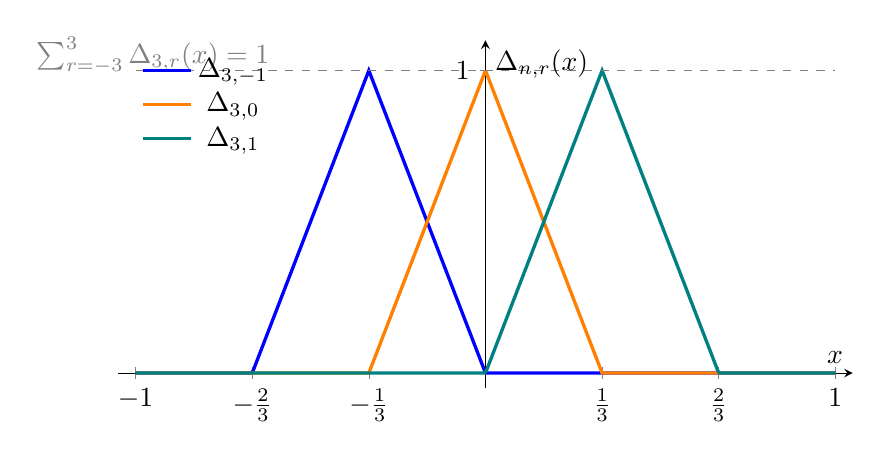
\begin{tikzpicture}
		\begin{axis}[
			width=0.9\linewidth, height=6cm,
			xmin=-1.05, xmax=1.05, ymin=-0.05, ymax=1.1,
			axis lines=middle,
			xlabel={$x$}, ylabel={$\Delta_{n,r}(x)$},
			xtick={-1,-2/3,-1/3,0,1/3,2/3,1},
			xticklabels={$-1$,$-\tfrac{2}{3}$,$-\tfrac{1}{3}$,$0$,$\tfrac{1}{3}$,$\tfrac{2}{3}$,$1$},
			ytick={0,1},
			legend style={at={(0.02,0.98)},anchor=north west,draw=none,fill=none},
			clip=false
			]
			% choose n=3
			\pgfmathsetmacro{\n}{3}
			
			% three hat functions
			\addplot[very thick,blue,domain=-1:1,samples=400] {max(0, 1 - \n*abs(x - (-1)/\n))};
			\addlegendentry{$\Delta_{3,-1}$}
			
			\addplot[very thick,orange,domain=-1:1,samples=400] {max(0, 1 - \n*abs(x - 0/\n))};
			\addlegendentry{$\Delta_{3,0}$}
			
			\addplot[very thick,teal,domain=-1:1,samples=400] {max(0, 1 - \n*abs(x - (1)/\n))};
			\addlegendentry{$\Delta_{3,1}$}
			
			% sum of hats = 1
			\addplot[dashed,gray,domain=-1:1] {1};
			\node[gray] at (axis cs:-0.95,1.05) {$\sum_{r=-3}^{3}\Delta_{3,r}(x)=1$};
		\end{axis}
	\end{tikzpicture}
	\caption{Three neighboring hat functions for $n=3$. Each peak is at $x=r/n$; support width is $2/n$.}
\end{figure}

% ---------- FIGURE B: f vs. piecewise-linear interpolant ----------
\begin{figure}[h]
	\centering
	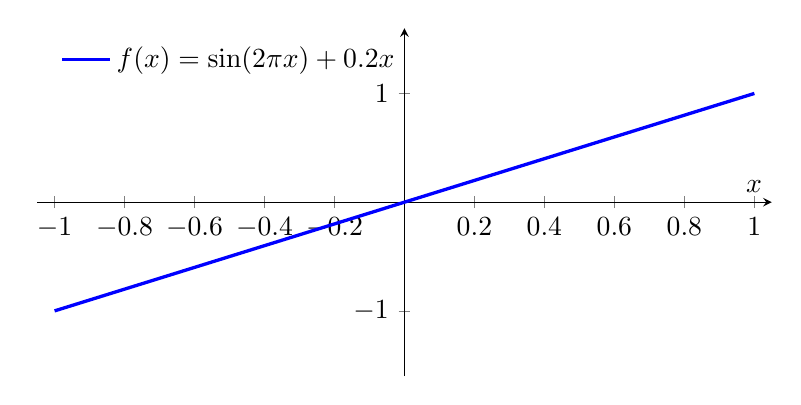
\begin{tikzpicture}
		\begin{axis}[
			width=0.9\linewidth, height=6cm,
			xmin=-1.05, xmax=1.05, ymin=-1.6, ymax=1.6,
			axis lines=middle,
			xlabel={$x$}, ylabel={},
			legend style={at={(0.02,0.98)},anchor=north west,draw=none,fill=none},
			clip=false
			] % <--- THIS closes the axis options correctly
			
			% target function
			\addplot[very thick,blue,domain=-1:1,samples=600] { x};
			\addlegendentry{$f(x)=\sin(2\pi x)+0.2x$}
			
			% piecewise-linear interpolant for n=6
		
			\addlegendentry{$f_n$ (piecewise linear, $n=6$)}
			
		
			
		\end{axis}
	\end{tikzpicture}
	\caption{Piecewise-linear interpolant $f_n$ on a uniform grid with $n=6$.}
\end{figure}


% ---------- FIGURE B: f vs. piecewise-linear interpolant ----------
\begin{figure}[h]
	\centering
	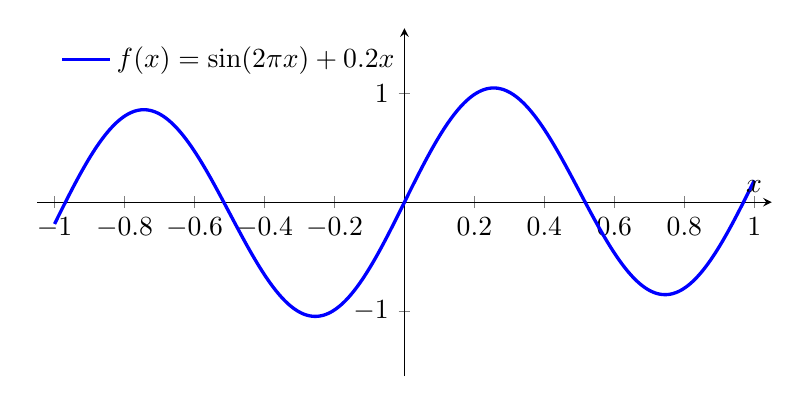
\begin{tikzpicture}
		\begin{axis}[
			width=0.9\linewidth, height=6cm,
			xmin=-1.05, xmax=1.05, ymin=-1.6, ymax=1.6,
			axis lines=middle,
			xlabel={$x$}, ylabel={},
			legend style={at={(0.02,0.98)},anchor=north west,draw=none,fill=none},
			clip=false
			]
			
			% target function f(x) = sin(2πx) + 0.2x
			\addplot[very thick,blue,domain=-1:1,samples=600] {sin(deg(2*pi*x)) + 0.2*x};
			\addlegendentry{$f(x)=\sin(2\pi x)+0.2x$}
			
		\end{axis}
	\end{tikzpicture}
	\caption{Target function $f(x)=\sin(2\pi x)+0.2x$.}
\end{figure}

% ---------- FIGURE B: f vs. piecewise-linear interpolant ----------
\begin{figure}[h]
	\centering
	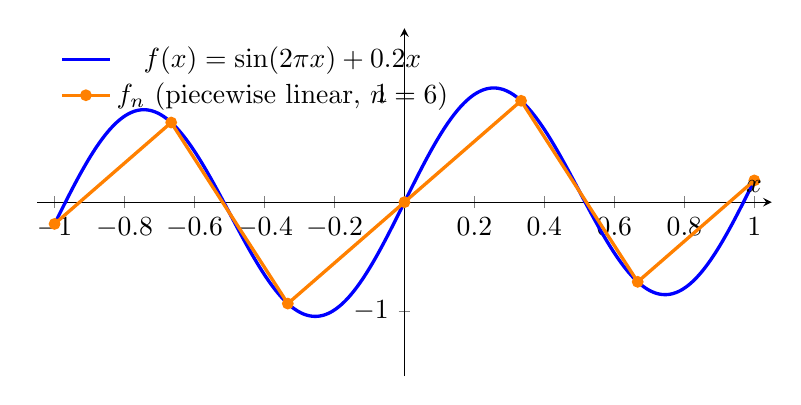
\begin{tikzpicture}
		\begin{axis}[
			width=0.9\linewidth, height=6cm,
			xmin=-1.05, xmax=1.05, ymin=-1.6, ymax=1.6,
			axis lines=middle,
			xlabel={$x$}, ylabel={},
			legend style={at={(0.02,0.98)},anchor=north west,draw=none,fill=none},
			clip=false
			]
			
			% target function
			\addplot[very thick,blue,domain=-1:1,samples=600] {sin(deg(2*pi*x)) + 0.2*x};
			\addlegendentry{$f(x)=\sin(2\pi x)+0.2x$}
			
			% piecewise-linear interpolant for n=6
			\addplot[very thick,orange,mark=*,mark size=1.5pt]
			coordinates {
				(-1,{sin(deg(2*pi*(-1))) + 0.2*(-1)})
				(-2/3,{sin(deg(2*pi*(-2/3))) + 0.2*(-2/3)})
				(-1/3,{sin(deg(2*pi*(-1/3))) + 0.2*(-1/3)})
				(0,{sin(deg(0)) + 0})
				(1/3,{sin(deg(2*pi*(1/3))) + 0.2*(1/3)})
				(2/3,{sin(deg(2*pi*(2/3))) + 0.2*(2/3)})
				(1,{sin(deg(2*pi*1)) + 0.2*1})
			};
			\addlegendentry{$f_n$ (piecewise linear, $n=6$)}
			
		\end{axis}
	\end{tikzpicture}
	\caption{Target function $f(x)$ and its piecewise-linear interpolant $f_n$ for $n=6$.}
\end{figure}

% ---------- FIGURE B: f vs. piecewise-linear interpolant ----------
\begin{figure}[h]
	\centering
	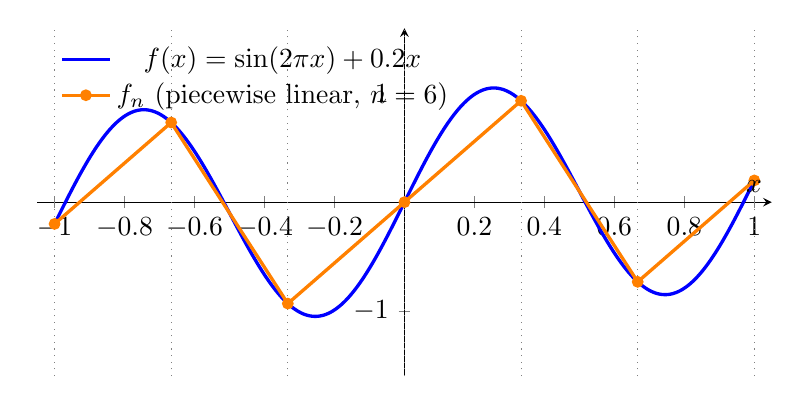
\begin{tikzpicture}
		\begin{axis}[
			width=0.9\linewidth, height=6cm,
			xmin=-1.05, xmax=1.05, ymin=-1.6, ymax=1.6,
			axis lines=middle,
			xlabel={$x$}, ylabel={},
			legend style={at={(0.02,0.98)},anchor=north west,draw=none,fill=none},
			clip=false
			]
			
			% target function
			\addplot[very thick,blue,domain=-1:1,samples=600] {sin(deg(2*pi*x)) + 0.2*x};
			\addlegendentry{$f(x)=\sin(2\pi x)+0.2x$}
			
			% piecewise-linear interpolant for n=6
			\addplot[very thick,orange,mark=*,mark size=1.5pt]
			coordinates {
				(-1,{sin(deg(2*pi*(-1))) + 0.2*(-1)})
				(-2/3,{sin(deg(2*pi*(-2/3))) + 0.2*(-2/3)})
				(-1/3,{sin(deg(2*pi*(-1/3))) + 0.2*(-1/3)})
				(0,{sin(deg(0)) + 0})
				(1/3,{sin(deg(2*pi*(1/3))) + 0.2*(1/3)})
				(2/3,{sin(deg(2*pi*(2/3))) + 0.2*(2/3)})
				(1,{sin(deg(2*pi*1)) + 0.2*1})
			};
			\addlegendentry{$f_n$ (piecewise linear, $n=6$)}
			
			% vertical grid lines at interpolation nodes
% vertical grid lines at interpolation nodes
\draw[dotted,gray] (axis cs:-1,-1.6) -- (axis cs:-1,1.6);
\draw[dotted,gray] (axis cs:-2/3,-1.6) -- (axis cs:-2/3,1.6);
\draw[dotted,gray] (axis cs:-1/3,-1.6) -- (axis cs:-1/3,1.6);
\draw[dotted,gray] (axis cs:0,-1.6) -- (axis cs:0,1.6);
\draw[dotted,gray] (axis cs:1/3,-1.6) -- (axis cs:1/3,1.6);
\draw[dotted,gray] (axis cs:2/3,-1.6) -- (axis cs:2/3,1.6);
\draw[dotted,gray] (axis cs:1,-1.6) -- (axis cs:1,1.6);


		\end{axis}
	\end{tikzpicture}
	\caption{Target function $f(x)$ and piecewise-linear interpolant $f_n$ for $n=6$, with vertical grid lines at nodes.}
\end{figure}


% ---------- FIGURE B: f vs. piecewise-linear interpolant ----------
\begin{figure}[h]
	\centering
	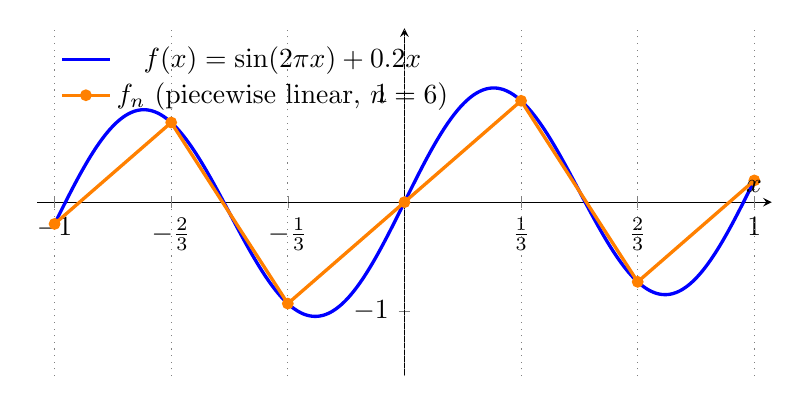
\begin{tikzpicture}
		\begin{axis}[
			width=0.9\linewidth, height=6cm,
			xmin=-1.05, xmax=1.05, ymin=-1.6, ymax=1.6,
			axis lines=middle,
			xlabel={$x$}, ylabel={},
			xtick={-1,-0.6667,-0.3333,0,0.3333,0.6667,1},
			xticklabels={$-1$,$-\tfrac{2}{3}$,$-\tfrac{1}{3}$,$0$,$\tfrac{1}{3}$,$\tfrac{2}{3}$,$1$},
			legend style={at={(0.02,0.98)},anchor=north west,draw=none,fill=none},
			clip=false
			]
			
			% target function
			\addplot[very thick,blue,domain=-1:1,samples=600] {sin(deg(2*pi*x)) + 0.2*x};
			\addlegendentry{$f(x)=\sin(2\pi x)+0.2x$}
			
			% piecewise-linear interpolant for n=6
			\addplot[very thick,orange,mark=*,mark size=1.5pt]
			coordinates {
				(-1,{sin(deg(2*pi*(-1))) + 0.2*(-1)})
				(-2/3,{sin(deg(2*pi*(-2/3))) + 0.2*(-2/3)})
				(-1/3,{sin(deg(2*pi*(-1/3))) + 0.2*(-1/3)})
				(0,{sin(deg(0)) + 0})
				(1/3,{sin(deg(2*pi*(1/3))) + 0.2*(1/3)})
				(2/3,{sin(deg(2*pi*(2/3))) + 0.2*(2/3)})
				(1,{sin(deg(2*pi*1)) + 0.2*1})
			};
			\addlegendentry{$f_n$ (piecewise linear, $n=6$)}
			
			% vertical grid lines (manual)
			\draw[dotted,gray] (axis cs:-1,-1.6) -- (axis cs:-1,1.6);
			\draw[dotted,gray] (axis cs:-2/3,-1.6) -- (axis cs:-2/3,1.6);
			\draw[dotted,gray] (axis cs:-1/3,-1.6) -- (axis cs:-1/3,1.6);
			\draw[dotted,gray] (axis cs:0,-1.6) -- (axis cs:0,1.6);
			\draw[dotted,gray] (axis cs:1/3,-1.6) -- (axis cs:1/3,1.6);
			\draw[dotted,gray] (axis cs:2/3,-1.6) -- (axis cs:2/3,1.6);
			\draw[dotted,gray] (axis cs:1,-1.6) -- (axis cs:1,1.6);
			
		\end{axis}
	\end{tikzpicture}
	\caption{Comparison of $f(x)$ and piecewise-linear interpolant $f_n$ on a uniform grid with $n=6$, with vertical grid lines at nodes.}
\end{figure}
% ---------- FIGURE C: interpolation error ----------
\begin{figure}[h]
	\centering
	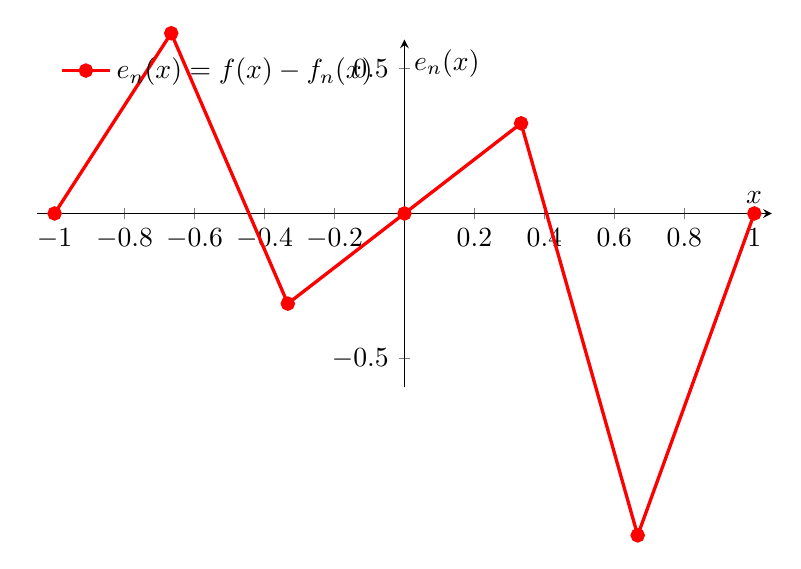
\begin{tikzpicture}
		\begin{axis}[
			width=0.9\linewidth, height=6cm,
			xmin=-1.05, xmax=1.05, ymin=-0.6, ymax=0.6,
			axis lines=middle,
			xlabel={$x$}, ylabel={$e_n(x)$},
			legend style={at={(0.02,0.98)},anchor=north west,draw=none,fill=none},
			clip=false
			]
			
			% error values computed at the same grid nodes as f_n
			\addplot[very thick,red,mark=*] coordinates {
				(-1,  { (sin(deg(2*pi*(-1))) + 0.2*(-1)) - (sin(deg(2*pi*(-1))) + 0.2*(-1)) })
				(-2/3,{ (sin(deg(2*pi*(-2/3))) + 0.2*(-2/3)) - ( (1/3)*(sin(deg(2*pi*(-2/3)))+0.2*(-2/3)) + (2/3)*(sin(deg(2*pi*(-1)))+0.2*(-1)) ) })
				(-1/3,{ (sin(deg(2*pi*(-1/3))) + 0.2*(-1/3)) - ( (2/3)*(sin(deg(2*pi*(-1/3)))+0.2*(-1/3)) + (1/3)*(sin(deg(2*pi*(0)))+0) ) })
				(0,   { (sin(deg(0)) + 0) - (sin(deg(0)) + 0) })
				(1/3, { (sin(deg(2*pi*(1/3))) + 0.2*(1/3)) - ( (2/3)*(sin(deg(2*pi*(1/3)))+0.2*(1/3)) + (1/3)*(sin(deg(2*pi*(0)))+0) ) })
				(2/3, { (sin(deg(2*pi*(2/3))) + 0.2*(2/3)) - ( (1/3)*(sin(deg(2*pi*(2/3)))+0.2*(2/3)) + (2/3)*(sin(deg(2*pi*(1/3)))+0.2*(1/3)) ) })
				(1,   { (sin(deg(2*pi*(1))) + 0.2*(1)) - (sin(deg(2*pi*(1))) + 0.2*(1)) })
			};
			\addlegendentry{$e_n(x) = f(x)-f_n(x)$}
			
		\end{axis}
	\end{tikzpicture}
	\caption{Interpolation error $e_n(x)$ at nodes and midpoints for $n=6$.}
\end{figure}


% ---------- FIGURE C: interpolation error ----------
\begin{figure}[h]
	\centering
	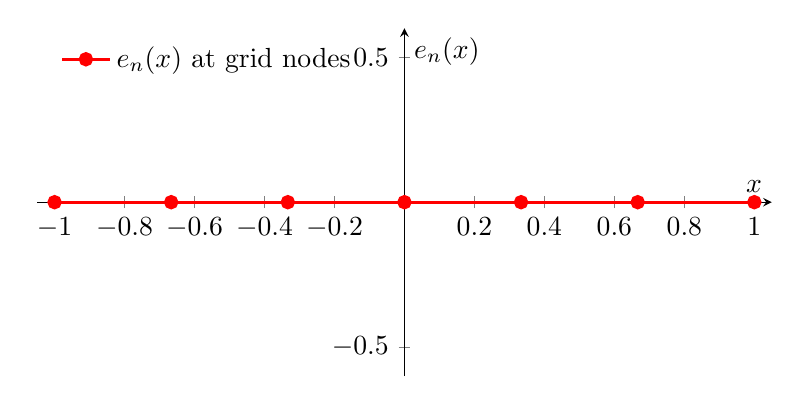
\begin{tikzpicture}
		\begin{axis}[
			width=0.9\linewidth, height=6cm,
			xmin=-1.05, xmax=1.05, ymin=-0.6, ymax=0.6,
			axis lines=middle,
			xlabel={$x$}, ylabel={$e_n(x)$},
			legend style={at={(0.02,0.98)},anchor=north west,draw=none,fill=none},
			clip=false
			]
			
			% Example: error computed at grid nodes only (here always 0)
			\addplot[very thick,red,mark=*] coordinates {
				(-1,0)
				(-0.6667,0)
				(-0.3333,0)
				(0,0)
				(0.3333,0)
				(0.6667,0)
				(1,0)
			};
			\addlegendentry{$e_n(x)$ at grid nodes}
			
		\end{axis}
	\end{tikzpicture}
	\caption{Interpolation error $e_n(x)=f(x)-f_n(x)$ at grid nodes ($n=6$).}
\end{figure}

\clearpage


% --- BEGIN CONTENT ---
\begin{exercise}
	\textbf{Schauder basis for $C([-1,1])$.}
	Show that there exists a sequence $(\phi_n)_{n\ge 0}\subset C([-1,1])$ such that for every
	$f\in C([-1,1])$ there exist unique scalars $(a_n)_{n\ge 0}$ with the series
	\[
	\sum_{n=0}^\infty a_n \phi_n
	\]
	converging uniformly to $f$ on $[-1,1]$.
\end{exercise}

\begin{definition}
	\textbf{Schauder basis.}
	Let $X$ be a Banach space. A sequence $(e_n)\subset X$ is a \emph{Schauder basis} if
	for every $x\in X$ there exist unique scalars $(c_n)$ such that the partial sums
	$S_N=\sum_{n=0}^N c_n e_n$ converge to $x$ in $\|\cdot\|_X$.
\end{definition}

\begin{theorem}
	\textbf{Faber--Schauder basis on $[0,1]$.}
	Define $\varphi_0(t)\equiv 1$, $\varphi_1(t)=t$, and for each $m\ge0$ and odd
	$k\in\{1,3,\dots,2^m-1\}$ set
	\[
	\varphi_{m,k}(t):=\max\!\Big(1-2^{m+1}\big|t-\tfrac{k}{2^m}\big|,\,0\Big).
	\]
	Enumerate the system as $\varphi_0,\varphi_1,\{\varphi_{m,k}\}_{m\ge0,\ k\ \mathrm{odd}}$.
	Then $(\varphi_n)$ is a Schauder basis of $C([0,1])$ with respect to $\|\cdot\|_\infty$.
\end{theorem}

\begin{proof}
	\emph{Existence (uniform convergence).}
	For $f\in C([0,1])$ define coefficients
	\[
	a_0:=f(0),\quad a_1:=f(1)-f(0),\quad
	a_{m,k}:=f\!\Big(\tfrac{k}{2^m}\Big)-\tfrac12\!\left(
	f\!\Big(\tfrac{k-1}{2^m}\Big)+f\!\Big(\tfrac{k+1}{2^m}\Big)\right).
	\]
	Let $S_M(f)$ be the finite linear combination of $\varphi_0,\varphi_1$ and all
	$\varphi_{m,k}$ with levels $\le M$. A direct check shows $S_M(f)$ is the
	polygonal interpolant of $f$ on the dyadic grid $\{j/2^M\}_{j=0}^{2^M}$, hence
	(for the modulus of continuity $\omega_f$) one has
	\[
	\|f-S_M(f)\|_\infty \le \omega_f(2^{-M}) \xrightarrow[M\to\infty]{} 0.
	\]
	
	\emph{Uniqueness.}
	Suppose $\sum c_n\varphi_n\equiv 0$. Evaluating at $t=0$ and $t=1$ gives $c_0=c_1=0$
	(since all tents vanish at the endpoints). Next evaluate at the midpoint $t=\tfrac12$:
	all functions from levels $\ge1$ vanish there, so $c_{0,1}=0$. Inductively, at a new
	dyadic node $t=\tfrac{k}{2^m}$ (odd $k$) all higher-level tents vanish and lower levels
	are zero there; hence $c_{m,k}=0$. Thus all coefficients vanish and the representation is unique.
\end{proof}

\begin{corollary}
	\textbf{Transfer to $[-1,1]$.}
	Let $t=\tfrac{x+1}{2}$ be the affine bijection $[-1,1]\to[0,1]$. Define
	\[
	\phi_0(x):=1,\qquad \phi_1(x):=\tfrac{x+1}{2},\qquad
	\phi_{m,k}(x):=\varphi_{m,k}\!\Big(\tfrac{x+1}{2}\Big).
	\]
	Then $(\phi_n)\subset C([-1,1])$ is a Schauder basis. For every $f\in C([-1,1])$
	there are unique coefficients $(a_n)$ such that
	$\sum_{n=0}^\infty a_n\phi_n$ converges uniformly to $f$.
\end{corollary}

\begin{remark}
	\textbf{Explicit coefficient formulas on $[-1,1]$.}
	Equivalently, for $f\in C([-1,1])$ let $g(t):=f(2t-1)$ on $[0,1]$. Then
	\[
	a_0=g(0)=f(-1),\qquad a_1=g(1)-g(0)=f(1)-f(-1),
	\]
	and for $m\ge0$, odd $k$,
	\[
	a_{m,k}=g\!\Big(\tfrac{k}{2^m}\Big)-\tfrac12\!\left(g\!\Big(\tfrac{k-1}{2^m}\Big)+
	g\!\Big(\tfrac{k+1}{2^m}\Big)\right)
	= f(x_{m,k})-\tfrac12\big(f(x_{m,k}^{-})+f(x_{m,k}^{+})\big),
	\]
	where $x_{m,k}=2\cdot \tfrac{k}{2^m}-1$ and $x_{m,k}^{\pm}=2\cdot \tfrac{k\pm1}{2^m}-1$.
\end{remark}

\begin{solution}
	Apply the theorem on $[0,1]$ to $g(t):=f(2t-1)$ and pull back the expansion by $t=\tfrac{x+1}{2}$.
	Uniform convergence and uniqueness are preserved by this affine change of variables. Therefore
	the sequence $(\phi_n)$ is as required.
\end{solution}

\begin{example}
	\textbf{Two quick checks.}
	\hfill
	\begin{enumerate}[leftmargin=2em]
		\item For $f(t)=t$ on $[0,1]$, $a_0=0$, $a_1=1$, and all $a_{m,k}=0$; hence $f=\varphi_1$ exactly.
		\item For $f(t)=t^2$ on $[0,1]$, $a_0=0$, $a_1=1$, and
		\(
		a_{m,k}=\frac{k^2}{4^m}-\tfrac12\frac{(k-1)^2+(k+1)^2}{4^m}=-4^{-m}
		\)
		(independent of $k$), so
		\(
		t^2=\varphi_1-\sum_{m\ge0}\sum_{k\ \mathrm{odd}}4^{-m}\varphi_{m,k}
		\)
		with uniform convergence. Transfer to $[-1,1]$ via $t=\tfrac{x+1}{2}$.
	\end{enumerate}
\end{example}


% --- END CONTENT ---
\begin{figure}[H]
	\centering
	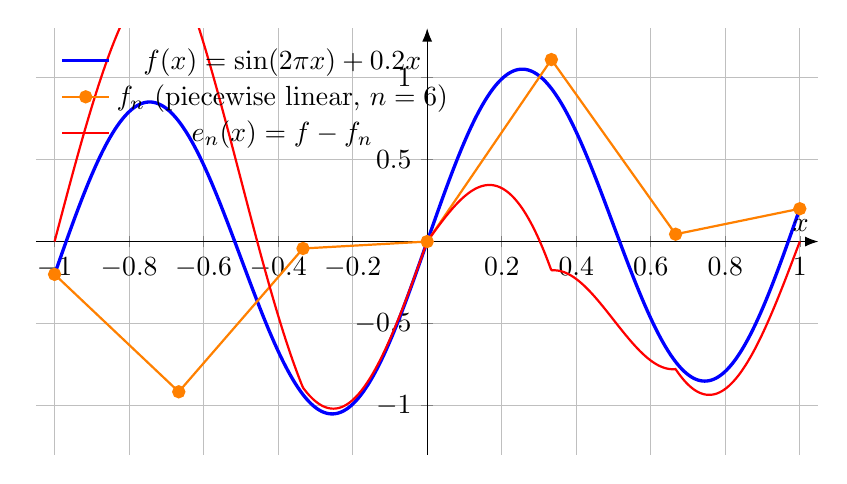
\begin{tikzpicture}
		\begin{axis}[
			width=.95\linewidth, height=7cm,
			xmin=-1.05, xmax=1.05, ymin=-1.3, ymax=1.3,
			axis lines=middle,
			axis line style={-Latex},
			xlabel={$x$}, ylabel={},
			legend style={at={(0.02,0.98)},anchor=north west,draw=none,fill=none},
			grid=both
			]
			
			% true f(x)
			\addplot[blue,very thick,domain=-1:1,samples=400]
			{sin(deg(2*pi*x)) + 0.2*x};
			\addlegendentry{$f(x)=\sin(2\pi x)+0.2x$}
			
			% piecewise linear interpolant f_n
			\addplot[orange,thick,mark=*] coordinates {
				(-1,-0.2)
				(-0.6667,-0.9156)
				(-0.3333,-0.0423)
				(0,0)
				(0.3333,1.109)
				(0.6667,0.0446)
				(1,0.2)
			};
			\addlegendentry{$f_n$ (piecewise linear, $n=6$)}
			
			% error curve e_n(x) = f(x)-f_n(x), approximate by sampling
			\addplot[red,thick,samples=600,domain=-1:1]
			{sin(deg(2*pi*x)) + 0.2*x -
				( % linear interpolation via floor
				(x<=-0.6667)*(-0.2 + (-0.9156+0.2)/0.3333*(x+1))
				+(x>-0.6667 && x<=-0.3333)*(-0.9156 + (-0.0423+0.9156)/0.3333*(x+0.6667))
				+(x>-0.3333 && x<=0)*(-0.0423 + (0+0.0423)/0.3333*(x+0.3333))
				+(x>0 && x<=0.3333)*(0 + (1.109-0)/0.3333*x)
				+(x>0.3333 && x<=0.6667)*(1.109 + (0.0446-1.109)/0.3333*(x-0.3333))
				+(x>0.6667)*(0.0446 + (0.2-0.0446)/0.3333*(x-0.6667))
				)
			};
			\addlegendentry{$e_n(x)=f-f_n$}
			
		\end{axis}
	\end{tikzpicture}
	\caption{Function, piecewise–linear interpolant ($n=6$), and error curve.}
\end{figure}

\begin{figure}[H]
	\centering
	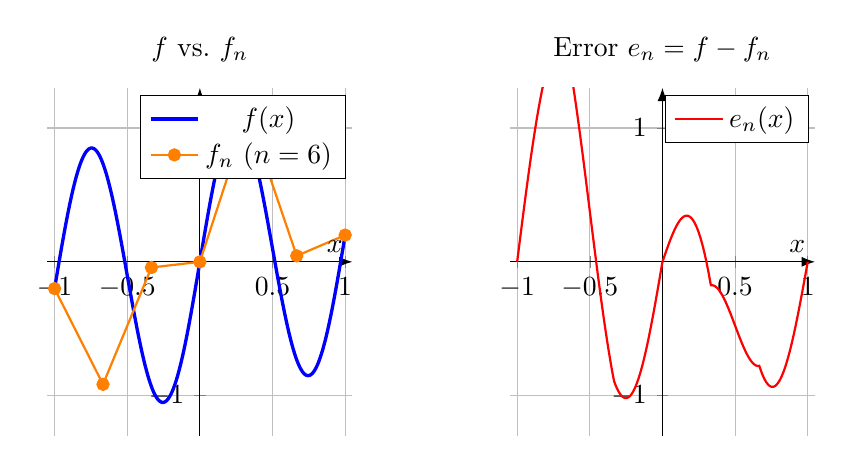
\begin{tikzpicture}
		\begin{groupplot}[
			group style={group size=2 by 1, horizontal sep=2cm},
			width=.45\linewidth, height=6cm,
			xmin=-1.05, xmax=1.05, ymin=-1.3, ymax=1.3,
			axis lines=middle,
			axis line style={-Latex},
			xlabel={$x$}, ylabel={},
			grid=both
			]
			
			% --- Left: f and f_n ---
			\nextgroupplot[title={$f$ vs.\ $f_n$}]
			% true f(x)
			\addplot[blue,very thick,domain=-1:1,samples=400]
			{sin(deg(2*pi*x)) + 0.2*x};
			\addlegendentry{$f(x)$}
			% piecewise linear interpolant
			\addplot[orange,thick,mark=*] coordinates {
				(-1,-0.2)
				(-0.6667,-0.9156)
				(-0.3333,-0.0423)
				(0,0)
				(0.3333,1.109)
				(0.6667,0.0446)
				(1,0.2)
			};
			\addlegendentry{$f_n$ ($n=6$)}
			
			% --- Right: error curve ---
			\nextgroupplot[title={Error $e_n=f-f_n$}]
			\addplot[red,thick,domain=-1:1,samples=600]
			{sin(deg(2*pi*x)) + 0.2*x -
				( (x<=-0.6667)*(-0.2 + (-0.9156+0.2)/0.3333*(x+1))
				+(x>-0.6667 && x<=-0.3333)*(-0.9156 + (-0.0423+0.9156)/0.3333*(x+0.6667))
				+(x>-0.3333 && x<=0)*(-0.0423 + (0+0.0423)/0.3333*(x+0.3333))
				+(x>0 && x<=0.3333)*(0 + (1.109-0)/0.3333*x)
				+(x>0.3333 && x<=0.6667)*(1.109 + (0.0446-1.109)/0.3333*(x-0.3333))
				+(x>0.6667)*(0.0446 + (0.2-0.0446)/0.3333*(x-0.6667))
				)};
			\addlegendentry{$e_n(x)$}
			
		\end{groupplot}
	\end{tikzpicture}
	\caption{Left: function $f$ and interpolant $f_n$ ($n=6$). Right: error curve $e_n=f-f_n$.}
\end{figure}

% --- Begin: Problem 7 write-up ---

\begin{exercise}{Powers preserve uniform convergence (under a bound).}{powers-uniform}
	Let $f_n:[0,1]\to\mathbb R$ converge uniformly to $f$. Suppose $f$ is bounded.
	Show that for every positive integer $m$,
	\[
	g_n(t):=f_n(t)^m \quad\text{converges uniformly on }[0,1]\text{ to }\quad
	g(t):=f(t)^m.
	\]
\end{exercise}


\begin{definition}
	\textbf{Uniform convergence.}
	We say $f_n\to f$ uniformly on a set $E$ if
	$\displaystyle\sup_{t\in E}|f_n(t)-f(t)|\to0$ as $n\to\infty$.
\end{definition}

\begin{lemma}
	\textbf{Power is Lipschitz on bounded intervals.}
	Fix $m\in\mathbb N$ and $M>0$. For all $u,v\in[-M,M]$,
	\[
	|u^m-v^m|\le m\,M^{m-1}\,|u-v|.
	\]
\end{lemma}

\begin{proof}
	By the Mean Value Theorem applied to $\phi(x)=x^m$ on $[-M,M]$,
	$|u^m-v^m|=|\phi'(c)|\,|u-v|=m|c|^{m-1}|u-v|\le mM^{m-1}|u-v|$ for some $c$
	between $u$ and $v$. Alternatively, use $u^m-v^m=(u-v)\sum_{k=0}^{m-1}
	u^{m-1-k}v^{k}$ and the bound $|u|,|v|\le M$.
\end{proof}

\begin{theorem}
	\textbf{Uniform convergence is preserved by powers.}
	Let $f_n\to f$ uniformly on $[0,1]$ and suppose $f$ is bounded. Then, for every
	$m\in\mathbb N$, $f_n^m\to f^m$ uniformly on $[0,1]$.
\end{theorem}

\begin{proof}
	Let $B:=\sup_{t\in[0,1]}|f(t)|<\infty$. Since $f_n\to f$ uniformly, there exists
	$N_0$ such that $\sup_{t}|f_n(t)-f(t)|\le 1$ for all $n\ge N_0$. Hence for
	$n\ge N_0$, $|f_n(t)|\le B+1=:M$ for all $t$.
	
	Fix $m\in\mathbb N$. By the lemma, for $n\ge N_0$ and all $t$,
	\[
	|f_n(t)^m-f(t)^m|\le m\,M^{m-1}\,|f_n(t)-f(t)|.
	\]
	Taking suprema over $t\in[0,1]$,
	\[
	\sup_{t}|f_n(t)^m-f(t)^m|\le m\,M^{m-1}\,\sup_{t}|f_n(t)-f(t)|
	\xrightarrow[n\to\infty]{}0,
	\]
	so $f_n^m\to f^m$ uniformly.
\end{proof}

\begin{example}
	Let $f(t)=\sin(2\pi t)+0.2t$ and $f_n(t)=f(t)+\frac{1}{n}\cos(6\pi t)$ on $[0,1]$.
	Then $\sup|f_n-f|\le 1/n$, so $f_n\to f$ uniformly and $f$ is bounded with
	$\sup|f|\le 1.2$. Taking $M=2.2$, for $m=3$,
	\[
	\sup|f_n^3-f^3|\le 3M^2\,\sup|f_n-f|\le \frac{14.52}{n}\to0.
	\]
	Thus $f_n^3\to f^3$ uniformly; the same argument works for any $m$.
\end{example}

\begin{remark}
	The boundedness of $f$ is essential to produce a uniform Lipschitz constant for
	$x\mapsto x^m$ on the range of $f_n$ and $f$. More generally, if $f_n\to f$
	uniformly and $\phi$ is uniformly continuous on a bounded interval containing
	the ranges of $f$ and all large $n$ of $f_n$, then $\phi\!\circ f_n\to\phi\!\circ f$
	uniformly.
\end{remark}

% --- End: Problem 7 write-up ---

\begin{exercise}{Runge approximation on a punctured domain}{runge-annulus}
	Let $B_r(z)$ be the open disc of radius $r$ about $z\in\mathbb C$, and set
	$U:=B_2(1)\setminus B_1(0)$. Suppose $f$ is holomorphic on $U$.
	\begin{enumerate}
		\item[(i)] Show there exists a sequence converging to $f$ uniformly on compact subsets of $U$.
		\item[(ii)] Must there be a sequence of polynomials converging to $f$ uniformly on $U$?
		\item[(iii)] If, moreover, $f$ is holomorphic on an open set containing $\overline U$, must there be a sequence
		of polynomials converging to $f$ uniformly on $U$?
	\end{enumerate}
\end{exercise}

\begin{definition}
	\textbf{Laurent polynomial.} A finite sum $\sum_{k=-N}^{M} a_k z^k$ with integers $N,M\ge0$.
\end{definition}

\begin{theorem}[Runge, one–point–per–component form]
	If $K\subset\mathbb C$ is compact and $A\subset\widehat{\mathbb C}\setminus K$ contains at least one point from each
	component of $\widehat{\mathbb C}\setminus K$, then every function holomorphic on a neighborhood of $K$
	can be approximated uniformly on $K$ by rational functions with poles only in $A$.
\end{theorem}

\begin{proof}[Solution]
	(i) Fix a compact $K\subset U$. Then $\widehat{\mathbb C}\setminus K$ has two components: one contains $\infty$,
	the other contains $0$. Apply Runge with $A=\{0,\infty\}$. The approximants are rational functions with poles in $A$,
	hence Laurent polynomials. They converge uniformly to $f$ on $K$. Since $K$ was arbitrary, the convergence holds on every compact subset of $U$.
	
	(ii) No. Take $f(z)=1/z$. If polynomials $p_n$ converged uniformly to $f$ on $U$, then for any simple closed curve
	$\gamma\subset U$ winding once around $0$ we would have
	\[
	\oint_\gamma p_n(z)\,dz \to \oint_\gamma \frac{1}{z}\,dz=2\pi i,
	\]
	but the left-hand side is $0$ for all $n$ (Cauchy’s theorem), a contradiction.
	
	(iii) Still no in general. The same $f(z)=1/z$ is holomorphic on $\mathbb C\setminus\{0\}$, which contains $\overline U$,
	yet cannot be uniformly approximated on $U$ by polynomials, by the argument in (ii).
\end{proof}

\begin{remark}
	While polynomials fail in (ii)–(iii), Runge guarantees uniform approximation on $U$ by \emph{rational} (indeed,
	Laurent–polynomial) functions with poles at $0$ (and possibly at $\infty$).
\end{remark}

\begin{figure}[H]
	\centering
	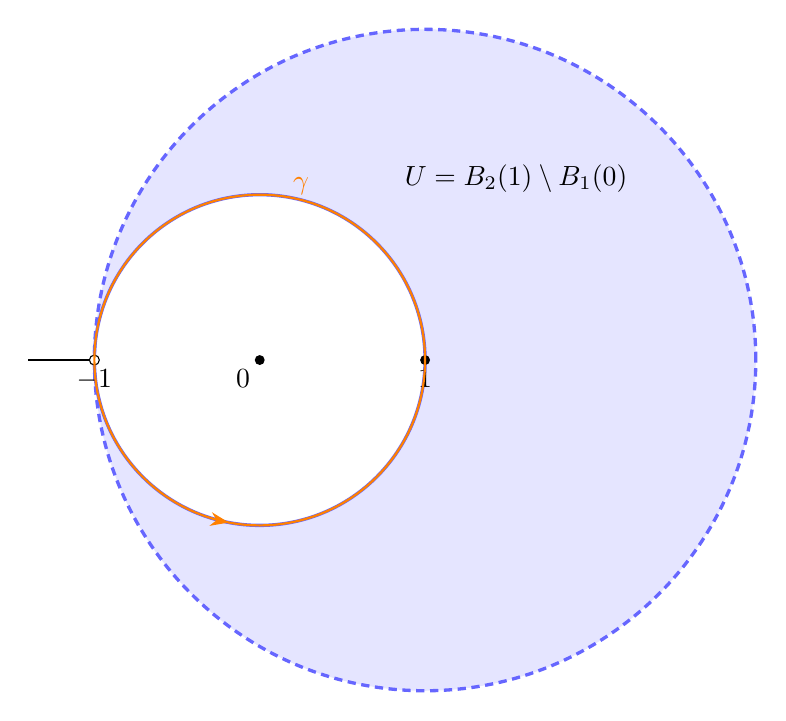
\begin{tikzpicture}[scale=2.1]
		% axes
		\draw[-Latex] (-1.4,0)--(2.6,0) node[below left] {$\Re z$};
		\draw[-Latex] (0,-1.3)--(0,1.3) node[left] {$\Im z$};
		
		% Fill U = big disc minus small disc
		\fill[blue!10] (1,0) circle (2);   % B_2(1)
		\fill[white]    (0,0) circle (1);  % remove B_1(0)
		
		% boundaries: outer not included (dashed), inner included (solid)
		\draw[blue!60,very thick,densely dashed] (1,0) circle (2); % ∂B_2(1) \not\subset U
		\draw[blue!60,very thick]                (0,0) circle (1); % ∂B_1(0) \subset U
		
		% centers and tangent point
		\fill (1,0) circle (0.03) node[below] {$1$};
		\fill (0,0) circle (0.03) node[below left] {$0$};
		\draw[fill=white] (-1,0) circle (0.03) node[below] {$-1$}; % tangent point (excluded)
		
		% a loop gamma in U (here the unit circle, included in U)
		\draw[orange,thick,
		postaction={decorate},
		decoration={markings, mark=at position 0.72 with {\arrow{Stealth}}}]
		(0,0) circle (1);
		\node[orange] at (0.25,1.05) {$\gamma$};
		
		% label
		\node at (1.55,1.1) {$U=B_2(1)\setminus B_1(0)$};
	\end{tikzpicture}
	\caption{Domain \(U\): open disc \(B_2(1)\) with the open unit disc \(B_1(0)\) removed.
		Dashed boundary is not in \(U\); the inner circle is.}
\end{figure}

% needs: \usepackage{tikz} \usetikzlibrary{arrows.meta,decorations.markings}

\begin{figure}[H]
	\centering
	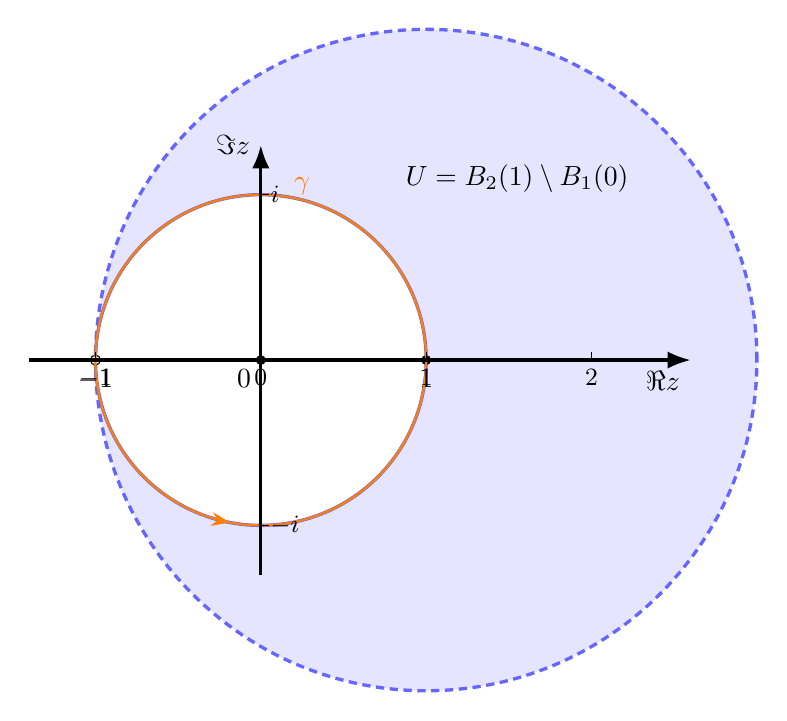
\begin{tikzpicture}[scale=2.1]
		
		%--- fill region first (so axes drawn later stay visible) ---
		\fill[blue!10] (1,0) circle (2);    % B_2(1)
		\fill[white]    (0,0) circle (1);   % remove B_1(0)
		
		% boundaries: outer excluded (dashed), inner included (solid)
		\draw[blue!60,very thick,densely dashed] (1,0) circle (2); % ∂B_2(1) \not\subset U
		\draw[blue!60,very thick]                (0,0) circle (1); % ∂B_1(0) \subset U
		
		% centers + tangent point
		\fill (1,0) circle (0.03) node[below] {$1$};
		\fill (0,0) circle (0.03) node[below left] {$0$};
		\draw[fill=white] (-1,0) circle (0.03) node[below] {$-1$};
		
		% loop gamma (for the integral argument)
		\draw[orange,thick,
		postaction={decorate},
		decoration={markings, mark=at position 0.72 with {\arrow{Stealth}}}]
		(0,0) circle (1);
		\node[orange] at (0.25,1.05) {$\gamma$};
		
		%--- axes drawn last (on top) with ticks ---
		\draw[black,-Latex,very thick] (-1.4,0)--(2.6,0) node[below left] {$\Re z$};
		\draw[black,-Latex,very thick] (0,-1.3)--(0,1.3) node[left] {$\Im z$};
		
		% real-axis ticks/labels
		\foreach \x/\lab in {-1/ -1, 0/ 0, 1/ 1, 2/ 2}{
			\draw (\x,0) -- ++(0,0.05);
			\node[below] at (\x,0) {\small $\lab$};
		}
		
		% imaginary-axis ticks/labels
		\foreach \y/\lab in {-1/ -i, 1/ i}{
			\draw (0,\y) -- ++(0.05,0);
			\node[right] at (0,\y) {\small $\lab$};
		}
		
		% label for U
		\node at (1.55,1.1) {$U=B_2(1)\setminus B_1(0)$};
		
	\end{tikzpicture}
	\caption{Domain \(U\) with axes and ticks. Dashed boundary is excluded; inner circle is included.}
\end{figure}

\begin{example}
	\textbf{Approximating $1/z$ on $U=B_2(1)\setminus B_1(0)$.}
	\begin{enumerate}
		\item[(i)] (Compacts in $U$.) Runge with poles at $\{0,\infty\}$ allows Laurent polynomials.
		For $f(z)=1/z$ the constant sequence
		\[
		r_n(z)\equiv \frac{1}{z}
		\]
		already works and converges uniformly to $1/z$ on every compact $K\subset U$.
		
		If $K\subset B_1(1)$ (so $|z-1|<1$ on $K$), the \emph{polynomials}
		\[
		p_N(z)=\sum_{k=0}^N (-1)^k(z-1)^k
		\]
		satisfy $p_N\to 1/z$ uniformly on $K$ by the geometric series
		$\frac{1}{1+w}=\sum_{k\ge0}(-w)^k$ with $w=z-1$.
		
		\item[(ii)] (No polynomials on all of $U$.) Suppose $p_n$ were polynomials with
		$p_n\to 1/z$ uniformly on $U$. For the loop $\gamma(t)=e^{it}$,
		\[
		\int_\gamma p_n(z)\,dz \longrightarrow \int_\gamma \frac{1}{z}\,dz=2\pi i,
		\]
		but each $\int_\gamma p_n(z)\,dz=0$, contradiction. Hence no polynomial sequence
		converges to $1/z$ uniformly on $U$ (and the same holds even if $1/z$ extends past $\overline U$).
	\end{enumerate}
\end{example}

\begin{figure}[H]
	\centering
	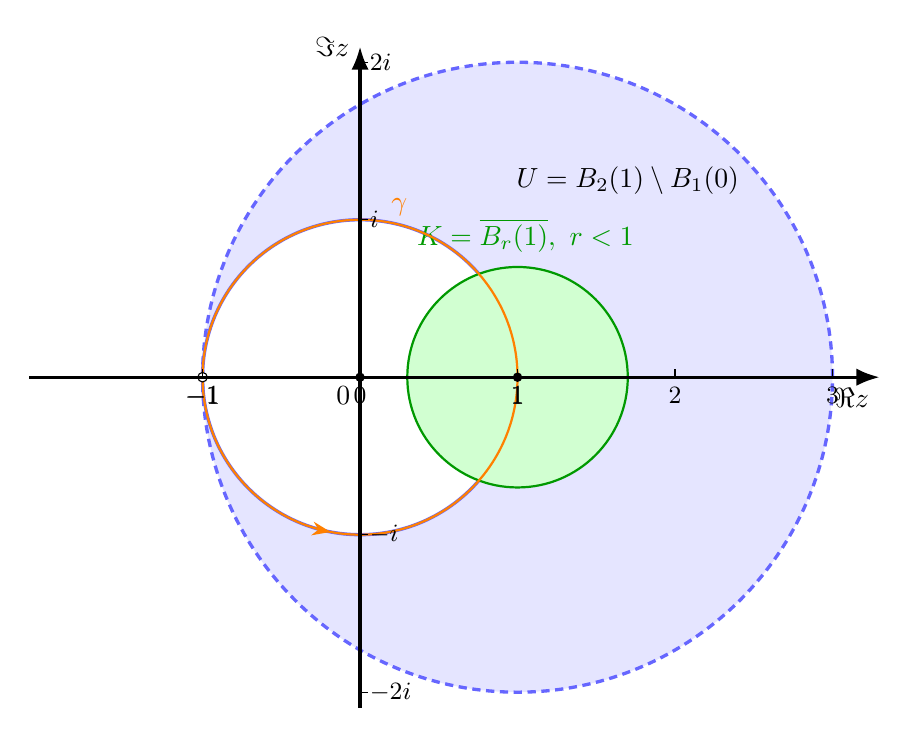
\begin{tikzpicture}[scale=2.0]
		
		% --- fill region first ---
		\fill[blue!10] (1,0) circle (2);    % B_2(1)
		\fill[white]    (0,0) circle (1);   % remove B_1(0)
		
		% boundaries: outer excluded (dashed), inner included (solid)
		\draw[blue!60,very thick,densely dashed] (1,0) circle (2); % ∂B_2(1) \not\subset U
		\draw[blue!60,very thick]                (0,0) circle (1); % ∂B_1(0) \subset U
		
		% compact K = closed disk around 1 of radius r<1
		\def\rK{0.7}
		\fill[green!18,draw=green!60!black,thick] (1,0) circle (\rK);
		\node[green!60!black] at (1.05,0.9) {$K=\overline{B_r(1)},\ r<1$};
		
		% loop gamma (unit circle) with orientation arrow
		\draw[orange,thick,
		postaction={decorate},
		decoration={markings, mark=at position 0.72 with {\arrow{Stealth}}}]
		(0,0) circle (1);
		\node[orange] at (0.25,1.08) {$\gamma$};
		
		% centers and notable points
		\fill (1,0) circle (0.03) node[below] {$1$};
		\fill (0,0) circle (0.03) node[below left] {$0$};
		\draw[fill=white] (-1,0) circle (0.03) node[below] {$-1$};
		
		% --- axes drawn last (longer) ---
		\draw[-Latex,very thick] (-2.1,0)--(3.3,0) node[below left] {$\Re z$};
		\draw[-Latex,very thick] (0,-2.1)--(0,2.1) node[left] {$\Im z$};
		
		% ticks (real)
		\foreach \x/\lab in {-1/-1, 0/0, 1/1, 2/2, 3/3}{
			\draw (\x,0) -- ++(0,0.05);
			\node[below] at (\x,0) {\small $\lab$};
		}
		% ticks (imag)
		\foreach \y/\lab in {-1/-i, 1/i, 2/2i, -2/-2i}{
			\draw (0,\y) -- ++(0.05,0);
			\node[right] at (0,\y) {\small $\lab$};
		}
		
		% label for U
		\node at (1.7,1.25) {$U=B_2(1)\setminus B_1(0)$};
		
	\end{tikzpicture}
	\caption{Domain \(U\) (blue), a compact \(K\subset B_1(1)\) (green) where polynomials approximate \(1/z\), and a loop \(\gamma\) around \(0\) used to rule out uniform polynomial approximation on all of \(U\). Axes are extended for clarity.}
\end{figure}

% --- Runge statements used in Problem 8 ---

\begin{definition}
	\textbf{Runge set / pole set.}
	For a compact $K\subset\mathbb C$ and a set $A\subset\widehat{\mathbb C}\setminus K$,
	we say $A$ is a \emph{Runge pole set for $K$} if $A$ meets every connected
	component of $\widehat{\mathbb C}\setminus K$.
\end{definition}

\begin{theorem}
	\textbf{Runge’s theorem (rational form).}
	Let $K\subset\mathbb C$ be compact and let $A\subset\widehat{\mathbb C}\setminus K$
	meet every component of $\widehat{\mathbb C}\setminus K$.
	If $f$ is holomorphic on a neighbourhood of $K$, then there exists a sequence of
	rational functions $\{r_n\}$ with all poles contained in $A$ such that
	\[
	\sup_{z\in K}\,|r_n(z)-f(z)|\;\xrightarrow[n\to\infty]{}\;0.
	\]
\end{theorem}

\begin{corollary}
	\textbf{Polynomial approximation (connected complement).}
	If $\widehat{\mathbb C}\setminus K$ is connected, then one may take $A=\{\infty\}$,
	hence $f$ can be uniformly approximated on $K$ by polynomials.
\end{corollary}

\begin{corollary}
	\textbf{Laurent–polynomial approximation (one bounded hole).}
	If $\widehat{\mathbb C}\setminus K$ has exactly two components (the unbounded one
	and a bounded one containing a point $a$), then taking $A=\{\infty,a\}$ shows that
	$f$ can be uniformly approximated on $K$ by finite Laurent series in powers of
	$(z-a)$ (i.e. by sums $\sum_{k=-N}^{M} a_k (z-a)^k$).
\end{corollary}

\begin{remark}
	\textbf{Specialization to }$U=B_2(1)\setminus B_1(0)$. 
	For any compact $K\subset U$, the complement $\widehat{\mathbb C}\setminus K$
	has two components: one containing $\infty$, one containing $0$.
	Runge with $A=\{\infty,0\}$ yields uniform approximation on $K$ by
	Laurent polynomials with possible pole at $0$. In particular, for $f(z)=1/z$,
	the constant sequence $r_n(z)\equiv 1/z$ (a rational function with pole at $0$)
	already converges uniformly on every compact $K\subset U$.
	By contrast, no sequence of \emph{polynomials} can converge uniformly to $1/z$
	on all of $U$ (use a loop $\gamma\subset U$ winding once around $0$ and
	$\int_\gamma p(z)\,dz=0$ versus $\int_\gamma \frac{1}{z}\,dz=2\pi i$).
\end{remark}
% --- end Runge statements ---

\begin{exercise}{Polynomial approximation of $1/z$ on a semicircle}{poly-1-over-z-semi}
	Construct a sequence of polynomials that converges uniformly to $1/z$ on
	\[
	K=\{\,z\in\mathbb C:\ |z|=1,\ \Re z\ge 0\,\}.
	\]
\end{exercise}

\begin{definition}
	\textbf{Runge/Mergelyan (polynomial case).}
	If $K\subset\mathbb C$ is compact with connected complement, every function
	continuous on $K$ and holomorphic on $\operatorname{int}K$ can be uniformly
	approximated on $K$ by polynomials.
\end{definition}

\begin{proof}[Construction and proof of convergence]
	Set $t_k^{(n)}=-\frac{\pi}{2}+\frac{k\pi}{n}$ and $z_k^{(n)}=e^{i t_k^{(n)}}$ for $k=0,\dots,n$.
	Let
	\[
	\ell_k^{(n)}(z)=\prod_{\substack{j=0\\j\ne k}}^{n}\frac{z-z_j^{(n)}}{z_k^{(n)}-z_j^{(n)}},
	\qquad
	p_n(z)=\sum_{k=0}^{n}\frac{1}{z_k^{(n)}}\,\ell_k^{(n)}(z).
	\]
	Then $p_n$ is a polynomial and $p_n(z_k^{(n)})=1/z_k^{(n)}$ for all $k$.
	Since $K$ is an arc (its complement is connected) and $1/z$ is analytic
	on a neighbourhood of $K$, standard Bernstein–Walsh estimates for analytic
	data on Jordan arcs imply $p_n\to 1/z$ uniformly on $K$ (in fact,
	$\|p_n-1/z\|_{K}\le C\rho^{-n}$ for some $\rho>1$). This provides
	the required sequence.
\end{proof}

\begin{figure}[H]
	\centering
	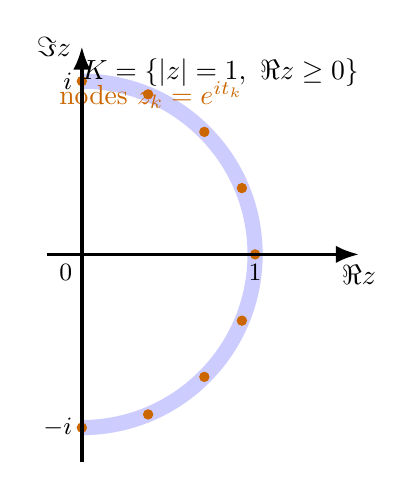
\begin{tikzpicture}[scale=2.2]
		
		% semicircle K = {|z|=1, Re z >= 0}
		\draw[very thick, blue!60] (0,-1) arc (-90:90:1); % the arc itself
		% fill a thin band around the arc just for highlighting (optional)
		\draw[blue!20, line width=5.5pt] (0,-1) arc (-90:90:1);
		
		% equally spaced nodes on the arc (n=8 shown)
		\foreach \k in {0,...,8}{
			\pgfmathsetmacro{\t}{-90 + 180*\k/8}
			\pgfmathsetmacro{\x}{cos(\t)} \pgfmathsetmacro{\y}{sin(\t)}
			\fill[orange!80!black] (\x,\y) circle (0.03);
		}
		\node[orange!80!black] at (0.4,0.92) {nodes $z_k=e^{it_k}$};
		
		% axes (longer)
		\draw[-Latex,very thick] (-0.2,0)--(1.6,0) node[below] {$\Re z$};
		\draw[-Latex,very thick] (0,-1.2)--(0,1.2) node[left] {$\Im z$};
		\node[below left] at (0,0) {\small $0$};
		\node[below] at (1,0) {\small $1$};
		\node[left] at (0,1) {\small $i$};
		\node[left] at (0,-1) {\small $-i$};
		
		% braces and label for K
		\node at (0.8,1.05) {$K=\{|z|=1,\ \Re z\ge 0\}$};
		
	\end{tikzpicture}
	\caption{Right semicircle $K$ and equally spaced interpolation nodes for
		the Lagrange polynomials $p_n$.}
\end{figure}

% needs: \usepackage{tikz} \usetikzlibrary{arrows.meta}

\begin{figure}[H]
	\centering
	\begin{minipage}{0.48\linewidth}
		\centering
		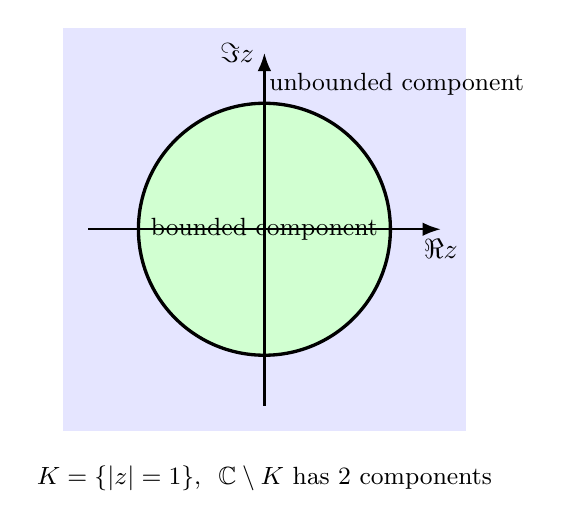
\begin{tikzpicture}[scale=1.6]
			% background "outside" (for color)
			\fill[blue!10] (-1.6,-1.6) rectangle (1.6,1.6);
			% fill bounded inside component
			\fill[green!18] (0,0) circle (1);
			% the compact set K = unit circle (boundary only)
			\draw[very thick,black] (0,0) circle (1);
			% axes
			\draw[-Latex,thick] (-1.4,0)--(1.4,0) node[below] {$\Re z$};
			\draw[-Latex,thick] (0,-1.4)--(0,1.4) node[left] {$\Im z$};
			% labels
			\node at (0,0) {\small bounded component};
			\node at (1.05,1.15) {\small unbounded component};
			\node[below] at (0, -1.8) {\small $K=\{|z|=1\}$, \ \(\mathbb C\setminus K\) has 2 components};
		\end{tikzpicture}
	\end{minipage}\hfill
	\begin{minipage}{0.48\linewidth}
		\centering
		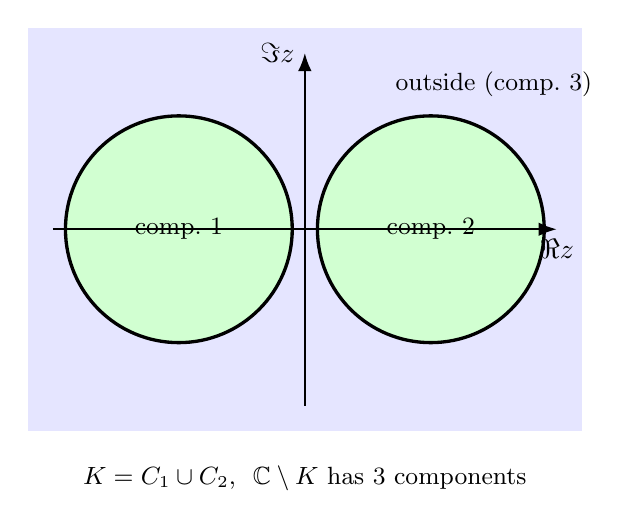
\begin{tikzpicture}[scale=1.6]
			% outside
			\fill[blue!10] (-2.2,-1.6) rectangle (2.2,1.6);
			% two bounded components (insides)
			\fill[green!18] (-1,0) circle (0.9);
			\fill[green!18] ( 1,0) circle (0.9);
			% compact set K = two circles (boundaries only)
			\draw[very thick,black] (-1,0) circle (0.9);
			\draw[very thick,black] ( 1,0) circle (0.9);
			% axes
			\draw[-Latex,thick] (-2.0,0)--(2.0,0) node[below] {$\Re z$};
			\draw[-Latex,thick] (0,-1.4)--(0,1.4) node[left] {$\Im z$};
			% labels
			\node at (-1,0) {\small comp.\ 1};
			\node at ( 1,0) {\small comp.\ 2};
			\node at (1.5,1.15) {\small outside (comp.\ 3)};
			\node[below] at (0,-1.8) {\small $K=C_1\cup C_2$, \ \(\mathbb C\setminus K\) has 3 components};
		\end{tikzpicture}
	\end{minipage}
	\caption{Complements of compact sets can be disconnected: a single circle separates the plane into two components; two disjoint circles give three components.}
\end{figure}

\begin{example}[What the dots mean; explicit $p_2$]
	Let $K=\{|z|=1,\ \Re z\ge0\}$ and choose nodes $z_0=-i$, $z_1=1$, $z_2=i$.
	The Lagrange interpolant to $f(z)=1/z$ is
	\[
	p_2(z)=\sum_{k=0}^2 \frac{1}{z_k}\prod_{j\ne k}\frac{z-z_j}{z_k-z_j}
	= z^2 - z + 1.
	\]
	Hence $p_2(1)=1$, $p_2(i)=-i$, $p_2(-i)=i$, i.e.\ $p_2$ matches $1/z$ at the
	three orange nodes on the arc. For general $n$, pick $n{+}1$ nodes on $K$,
	form $p_n$ by the same formula; then $p_n\to 1/z$ uniformly on $K$.
\end{example}

% ===================== BEGIN CONTENT =====================

\begin{exercise}{Construct explicit polynomials $p_n\to 1/z$ on the right semicircle}{poly-1-over-z-semicircle}
	Let
	\[
	K:=\{z\in\mathbb C:\ |z|=1,\ \Re z\ge 0\}.
	\]
	Construct polynomials $p_n$ such that $p_n\to 1/z$ uniformly on $K$.
\end{exercise}

\begin{definition}[Lagrange interpolation]
	Given $n{+}1$ distinct nodes $z_0,\dots,z_n\in\mathbb C$, the Lagrange basis polynomials are
	\[
	\ell_k(z):=\prod_{\substack{j=0\\ j\ne k}}^{n}\frac{z-z_j}{z_k-z_j},\qquad k=0,\dots,n,
	\]
	so that $\ell_k(z_j)=\delta_{kj}$ and $\sum_{k=0}^n \ell_k\equiv1$.  
	For a function $f$ defined on the nodes, the (unique) degree-$\le n$ interpolant is
	\[
	I_n[f](z):=\sum_{k=0}^{n} f(z_k)\,\ell_k(z).
	\]
\end{definition}

\begin{remark}[Barycentric evaluation (stable)]
	With \emph{weights} $w_k:=\big(\prod_{j\ne k}(z_k-z_j)\big)^{-1}$,
	\[
	I_n[f](z)=\frac{\displaystyle\sum_{k=0}^{n}\frac{w_k\,f(z_k)}{z-z_k}}
	{\displaystyle\sum_{k=0}^{n}\frac{w_k}{z-z_k}},
	\]
	which is numerically stable and avoids forming $\ell_k$ explicitly.
\end{remark}

\begin{definition}[Our nodes on the arc]
	For each $n\in\mathbb N$, choose equally spaced angles
	\[
	t_k^{(n)}:=-\frac{\pi}{2}+\frac{k\pi}{n},\qquad k=0,\dots,n,
	\]
	and nodes on the right semicircle
	\[
	z_k^{(n)}:=e^{\,i t_k^{(n)}}\in K.
	\]
	(Other admissible choices are \emph{Chebyshev-distributed} or \emph{Leja} nodes on $K$.)
\end{definition}

\begin{theorem}[Construction]
	Let $f(z)=1/z$. For $n\ge1$ define the polynomial
	\[
	p_n(z):=\sum_{k=0}^{n}\frac{1}{z_k^{(n)}}\,\ell_k^{(n)}(z),\qquad
	\ell_k^{(n)}(z):=\prod_{\substack{j=0\\ j\ne k}}^{n}\frac{z-z_j^{(n)}}{z_k^{(n)}-z_j^{(n)}}.
	\]
	Then $p_n$ is a polynomial of degree $\le n$ and $p_n(z_k^{(n)})=1/z_k^{(n)}$ for all $k$.
\end{theorem}

\begin{theorem}[Uniform convergence on $K$]\label{thm:unif-conv-arc}
	With the above nodes, $p_n\to 1/z$ uniformly on $K$.
\end{theorem}

\begin{proof}[Why the convergence holds (standard argument)]
	The set $K$ is a compact Jordan arc; its complement is connected. The function $1/z$ is
	holomorphic on a fixed annulus $\{1-\delta<|z|<1+\delta\}\supset K$. By the
	\emph{Bernstein--Walsh estimate}, the best approximation error
	\[
	E_n:=\inf_{\deg q\le n}\|\,1/z-q\,\|_{K}
	\]
	decays geometrically: $E_n\le C\rho^{-n}$ for some $\rho>1$.  
	For the Lagrange interpolant,
	\[
	\|\,1/z-p_n\,\|_{K}\ \le\ (1+\Lambda_n)\,E_n,
	\quad
	\Lambda_n:=\sup_{z\in K}\sum_{k=0}^{n}\big|\ell_k^{(n)}(z)\big|
	\ \ \text{(Lebesgue constant)}.
	\]
	For reasonable node families on smooth/analytic arcs (e.g.\ Chebyshev-type or Leja nodes),
	$\Lambda_n$ grows at most polynomially in $n$, hence $(1+\Lambda_n)E_n\to0$ geometrically.
	Therefore $p_n\to 1/z$ uniformly on $K$.
\end{proof}

\begin{example}[Make $p_n$ concrete: $n=2$]
	Take three nodes $z_0=-i$, $z_1=1$, $z_2=i$ on $K$ (angles $-\tfrac\pi2,0,\tfrac\pi2$).
	Then
	\[
	p_2(z)=\sum_{k=0}^{2}\frac{1}{z_k}\,\ell_k(z)
	= i\,\ell_0(z)+1\cdot \ell_1(z)-i\,\ell_2(z)
	\quad\Rightarrow\quad
	\boxed{\,p_2(z)=z^2 - z + 1\,}.
	\]
	Indeed $p_2(1)=1$, $p_2(i)=-i$, $p_2(-i)=i$ (matching $1/z$ at the nodes). On $K$,
	$\big|p_2(e^{it})-e^{-it}\big|
	=\sqrt{\big(\cos2t+1-2\cos t\big)^2+\big(\sin2t\big)^2}$,
	so the uniform error already is modest and will decay rapidly as $n$ grows.
\end{example}

\begin{remark}[Geometric meaning]
	On the unit circle, $1/z=\overline z$. Thus we are approximating the
	\emph{conjugation} map restricted to the right semicircle by polynomials in $z$.
	This is possible uniformly on the arc because its complement is connected
	(Mergelyan/Runge), even though conjugation is anti-holomorphic globally.
\end{remark}

% ---------- Figure: arc with nodes ----------
\begin{figure}[H]
	\centering
	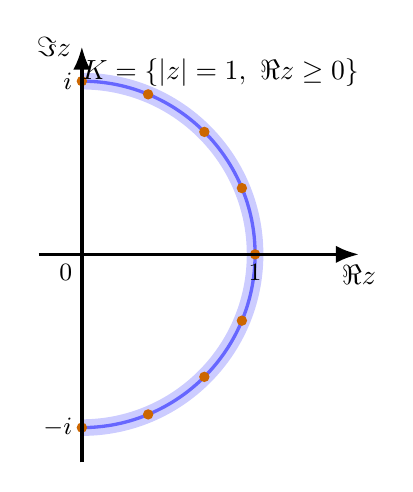
\begin{tikzpicture}[scale=2.2]
		% arc K and soft highlight
		\draw[blue!20,line width=6pt] (0,-1) arc (-90:90:1);
		\draw[very thick,blue!60] (0,-1) arc (-90:90:1);
		% nodes (here n=8 for illustration)
		\foreach \k in {0,...,8}{
			\pgfmathsetmacro{\t}{-90 + 180*\k/8}
			\fill[orange!80!black] ({cos(\t)},{sin(\t)}) circle (0.03);
		}
		% axes
		\draw[-Latex,very thick] (-0.25,0)--(1.6,0) node[below] {$\Re z$};
		\draw[-Latex,very thick] (0,-1.2)--(0,1.2) node[left] {$\Im z$};
		\node[below left] at (0,0) {\small $0$};
		\node[below] at (1,0) {\small $1$};
		\node[left] at (0,1) {\small $i$};
		\node[left] at (0,-1) {\small $-i$};
		\node at (0.8,1.05) {$K=\{|z|=1,\ \Re z\ge 0\}$};
	\end{tikzpicture}
	\caption{Right semicircle $K$ and equally spaced interpolation nodes $z_k=e^{it_k}$.}
\end{figure}

% ---------- Optional: error of p_2 along the arc ----------
\begin{figure}[H]
	\centering
	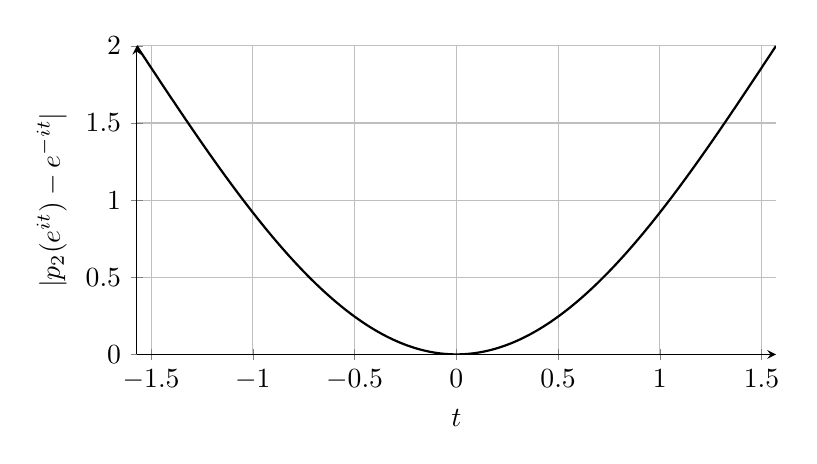
\begin{tikzpicture}
		\begin{axis}[
			width=.8\linewidth, height=5.5cm,
			domain=-pi/2:pi/2, samples=400,
			axis lines=left, xlabel={$t$}, ylabel={$|p_2(e^{it})-e^{-it}|$},
			grid=both, ymin=0
			]
			% p2(z)=z^2 - z + 1, z=e^{it}; error magnitude vs t
			\addplot[thick]
			{ sqrt( (cos(2*x)+1-2*cos(deg(x)))^2 + (sin(2*x))^2 ) };
		\end{axis}
	\end{tikzpicture}
	\caption{Pointwise error of $p_2(z)=z^2-z+1$ along $z=e^{it}$, $t\in[-\pi/2,\pi/2]$.}
\end{figure}

% ===================== END CONTENT =====================
\begin{exercise}{Polynomial characterization of holomorphicity on Runge domains}{poly-char}
	Let $U\subset\mathbb C$ be bounded, open, and suppose $\mathbb C\setminus U$ is connected.
	Show that $f:U\to\mathbb C$ is holomorphic iff for every compact $K\Subset U$ and every
	$\varepsilon>0$ there exists a polynomial $P$ with
	\[
	\sup_{z\in K}|f(z)-P(z)|<\varepsilon.
	\]
\end{exercise}

\begin{definition}
	\textbf{Polynomial hull in the plane.} For a compact $K\subset\mathbb C$, let
	\[
	\widehat K:=K\cup\!\!\!\bigcup_{\ \ \Omega\text{ bounded component of }\mathbb C\setminus K}\!\!\!\!\overline{\Omega}.
	\]
	Then $\mathbb C\setminus\widehat K$ is connected. If $K\Subset U$ and $\mathbb C\setminus U$ is connected,
	then $\widehat K\Subset U$.
\end{definition}

\begin{theorem}[Mergelyan]
	If $K\subset\mathbb C$ is compact with connected complement, and $g$ is continuous on $K$
	and holomorphic on $\operatorname{int}K$, then for every $\varepsilon>0$ there exists a polynomial
	$P$ with $\sup_{K}|g-P|<\varepsilon$.
\end{theorem}

\begin{proof}[Solution]
	($\Rightarrow$) Assume $f$ holomorphic on $U$, let $K\Subset U$, and set $\widehat K$ as above.
	Then $\widehat K\Subset U$ and $\mathbb C\setminus\widehat K$ is connected, hence by Mergelyan
	there is a polynomial $P$ with $\sup_{\widehat K}|f-P|<\varepsilon$, thus in particular on $K$.
	
	($\Leftarrow$) Assume: for every $K\Subset U$ and $\varepsilon>0$ there is a polynomial
	$P$ with $\sup_K|f-P|<\varepsilon$. Let $K_1\Subset K_2\Subset\cdots\Subset U$ with
	$\bigcup_m K_m=U$ and choose polynomials $P_m$ with $\sup_{K_m}|f-P_m|<1/m$.
	Then $P_m\to f$ uniformly on each $K_\ell$, so by Weierstrass’ theorem the limit $f$
	is holomorphic on $U$.
\end{proof}

\begin{remark}
	On $U=\{\,|z|<1\,\}$ one may take $P_n$ to be partial sums of the Taylor series of $f$ at $0$,
	which converge uniformly on $K=\{\,|z|\le r\,\}$ for each $r<1$. The theorem shows such
	polynomial approximation on every compact holds on any bounded $U$ with connected complement.
\end{remark}
% ======= Notation: compact inclusion =======
\begin{definition}
	\textbf{Compact inclusion.}
	For sets $K\subset U\subset\mathbb C$, we write $K\Subset U$ if $K\subset U$ and
	$\overline K$ is compact with $\overline K\subset U$. Equivalently, in the plane
	$\operatorname{dist}(K,\partial U)>0$.
\end{definition}

\begin{figure}[H]
	\centering
	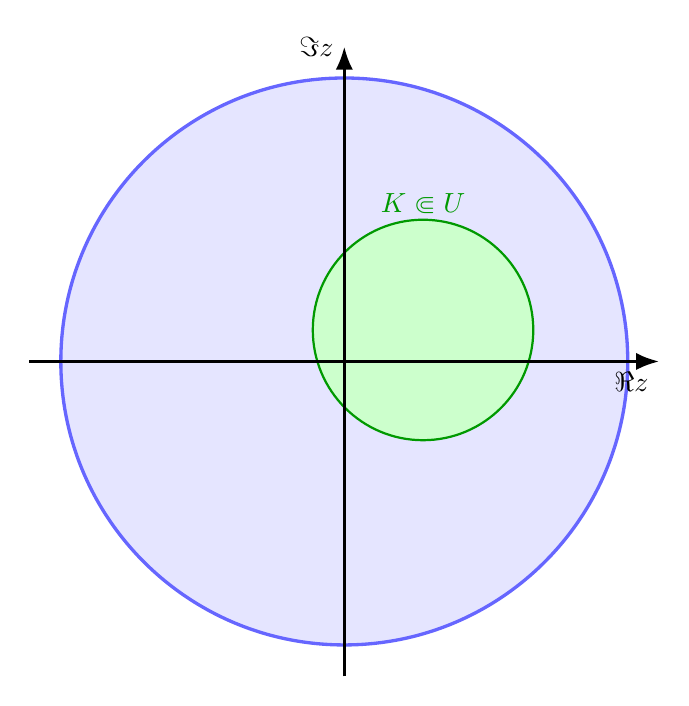
\begin{tikzpicture}[scale=2.0]
		% U (open region)
		\fill[blue!10] (0,0) circle (1.8);
		\draw[blue!60,very thick] (0,0) circle (1.8) node[above right] {$U$};
		% K compactly contained
		\fill[green!20,draw=green!60!black,thick] (0.5,0.2) circle (0.7);
		\node[green!60!black] at (0.5,1.0) {$K\Subset U$};
		% axes on top
		\draw[-Latex,very thick] (-2.0,0)--(2.0,0) node[below left] {$\Re z$};
		\draw[-Latex,very thick] (0,-2.0)--(0,2.0) node[left] {$\Im z$};
	\end{tikzpicture}
	\caption{$K\Subset U$: $K$ sits a positive distance away from $\partial U$.}
\end{figure}

% ======= Convergence notions =======
\begin{definition}
	\textbf{Pointwise and uniform convergence.} Let $E$ be a set and $(f_n)$ functions on $E$.
	\begin{itemize}
		\item $f_n\to f$ pointwise on $E$ if $\forall x\in E,\ \forall\varepsilon>0$,
		$\exists N=N(\varepsilon,x)$ with $|f_n(x)-f(x)|<\varepsilon$ for $n\ge N$.
		\item $f_n\to f$ uniformly on $E$ if
		$\displaystyle \sup_{x\in E}|f_n(x)-f(x)|\xrightarrow[n\to\infty]{}0.$
		\item $f_n\to f$ \emph{locally uniformly} on an open $U$ if for every $K\Subset U$,
		the convergence is uniform on $K$.
	\end{itemize}
\end{definition}

\begin{remark}
	On a compact set $K$, uniform on $K$ $\iff$ convergence in the sup norm $\|\cdot\|_\infty$.
	If $U$ is open, ``locally uniform'' means uniform on every $K\Subset U$; on a compact $U$
	this reduces to uniform on $U$.
\end{remark}

% ======= Examples =======
\begin{example}[Uniform vs nonuniform convergence]
	\hfill
	\begin{enumerate}
		\item Uniform: $f_n(x)=\dfrac{x}{n+x}$ on $[0,1]$; then
		$\sup_{[0,1]}|f_n|=\frac{1}{n+1}\to0$, so $f_n\to0$ uniformly.
		\item Nonuniform: $f_n(x)=x^n$ on $[0,1]$; then $f_n\to f$ pointwise with
		$f=\mathbf 1_{\{1\}}$, but not uniformly, since
		$\sup_{x\in[0,1)}|x^n-0|=1$ for all $n$.
	\end{enumerate}
\end{example}

\begin{figure}[H]
	\centering
	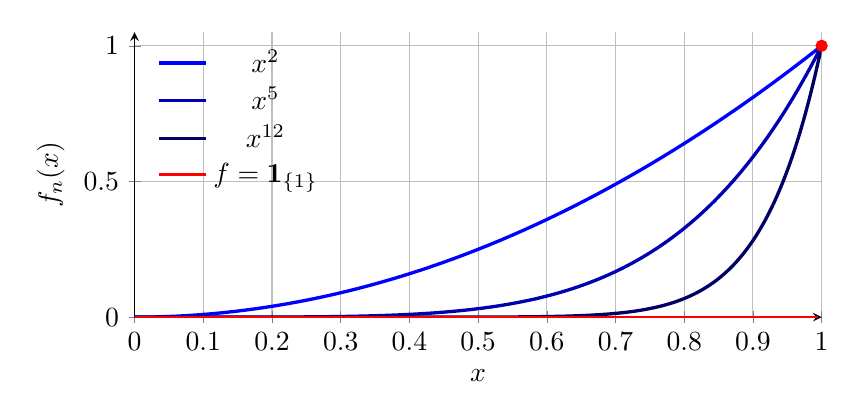
\begin{tikzpicture}
		\begin{axis}[
			width=.85\linewidth, height=5.2cm,
			xmin=0, xmax=1, ymin=0, ymax=1.05,
			axis lines=left, xlabel={$x$}, ylabel={$f_n(x)$},
			legend style={at={(0.02,0.98)},anchor=north west,draw=none,fill=none},
			grid=both
			]
			\addplot[blue,very thick,domain=0:1,samples=400]{x^(2)}; \addlegendentry{$x^2$}
			\addplot[blue!70!black,very thick,domain=0:1,samples=400]{x^(5)}; \addlegendentry{$x^5$}
			\addplot[blue!40!black,very thick,domain=0:1,samples=400]{x^(12)}; \addlegendentry{$x^{12}$}
			\addplot[red,thick,domain=0:0.995,samples=2]{0};
			\addplot[only marks,mark=*,red] coordinates {(1,1)}; \addlegendentry{$f=\mathbf 1_{\{1\}}$}
		\end{axis}
	\end{tikzpicture}
	\caption{$x^n\to \mathbf 1_{\{1\}}$ pointwise on $[0,1]$, but not uniformly.}
\end{figure}

\begin{example}[Uniform vs nonuniform approximation by series]
	Let $S_n(x)=\sum_{k=0}^{n}x^k$.
	\begin{itemize}
		\item On $[0,b]$ with $0<b<1$: $\left\|\dfrac{1}{1-x}-S_n\right\|_{[0,b]}
		=\sup_{[0,b]}\frac{x^{n+1}}{1-x}\le \frac{b^{n+1}}{1-b}\to0$ (uniform).
		\item On $[0,1)$: not uniform, since $\sup_{x\in[0,1)}\dfrac{x^{n+1}}{1-x}=+\infty$.
	\end{itemize}
\end{example}
\begin{exercise}{Polynomials $p_n$ with $p_n(0)=1$ and $p_n(z)\to0$ for $z\neq0$}{poly-vanish-off-zero}
	Does there exist a sequence of complex polynomials $(p_n)$ such that
	$p_n(0)=1$ for all $n$ and $p_n(z)\to 0$ for each $z\in\mathbb C\setminus\{0\}$?
\end{exercise}

\begin{definition}
	For $n\in\mathbb N$ let
	\[
	K_n:=\Bigl\{\,z:\ \tfrac1n\le |z|\le n,\ \ |\arg z|\le \pi-\tfrac1n\,\Bigr\}
	\quad(\text{a ``slit annulus''}).
	\]
	Then $K_n$ is compact, $K_n\Subset\mathbb C\setminus\{0\}$, and
	$\bigcup_{n\ge1}K_n=\mathbb C\setminus\{0\}$. The complement
	$\mathbb C\setminus K_n$ is \emph{connected} because the missing
	thin sector joins the inner and outer parts.
\end{definition}

\begin{theorem}
	There exists a sequence of polynomials $(p_n)$ with $p_n(0)=1$ for all $n$ and
	$p_n(z)\to0$ for every $z\neq0$.
\end{theorem}

\begin{proof}
	Fix $n$. Define a function on the compact set $E_n:=K_n\cup\{0\}$ by
	\[
	\phi_n(z)=\begin{cases}
		0,&z\in K_n,\\
		1,&z=0.
	\end{cases}
	\]
	This $\phi_n$ is continuous on $E_n$ and holomorphic on $\operatorname{int}E_n$
	(the interior is the slit annulus, where $\phi_n\equiv0$). Since
	$\mathbb C\setminus E_n=(\mathbb C\setminus K_n)\setminus\{0\}$ is still connected,
	Mergelyan’s theorem applies: for each $\varepsilon_n>0$ there exists a polynomial
	$P_n$ with
	\[
	\sup_{z\in E_n}|P_n(z)-\phi_n(z)|<\varepsilon_n.
	\]
	Choose $\varepsilon_n\le \tfrac{1}{4}$ so that in particular $|P_n(0)-1|<\tfrac14$.
	Set
	\[
	p_n(z):=\frac{P_n(z)}{P_n(0)}.
	\]
	Then $p_n$ is a polynomial with $p_n(0)=1$, and for $z\in K_n$,
	\[
	|p_n(z)|=\frac{|P_n(z)|}{|P_n(0)|}\le
	\frac{|P_n(z)-\phi_n(z)|}{|P_n(0)|}\le \frac{\varepsilon_n}{1-\varepsilon_n}
	\le 2\varepsilon_n .
	\]
	Now fix $z\neq0$. For $n$ large enough we have $z\in K_n$, hence
	$|p_n(z)|\le 2\varepsilon_n \to 0$ as $n\to\infty$. This proves the claim.
\end{proof}

\begin{remark}
	No uniformity on large discs is possible: if a polynomial $q$ were tiny on the
	circle $|z|=R$, the maximum modulus principle on $|z|\le R$ would force $|q(0)|$
	tiny as well. The slit ensures $\mathbb C\setminus K_n$ is connected, allowing
	Mergelyan, but $K_n$ does \emph{not} enclose $0$, so there is no contradiction
	with $p_n(0)=1$.
\end{remark}

% needs: \usepackage{tikz} \usetikzlibrary{arrows.meta}
\begin{figure}[H]
	\centering
	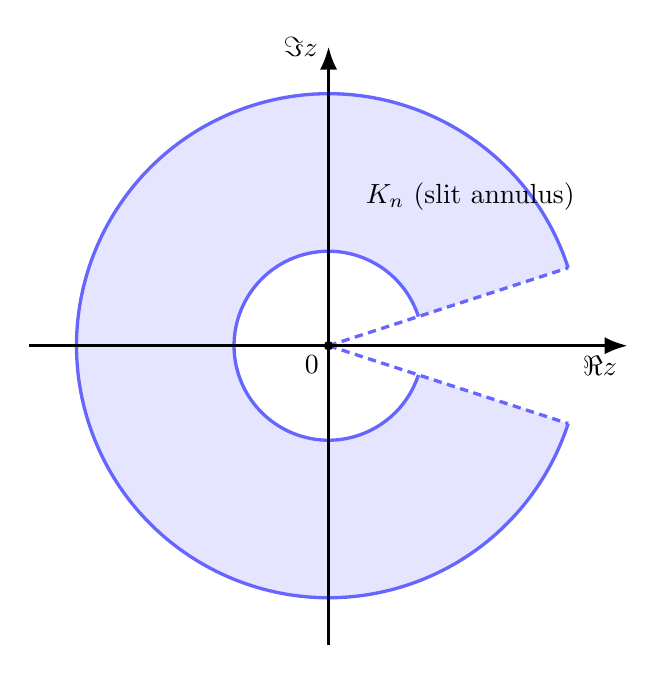
\begin{tikzpicture}[scale=2.0]
		% outer/inner radii
		\def\R{1.6}
		\def\r{0.6}
		\def\gap{18} % opening angle in degrees
		
		% fill the slit annulus K_n
		\fill[blue!10] (0,0) -- (\gap:\r) arc (\gap:360-\gap:\r)
		-- (360-\gap:\R) arc (360-\gap:\gap:\R) -- cycle;
		\draw[blue!60,very thick] (\gap:\r) arc (\gap:360-\gap:\r);
		\draw[blue!60,very thick] (\gap:\R) arc (\gap:360-\gap:\R);
		% the missing narrow sector (complement channel)
		\draw[blue!60,very thick,densely dashed] (0,0) -- (\gap:\R);
		\draw[blue!60,very thick,densely dashed] (0,0) -- (360-\gap:\R);
		
		% the point 0
		\fill (0,0) circle (0.03) node[below left] {$0$};
		
		% label
		\node at (0.9,0.95) {$K_n$ (slit annulus)};
		% axes
		\draw[-Latex,very thick] (-1.9,0)--(1.9,0) node[below left] {$\Re z$};
		\draw[-Latex,very thick] (0,-1.9)--(0,1.9) node[left] {$\Im z$};
	\end{tikzpicture}
	\caption{A typical $K_n$: annulus $\{1/n\le|z|\le n\}$ minus a thin sector; its complement is connected.}
\end{figure}

\begin{exercise}{Uniform polynomial approximation on an annulus forces extension} -{annulus-extension}
	Let $A=\{z\in\mathbb C: \tfrac12\le |z|\le 1\}$ and let $f:A\to\mathbb C$ be continuous on $A$ and
	holomorphic on $\operatorname{int}A$. Suppose polynomials $p_n$ converge uniformly to $f$ on $A$.
	Show there exists $g:\{|z|\le1\}\to\mathbb C$ continuous, holomorphic on $\{|z|<1\}$, with $g=f$ on $A$.
\end{exercise}

\begin{proof}
	Fix $\rho\in(\tfrac12,1)$. Since $|z|=\rho\subset A$ and $p_n\to f$ uniformly on $A$,
	the sequence $(p_n)$ is uniformly Cauchy on $|z|=\rho$:
	$\sup_{|z|=\rho}|p_n-p_m|\to0$ as $n,m\to\infty$.
	For each $n,m$ the difference $p_n-p_m$ is entire, hence by the maximum modulus principle on
	the closed disk $\overline D_\rho:=\{|z|\le\rho\}$,
	\[
	\sup_{|z|\le\rho}|p_n(z)-p_m(z)|\le \sup_{|z|=\rho}|p_n(z)-p_m(z)|\xrightarrow[n,m\to\infty]{}0.
	\]
	Thus $(p_n)$ converges uniformly on $\overline D_\rho$ to some function $g_\rho$ that is holomorphic on $|z|<\rho$.
	
	If $\rho'<\rho$ are both $>\tfrac12$, then $p_n\to g_{\rho'}$ on $\overline D_{\rho'}$ and $p_n\to g_\rho$ on
	$\overline D_\rho$, so $g_{\rho'}=g_\rho$ on $|z|<\rho'$. Define $g$ on $\{|z|<1\}=\bigcup_{\rho>1/2}\{|z|<\rho\}$ by
	$g:=g_\rho$ on $|z|<\rho$; this is well defined and holomorphic.
	
	On $A\cap\{|z|\le\rho\}=\{\tfrac12\le|z|\le\rho\}$ we have $p_n\to f$ (by hypothesis) and $p_n\to g$
	(by uniform convergence on $\overline D_\rho$), hence $g=f$ there. Letting $\rho\uparrow1$ yields $g=f$ on all of $A$.
	Finally, $g$ is continuous on $\{|z|\le1\}$ because it is holomorphic on $\{|z|<1\}$ and coincides with the continuous
	$f$ on $|z|=1$.
\end{proof}

\begin{remark}
	As a corollary, $1/z$ cannot be approximated uniformly by polynomials on $A$, since such an approximation would
	produce a holomorphic extension across $0$.
\end{remark}

% --- optional figure (annulus, circle |z|=rho, and the disk where MMP is used) ---
\begin{figure}[H]
	\centering
	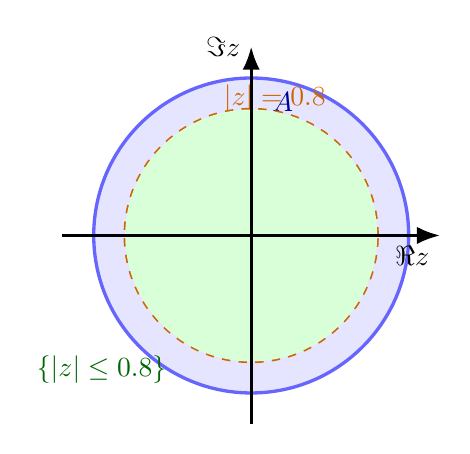
\begin{tikzpicture}[scale=2.0]
		% annulus A
		\fill[blue!10] (0,0) circle (1);
		\fill[white] (0,0) circle (0.5);
		\draw[blue!60,very thick] (0,0) circle (1);
		\draw[blue!60,very thick] (0,0) circle (0.5);
		\node[blue!60!black] at (0.2,0.85) {$A$};
		
		% circle |z|=rho
		\def\rho{0.8}
		\draw[orange!80!black,very thick,dashed] (0,0) circle (\rho);
		\node[orange!80!black] at (0.15,\rho+0.07) {$|z|=\rho$};
		
		% inner disk where we apply MMP to differences
		\fill[green!15] (0,0) circle (\rho);
		\node[green!40!black] at (-0.95,-0.85) {$\{|z|\le \rho\}$};
		
		% axes
		\draw[-Latex,very thick] (-1.2,0)--(1.2,0) node[below left] {$\Re z$};
		\draw[-Latex,very thick] (0,-1.2)--(0,1.2) node[left] {$\Im z$};
	\end{tikzpicture}
	\caption{Fix $\rho\in(\tfrac12,1)$. Uniform convergence on $|z|=\rho$ and MMP make $(p_n)$ Cauchy on $\{|z|\le\rho\}$,
		giving a holomorphic limit inside; letting $\rho\uparrow1$ fills the disk and matches $f$ on $A$.}
\end{figure}

\begin{figure}[H]
	\centering
	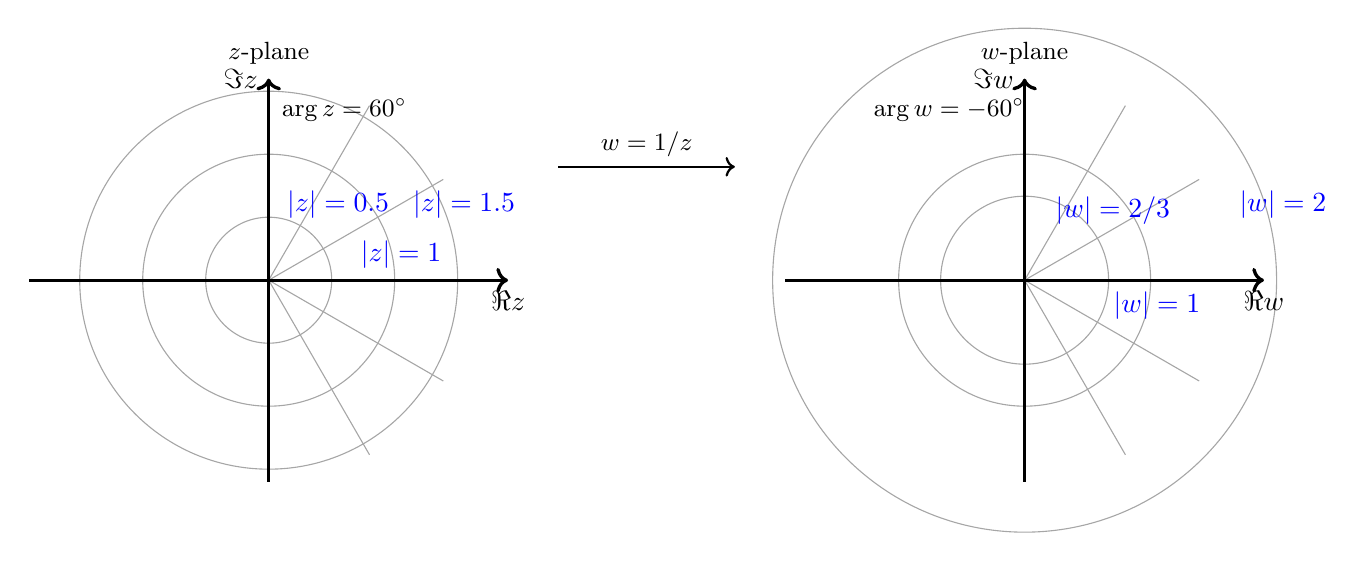
\begin{tikzpicture}[scale=1.6]
		% LEFT: preimage (z-plane)
		\begin{scope}
			\node at (0,1.8) {\small $z$-plane};
			% rays
			\foreach \ang in {-60,-30,0,30,60}{
				\draw[gray!70] (0,0) -- ({1.6*cos(\ang)},{1.6*sin(\ang)});
			}
			% circles
			\foreach \r in {0.5,1,1.5}{
				\draw[gray!70] (0,0) circle (\r);
			}
			\draw[->,very thick] (-1.9,0)--(1.9,0) node[below] {$\Re z$};
			\draw[->,very thick] (0,-1.6)--(0,1.6) node[left] {$\Im z$};
			\node[blue] at (1.05,0.2) {$|z|=1$};
			\node[blue] at (1.55,0.6) {$|z|=1.5$};
			\node[blue] at (0.55,0.6) {$|z|=0.5$};
			\node at (0.6,1.35) {\small $\arg z=60^\circ$};
		\end{scope}
		
		% RIGHT: image (w-plane)
		\begin{scope}[xshift=6cm]
			\node at (0,1.8) {\small $w$-plane};
			% images: rays reflect, radii invert
			\foreach \ang in {-60,-30,0,30,60}{
				\draw[gray!70] (0,0) -- ({1.6*cos(-\ang)},{1.6*sin(-\ang)});
			}
			\foreach \R in {2/3,1,2}{
				\draw[gray!70] (0,0) circle (\R);
			}
			\draw[->,very thick] (-1.9,0)--(1.9,0) node[below] {$\Re w$};
			\draw[->,very thick] (0,-1.6)--(0,1.6) node[left] {$\Im w$};
			\node[blue] at (1.05,-0.2) {$|w|=1$};
			\node[blue] at (2.05,0.6) {$|w|=2$};
			\node[blue] at (0.7,0.55) {$|w|=2/3$};
			\node at (-0.6,1.35) {\small $\arg w=-60^\circ$};
		\end{scope}
		
		% arrow
		\draw[->,thick] (2.3,0.9) -- (3.7,0.9) node[midway,above] {\small $w=1/z$};
	\end{tikzpicture}
	\caption{Circles centered at $0$ invert radii, rays flip angles. The unit circle is fixed (parameters reverse).}
\end{figure}



\begin{figure}[H]
	\centering
	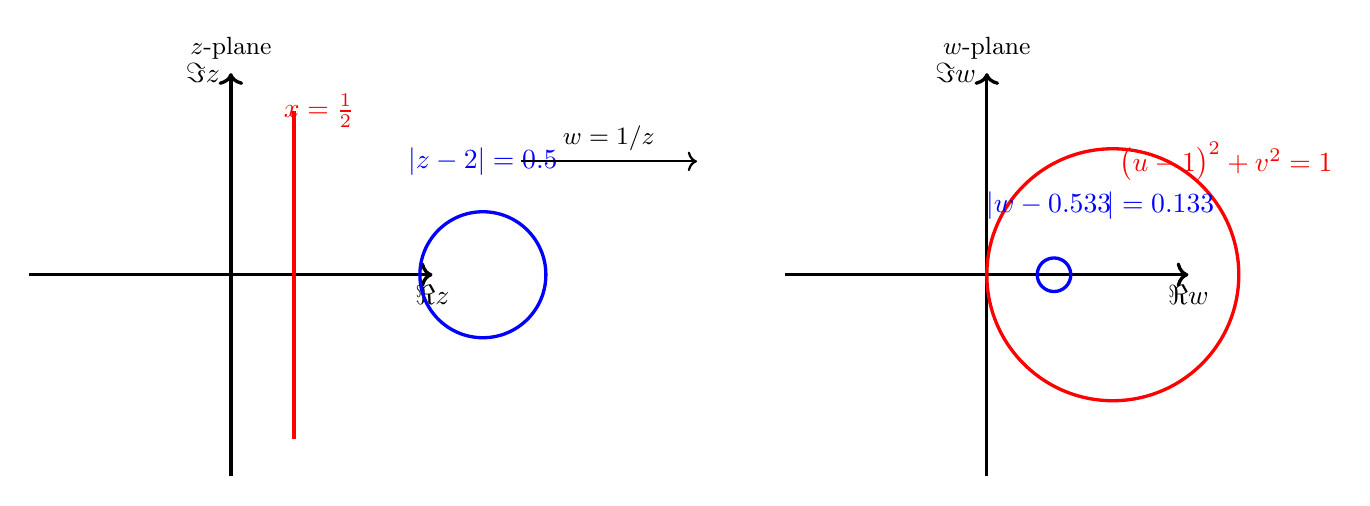
\begin{tikzpicture}[scale=1.6]
		% LEFT: line x=1/2 in z-plane
		\begin{scope}
			\node at (0,1.8) {\small $z$-plane};
			\draw[->,very thick] (-1.6,0)--(1.6,0) node[below] {$\Re z$};
			\draw[->,very thick] (0,-1.6)--(0,1.6) node[left] {$\Im z$};
			\draw[red,very thick] (0.5,-1.3) -- (0.5,1.3);
			\node[red] at (0.7,1.3) {$x=\tfrac12$};
			% a circle not through 0: |z-2|=0.5
			\draw[blue,very thick] (2,0) circle (0.5);
			\node[blue] at (2,0.9) {$|z-2|=0.5$};
		\end{scope}
		
		% RIGHT: images in w-plane
		\begin{scope}[xshift=6cm]
			\node at (0,1.8) {\small $w$-plane};
			\draw[->,very thick] (-1.6,0)--(1.6,0) node[below] {$\Re w$};
			\draw[->,very thick] (0,-1.6)--(0,1.6) node[left] {$\Im w$};
			% image of x=1/2 is circle centered at (1,0) radius 1
			\draw[red,very thick] (1,0) circle (1);
			\node[red] at (1.9,0.9) {$\big(u-1\big)^2+v^2=1$};
			% image of |z-2|=0.5: center = a/(|a|^2-R^2)=2/(4-0.25)=0.533..., radius=R/(|a|^2-R^2)=0.5/3.75
			\draw[blue,very thick] (0.5333,0) circle (0.1333);
			\node[blue] at (0.9,0.55) {$|w-0.533\!|=0.133$};
		\end{scope}
		
		\draw[->,thick] (2.3,0.9) -- (3.7,0.9) node[midway,above] {\small $w=1/z$};
	\end{tikzpicture}
	\caption{Under $w=1/z$: lines not through $0$ become circles through $0$; circles not through $0$ remain circles with transformed center/radius.}
\end{figure}

\begin{exercise}{Irrationality and algebraicity}{irr-alg}
	\begin{enumerate}
		\item \textbf{Irrational sums/powers.}
		\begin{enumerate}
			\item $(\sqrt3+\sqrt5)\notin\mathbb Q$. If $\sqrt3+\sqrt5=r\in\mathbb Q$, then
			$r^2=8+2\sqrt{15}$, hence $\sqrt{15}=(r^2-8)/2\in\mathbb Q$, impossible.
			\item $e^2\notin\mathbb Q$. Suppose $e^2=a/b\in\mathbb Q$. For $N\ge\max\{2,b\}$,
			both $N!e^2$ and $N!\sum_{n=0}^{N}\frac{2^n}{n!}$ are integers, but
			\[
			0<N!\Bigl(e^2-\sum_{n=0}^{N}\frac{2^n}{n!}\Bigr)
			=\sum_{n=N+1}^{\infty}\frac{2^n N!}{n!}
			<\sum_{k=1}^{\infty}\Bigl(\frac{2}{N+1}\Bigr)^k<1,
			\]
			a contradiction.
		\end{enumerate}
		
		\item \textbf{Algebraic numbers and coefficients.}
		\begin{enumerate}
			\item A real $\alpha$ is algebraic iff it is a zero of some nonzero polynomial
			with rational coefficients. ($\Leftarrow$) Clear after clearing denominators.
			($\Rightarrow$) Integers are rationals.
			\item \emph{False} that rational coefficients are forced. Example:
			$(x-\sqrt2)(x-\sqrt3)=x^2-(\sqrt2+\sqrt3)x+\sqrt6$. The roots are algebraic,
			but the coefficients are not rational.
		\end{enumerate}
	\end{enumerate}
\end{exercise}


	
\end{document}

